\documentclass[a4paper,11pt]{report}
\usepackage{fullpage}

\usepackage{"../../info/packages"}
\usepackage{"../../info/nomenclature"}

\usepackage{scalerel}
\usepackage{subfiles}

\newcommand{\xvecdot}{\dot{\xvec}}
\newcommand{\xdot}{\dot{x}}
\newcommand{\qvecdot}{\dot{\qvec}}
\newcommand{\qdot}{\dot{q}}

\setlength{\cellspacetoplimit}{3pt}
\setlength{\cellspacebottomlimit}{3pt}

\title{Introduction}
\author{Alejandro Campos}

\begin{document}
\maketitle
\tableofcontents

%########################################################################
\chapter{Governing equations}
%########################################################################

%------------------------------------------------------------------------
\section{Particle description}
%------------------------------------------------------------------------
\begin{table}[H]
    \renewcommand{\arraystretch}{1.5}
    \centering
    \caption{Various coordinates of classical mechanics. }
    \label{tb:classical_mechanics_coordinates}
     \begin{tabular}{|l|l|l|}
        \hline
        Classical coordinates & $\xvec(t)$ & $\vvec(t)$ \\
        \hline
        Generalized coordinates  & $\qvec$ & $\qvecdot$ \\
        \hline
        Canonical coordinates & $\qvec$ & $\pvec$ \\
        \hline
        Time-dependent canonical coordinates & $\tilde{\qvec}(t)$ & $ \tilde{\pvec}(t)$ \\
        \hline
     \end{tabular}
\end{table}
    
%--------------------------------------------
\subsection{Lagrangian mechanics}
%--------------------------------------------
    
\begin{itemize}
    \item Define the position $\xvec = \xvec(t)$ and velocity $\vvec = \vvec(t)$ of a particle. 
    
    \item Define the Lagrangian as $L = L(\qvec, \qvecdot,t)$, where $\qvec$ and $\qvecdot$ are the generalized position and generalized velocity, respectively. 
    
    \item The equations of motion are obtained from the Euler-Lagrange equation, which is 
    \begin{equation}
    \frac{d}{dt} \left [ \left ( \frac{\partial L}{\partial \qdot_i } \right )_{\qvec =  \xvec, \qvecdot = \vvec }  \right] = \left ( \frac{\partial L}{\partial q_i} \right )_{ \qvec =  \xvec, \qvecdot = \vvec} .
    \end{equation}
    
    \item For example, the Lagrangian of a particle in an electromagnetic field where $\phi = \phi(\qvec,t)$ is the electric potential and $\Avec = \Avec(\qvec,t)$ is the magnetic potential, is
    \begin{equation}
    L = \frac{1}{2} m \qdot_i \qdot_i + e \qdot_i A_i - e\phi.
    \end{equation}
    The derivatives in the Euler-Lagrange equation are
    \begin{equation}
    \frac{\partial L}{\partial q_i} = e \qdot_j \frac{\partial A_j }{\partial q_i} - e \frac{\partial \phi}{ \partial q_i}
    \end{equation}
    \begin{equation}
    \frac{\partial L}{\partial \qdot_i} = m \qdot_i + e A_i 
    \end{equation}
    \begin{align}
    \frac{d}{dt}\left [ \left ( \frac{\partial L}{\partial \qdot_i } \right )_{\qvec =  \xvec, \qvecdot= \vvec }  \right] &= \frac{d}{dt} \left [ m v_i + e A_i(\xvec,t) \right ] \nonumber \\
    &= m \frac{ d v_i}{dt} + e v_j \left (\frac{\partial A_i}{\partial q_j} \right )_{\qvec = \xvec} +  e \left (\frac{\partial A_i}{\partial t} \right )_{\qvec = \xvec} .
    \end{align}
    Thus, the Euler-Lagrange equation becomes
    \begin{equation}
    \label{eq:lag_mech_tensor_lorentz}
    m \frac{ d v_i}{dt} = \left ( - e v_j \frac{\partial A_i}{\partial q_j} - e\frac{\partial A_i}{\partial t} + e v_j \frac{\partial A_j }{\partial q_i} - e \frac{\partial \phi}{ \partial q_i}\right )_{\qvec = \xvec}.
    \end{equation}
    In vector notation, this is written as
    \begin{equation}
        m \frac{d \vvec}{dt} = \left(-e\vvec \cdot \nabla_q \Avec - e \frac{\partial \Avec}{\partial t} + e \nabla_q (\vvec \cdot \Avec) - e \nabla_q \phi \right)_{\qvec = \xvec}.
    \end{equation}
    Using the vector identity (4) from Griffiths book, the above can be expressed as
    \begin{equation}
    m \frac{d\vvec}{dt} = e \left ( \Evec + \vvec \times \Bvec \right)_{\qvec = \xvec},
    \end{equation}
    where $\Evec = \Evec(\qvec,t)$ and $\Bvec = \Bvec(\qvec,t)$.
\end{itemize}
    
%--------------------------------------------
\subsection{Hamiltonian mechanics}
%--------------------------------------------
\begin{itemize}
    \item Define the Hamiltonian as $H = H(\qvec, \pvec, t)$, where $\qvec$ and $\pvec$ are the canonical position and momentum. For all purposes here, the canonical position is the same as the generalized position.
    
    \item The Hamiltonian is obtained from the Lagrangian using
    \begin{equation}
    H = \left ( \qvecdot \cdot \pvec - L \right)_{\qvecdot = \fvec(\qvec, \pvec)},
    \end{equation} 
    where the dependency of $\qvecdot$ on $\qvec$ and $\pvec$ is obtained from evaluating
    \begin{equation}
    \label{eq:v_from_qp}
    \pvec = \frac{ \partial L}{\partial \qvecdot}.
    \end{equation}
    
    \item For example, for a particle in an electromagnetic field we have
    \begin{equation}
    H = \left [ \qdot_i p_i - \left ( \frac{1}{2} m \qdot_i \qdot_i + e \qdot_i A_i - e\phi \right ) \right]_{\qvecdot = f(\qvec, \pvec)}. 
    \end{equation}
    Evaluating \cref{eq:v_from_qp} gives $ p_i = m \qdot_i + e A_i $, which allows us to express $\qvecdot$ in terms of $\qvec$ and $\pvec$ as $\qdot_i = \frac{1}{m} (p_i - eA_i )$. Thus
    \begin{align}
    H &= \frac{1}{m} (p_i - eA_i)p_i - \frac{1}{2m} (p_i - eA_i) (p_i-eA_i) - e\frac{1}{m} (p_i -eA_i) A_i + e\phi \nonumber \\
    & = \frac{1}{2m} (p_i -eA_i) (p_i -eA_i) + e\phi.
    \end{align}
    
    \item We introduce the variables $\tilde{\qvec} = \tilde{\qvec}(t)$ and $\tilde{\pvec} = \tilde{\pvec}(t)$, which are defined by
    \begin{align}
    \tilde{\qvec} &= \xvec \\ 
    \tilde{\pvec} & = \left ( \frac{\partial L}{\partial \qvecdot} \right)_{\qvec = \xvec, \qvecdot = \vvec}
    \end{align}
    
    \item The equations of motion are obtained from
    \begin{align}
    \frac{d \tilde{q}_i}{dt} &= \left ( \frac{ \partial H}{\partial p_i} \right )_{\qvec = \tilde{\qvec}, \pvec = \tilde{\pvec}} \\
    \frac{d \tilde{p}_i}{dt} & = -\left ( \frac{ \partial H}{\partial q_i} \right )_{\qvec = \tilde{\qvec}, \pvec = \tilde{\pvec}} \label{eq:hamil_p}
    \end{align}
    
    \item For example, for a particle in an electromagnetic field we have
    \begin{equation}
    \tilde{p}_i = mv_i + e A_i(\xvec,t)
    \end{equation}
    and thus
    \begin{align}
    \frac{d \tilde{p}_i}{dt} & = m \frac{d v_i}{dt} + e v_j \left ( \frac{\partial A_i}{\partial q_j} \right)_{\qvec = \xvec} + e \left ( \frac{ \partial A_i}{\partial t} \right)_{\qvec = \xvec}.
    \end{align}
    \begin{align}
    \frac{\partial H}{\partial q_i} &= \frac{\partial}{\partial q_i} \left [ \frac{1}{2m} (p_j -eA_j) (p_j -eA_j) + e\phi \right] \nonumber \\
    & = \frac{1}{m} (p_j -eA_j) \frac{\partial}{\partial q_i} (p_j - eA_j) + e\frac{\partial \phi}{\partial q_i} \nonumber \\
    &  = -\frac{e}{m} (p_j - eA_j) \frac{\partial A_j}{\partial q_i} + e \frac{\partial \phi}{\partial q_i}
    \end{align}
    \begin{align}
    \left ( \frac{ \partial H}{\partial q_i} \right )_{\qvec = \tilde{\qvec}, \pvec = \tilde{\pvec}} &= -\frac{e}{m} \left [ m v_j + eA_j(\xvec,t) - eA_j(\xvec,t) \right ] \left ( \frac{\partial A_j}{\partial q_i} \right)_{\qvec = \xvec} + e \left ( \frac{\partial \phi}{\partial q_i} \right)_{\qvec = \xvec} \nonumber \\
    & = \left( -e v_j \frac{\partial A_j}{\partial q_i} + e \frac{ \partial \phi}{\partial q_i} \right)_{\qvec = \xvec} .
    \end{align}
    
    \Cref{eq:hamil_p} thus leads to
    \begin{equation}
    m \frac{d v_i}{dt} = \left ( -e v_j \frac{ \partial A_i}{\partial q_j} - e \frac{ \partial A_i}{\partial t} + e v_j \frac{ \partial A_j}{\partial q_i} - e \frac{ \partial \phi}{\partial q_i} \right)_{\qvec = \xvec}.
    \end{equation}
    This is the same as \cref{eq:lag_mech_tensor_lorentz} and thus, as shown before, the above can be expressed as
    \begin{equation}
    \label{eq:single_particle_classical_mechanics}
    m \frac{d \vvec}{dt} = e \left ( \Evec + \vvec \times \Bvec \right)_{\qvec = \xvec}.
    \end{equation}
    
\end{itemize}

%------------------------------------------------------------------------
\section{Kinetic description}
%------------------------------------------------------------------------
We denote the distribution function for a species $s$ as $f_s = f_s(\rvec, \vvec, t)$, where $\rvec$ and $\vvec$ are the sample space variables for position and velocity. Note that the distribution function is appropriately normalized such that
\begin{equation}
\int f_s \, d\rvec d\vvec = N_s,
\end{equation}
where $N_s$ is the total number of particles corresponding to species $s$. 

The dynamics of a plasma can be characterized by the Boltzmann evolution equation for the distribution function of $N$ species along with Maxwell's equations
\begin{equation}
\label{eq:kinetic_equation}
\frac{\partial f_s}{\partial t} + \vvec \cdot \nabla f_s + \frac{Z_s e}{m_s} ( \Evec + \vvec \times \Bvec ) \cdot \nabla_v f_s = C_s + S_s
\end{equation}
\begin{equation}
\label{eq:maxwell_3}
\nabla \cdot \Evec = \frac{\rho_q}{\epsilon_0} 
\end{equation}
\begin{equation}
\label{eq:maxwell_4}
\nabla \cdot \Bvec = 0
\end{equation}
\begin{equation}
\label{eq:maxwell_1}
\nabla \times \Evec = -\frac{ \partial \Bvec}{\partial t}
\end{equation}
\begin{equation}
\label{eq:maxwell_2}
\nabla \times \Bvec = \mu_0 \Jvec + \mu_0 \epsilon_0 \frac{\partial \Evec}{\partial t}
\end{equation}
\begin{equation}
\Jvec = \sum_s^N Z_s e \int \vvec f_s \, d\vvec
\end{equation}
\begin{equation}
\rho_q = \sum_s^N Z_s e \int f_s \, d\vvec.
\end{equation}
In the above, 
\begin{itemize}
\item $m_s$ is the species mass
\item $e$ is the charge
\item $Z_s$ the charge number
\item $\Jvec = \Jvec(\rvec,t)$ the charge current
\item $\rho_q = \rho_q(\rvec,t)$ the charge density
\item $\Evec = \Evec(\rvec,t)$ the electric field
\item $\Bvec = \Bvec(\rvec,t)$ the magnetic field.
\end{itemize}
The terms $C_s$ and $S_s$ represent collision and source terms.

If we express the collision term in the usual way, that is $C_s = \sum_r^N C_{s r}$, then we can make the following statements:
\begin{enumerate}
\item Conservation of particles:
\begin{equation}
    \label{eq:coll_cons_particles}
    \int C_{ss} \, d\vvec = 0 \quad \forall s \qquad \qquad
    \int C_{sr} \,d\vvec = 0 \quad \forall s, r | r \ne s.
\end{equation}

\item Conservation of momentum:
\begin{equation}
    \label{eq:coll_cons_momentum}
    \int m_s \vvec C_{ss} \, d\vvec = 0 \quad \forall s \qquad \qquad \sum_s^N \sum_{r, r \ne s}^N \int m_s \vvec C_{sr} d\vvec = 0.
\end{equation}

\item Conservation of energy:
\begin{equation}
    \label{eq:coll_cons_energy}
    \int \frac{1}{2} m_s v^2 C_{ss} \, d\vvec = 0 \quad \forall s \qquad \qquad \sum_s^N \sum_{r, r \ne s}^N \int \frac{1}{2} m_s v^2 C_{sr} \, d\vvec = 0.
\end{equation}

\end{enumerate}

%------------------------------------------------------------------------
\section{Fluid description}
%------------------------------------------------------------------------
We now define the particle density $n_s = n_s(\rvec,t)$, the fluid velocity $\uvec_s = \uvec_s(\rvec,t)$ and the fluid energy per unit mass $E_s = E_s(\rvec,t)$ as follows
\begin{align}
n_s &= \int f_s \, d\vvec \\
\uvec_s &= \frac{1}{n_s} \int \vvec f_s \, d\vvec \\
E_s &= \frac{1}{n_s} \int \frac{1}{2} v^2 f_s \, d\vvec.
\end{align}
Their evolution equations are obtained by taking the appropriate moments of the Boltzmann plasma equation. Before doing so, we re-write the Boltzmann equation as
\begin{equation}
\label{eq:boltz_mod}
\frac{\partial f_s}{\partial t} + \nabla \cdot (\vvec f_s) + \nabla_v \cdot \left [ \frac{Z_s e}{m_s} ( \Evec + \vvec \times \Bvec ) f_s \right ] = C_s + S_s
\end{equation}

%--------------------------------------------
\subsection{Mass}
%--------------------------------------------
Integrating \cref{eq:boltz_mod} over all $\vvec$ we obtain
%\begin{empheq}[box=\widefbox]{equation}
\begin{equation}
\frac{\partial n_s}{\partial t} + \nabla \cdot \left ( n_s \uvec_s \right ) = \hat{S}_s
\end{equation}
%\end{empheq}
where 
\begin{equation}
\hat{S}_s = \int S_s \, d\vvec
\end{equation}
is an external source of mass.

%--------------------------------------------
\subsection{Momentum}
%--------------------------------------------
Multiplying \cref{eq:boltz_mod} by $\vvec$ and then integrating over all $\vvec$ leads to
\begin{multline}
\label{eq:mom_derv_1}
\frac{\partial n_s \uvec_s}{\partial t} + \nabla \cdot \left ( \int \vvec \vvec f_s \, d\vvec \right) + \int \nabla_v \cdot \left [ \vvec \frac{Z_s e}{m_s} ( \Evec + \vvec \times \Bvec ) f_s \right ] - \nabla_v \vvec \cdot \left [ \frac{Z_s e}{m_s} ( \Evec + \vvec \times \Bvec ) f_s \right ] \, d\vvec =\\
\sum_{r, r \ne s}^N \int \vvec C_{s r} \, d\vvec + \int \vvec S_s \, d\vvec.
\end{multline}
We note that the third term in \cref{eq:mom_derv_1} is zero since we are integrating over all space, and that $\nabla_v \vvec$ is the identity matrix. We thus have
\begin{multline}
\label{eq:mom_derv_2}
\frac{\partial n_s \uvec_s}{\partial t} + \nabla \cdot \left ( \int \vvec \vvec f_s \, d\vvec \right) - \frac{Z_s e n_s}{m_s} ( \Evec + \uvec_s \times \Bvec ) =\\
\sum_{r, r \ne s}^N \int \vvec C_{s r} \, d\vvec + \int \vvec S_s \, d\vvec.
\end{multline}

To proceed, we decompose $\vvec$ into a mean and a fluctuation, that is, $\vvec = \uvec_s + \wvec_s$. Using this decomposition 
\begin{equation}
\label{eq:identity_vv}
\int \vvec \vvec f_s \, d\vvec = \int ( \uvec_s \uvec_s + 2 \uvec_s \wvec_s + \wvec_s \wvec_s) f_s \, d\vvec = n_s \uvec_s \uvec_s + \int \wvec_s \wvec_s f_s \, d\vvec.
\end{equation}
Thus, \cref{eq:mom_derv_2} becomes
\begin{multline}
\label{eq:mom_derv_3}
\frac{\partial n_s \uvec_s}{\partial t} + \nabla \cdot \left ( n_s \uvec_s \uvec_s \right) - \frac{Z_s e n_s}{m_s} ( \Evec + \uvec_s \times \Bvec ) = -\nabla \cdot \int \wvec_s \wvec_s f_s d\vvec + \\
\sum_{r, r \ne s}^N \int \vvec C_{s r} \, d\vvec + \int \vvec S_s \, d\vvec.
\end{multline}
Conservation of particles is used to modify the collisional term as follows
\begin{align}
    \label{eq:mom_collision_expansion}
    \sum_{r,r \ne s}^N \int \vvec C_{s r} \, d\vvec 
    &= \sum_{r,r \ne s}^N \int (\uvec_s + \wvec_s) C_{s r} \, d\vvec \nonumber \\
    &= \sum_{r,r \ne s}^N \int \wvec_s C_{s r} \, d\vvec 
\end{align}
Thus, we now have
\begin{multline}
\label{eq:mom_derv_4}
\frac{\partial n_s \uvec_s}{\partial t} + \nabla \cdot \left ( n_s \uvec_s \uvec_s \right) - \frac{Z_s e n_s}{m_s} ( \Evec + \uvec_s \times \Bvec ) = -\nabla \cdot \int \wvec_s \wvec_s f_s d\vvec + \\
\sum_{r, r \ne s}^N \int \wvec_s C_{s r} \, d\vvec + \int \vvec S_s \, d\vvec.
\end{multline}

Multiplying by mass leads to the following equation
%\begin{empheq}[box=\widefbox]{equation}
\begin{equation}
\label{eq:mom_derv_5}
\frac{\partial m_s n_s \uvec_s}{\partial t} + \nabla \cdot \left ( m_s n_s \uvec_s \uvec_s \right) - Z_s e n_s ( \Evec + \uvec_s \times \Bvec ) = \nabla \cdot \boldsymbol{\sigma}_s + \Rvec_s + \hat{\Mvec}_s,
\end{equation}
%\end{empheq}
where the stress tensor is
\begin{equation}
\boldsymbol{\sigma}_s = -\int m_s \wvec_s \wvec_s f_s \, d\vvec,
\end{equation}
the momentum transferred between unlike particles due to friction of collisions is
\begin{equation}
\Rvec_s = \sum_{r, r \ne s}^N \int m_s \wvec_s C_{s r} \, d\vvec,
\end{equation}
and the external source of momentum is
\begin{equation}
\hat{\Mvec}_s = \int m_s \vvec S_s \, d\vvec.
\end{equation}
 
The stress tensor is typically decomposed into isotropic $p_s$ and anisotropic (shear) $\tvec_s$ tensors as follows
\begin{equation}
\boldsymbol{\sigma}_s = - p_s \Ivec + \tvec_s,
\end{equation}
where $p_s$ is given by
\begin{equation}
p_s = \frac{1}{3} \int m_s (\wvec_s \cdot \wvec_s) f_s d\vvec.
\end{equation}
Thus, conservation of momentum becomes
\begin{equation}
\label{eq:mom_derv_6}
\frac{\partial m_s n_s \uvec_s}{\partial t} + \nabla \cdot \left ( m_s n_s \uvec_s \uvec_s \right) - Z_s e n_s ( \Evec + \uvec_s \times \Bvec ) = - \nabla p_s + \nabla \cdot \tvec_s + \Rvec_s + \hat{\Mvec}_s.
\end{equation}

%--------------------------------------------
\subsection{Energy}
%--------------------------------------------
Multiplying \cref{eq:boltz_mod} by $\frac{1}{2} v^2$ and then integrating over all $\vvec$ leads to
\begin{multline}
\label{eq:energy_derv_1}
\frac{\partial n_s E_s}{\partial t} + \nabla \cdot \left [ \int \frac{1}{2} (\vvec \cdot \vvec) \vvec f_s \, d\vvec \right ] + \int \nabla_v \cdot \left [ \frac{1}{2} (\vvec \cdot \vvec) \frac{Z_s e}{m_s} ( \Evec + \vvec \times \Bvec ) f_s \right ] \\
- \nabla_v \left [ \frac{1}{2} (\vvec \cdot \vvec) \right ] \cdot \left [ \frac{Z_s e}{m_s} ( \Evec + \vvec \times \Bvec ) f_s \right ] \, d\vvec = \sum_{r, r \ne s}^N \int \frac{1}{2} (\vvec \cdot \vvec) C_{s r} \, d\vvec + \int \frac{1}{2} (\vvec \cdot \vvec) S_s \, d\vvec.
\end{multline}
We note that the third term above is zero since we are integrating over all space, and that $\nabla_v [ 1/2 (\vvec \cdot \vvec ) ] = \vvec$. Thus, we have
\begin{multline}
\label{eq:energy_derv_2}
\frac{\partial n_s E_s}{\partial t} + \nabla \cdot \left [ \int \frac{1}{2} (\vvec \cdot \vvec) \vvec f_s \, d\vvec \right ] - \frac{Z_s e n_s}{m_s} \Evec \cdot \uvec_s =\\
\sum_{r, r \ne s}^N \int \frac{1}{2} (\vvec \cdot \vvec) C_{s r} \, d\vvec + \int \frac{1}{2} (\vvec \cdot \vvec) S_s \, d\vvec.
\end{multline}

To proceed with the derivation we first note that
\begin{multline}
\int \frac{1}{2} (\vvec \cdot \vvec) \vvec f_s \, d\vvec = \int \frac{1}{2} (\vvec \cdot \vvec) (\uvec_s + \wvec_s) f_s \, d\vvec = n_s E_s \uvec_s + \int \frac{1}{2} (\vvec \cdot \vvec ) \wvec_s f_s \, d\vvec
\end{multline}
The last term on the right-hand side above can be re-written as
\begin{align}
\int \frac{1}{2} ( \vvec \cdot \vvec ) \wvec_s f_s \, d\vvec &= \int \frac{1}{2} ( \uvec_s \cdot \uvec_s + 2\uvec_s \cdot \wvec_s + \wvec_s \cdot \wvec_s ) \wvec_s f_s \, d\vvec \\
& =  \uvec_s \cdot \int \wvec_s \wvec_s f_s \, d\vvec + \int \frac{1}{2} ( \wvec_s \cdot \wvec_s ) \wvec_s f_s \, d\vvec.
\end{align}
Using the expressions above, \cref{eq:energy_derv_2} becomes
\begin{multline}
\label{eq:energy_derv_3}
\frac{\partial n_s E_s}{\partial t} + \nabla \cdot (n_s E_s \uvec_s ) - \frac{Z_s e n_s}{m_s} \Evec \cdot \uvec_s =  - \nabla \cdot \left ( \uvec_s \cdot \int \wvec_s \wvec_s f_s \, d\vvec \right ) - \nabla \cdot \int \frac{1}{2} ( \wvec_s \cdot \wvec_s ) \wvec_s f_s \, d\vvec\\
+ \sum_{r, r \ne s}^N \int \frac{1}{2} (\vvec \cdot \vvec) C_{s r} \, d\vvec + \int \frac{1}{2} (\vvec \cdot \vvec) S_s \, d\vvec.
\end{multline}
Conservation of particles is used to modify the collisional term as follows
\begin{align}
    \label{eq:energy_collision_expansion}
    \sum_{r,r \ne s}^N \int \frac{1}{2} (\vvec \cdot \vvec) C_{s r} \, d\vvec 
    &= \sum_{r,r \ne s}^N \int \frac{1}{2} [ (\uvec_s + \wvec_s) \cdot (\uvec_s + \wvec_s)] C_{s r} \, d\vvec \nonumber \\
    &= \uvec_s \cdot  \sum_{r,r \ne s}^N \int \wvec_s C_{s r} \, d\vvec + \sum_{r,r \ne s}^N \int \frac{1}{2} (\wvec_s \cdot \wvec_s) C_{s r} \, d\vvec 
\end{align}
Thus, we now have
\begin{multline}
\label{eq:energy_derv_4}
\frac{\partial n_s E_s}{\partial t} + \nabla \cdot (n_s E_s \uvec_s ) - \frac{Z_s e n_s}{m_s} \Evec \cdot \uvec_s = - \nabla \cdot \left ( \uvec_s \cdot \int \wvec_s \wvec_s f_s \, d\vvec  \right ) - \nabla \cdot \int \frac{1}{2} ( \wvec_s \cdot \wvec_s ) \wvec_s f_s \, d\vvec \\
+ \uvec_s \cdot \sum_{r,r \ne s}^N \int \wvec_s C_{s r} \, d\vvec + \sum_{r, r \ne s}^N \int \frac{1}{2} (\wvec_s \cdot \wvec_s) C_{s r} \, d\vvec + \int \frac{1}{2} (\vvec \cdot \vvec) S_s \, d\vvec.
\end{multline}

Multiplying by mass leads to the following equation
%\begin{empheq}[box=\widefbox]{multline}
\begin{multline}
\label{eq:energy_derv_5}
\frac{\partial m_s n_s E_s}{\partial t} + \nabla \cdot (m_s n_s E_s \uvec_s ) - Z_s e n_s \Evec \cdot \uvec_s = \nabla \cdot ( \uvec_s \cdot \boldsymbol{\sigma}_s ) - \nabla \cdot \qvec_s \\
+ \uvec_s \cdot \Rvec_s + Q_{s} + \hat{Q}_s, 
\end{multline}
%\end{empheq}
where heat flux due to random motion is
\begin{equation}
\qvec_s = \int \frac{1}{2} m_s (\wvec_s \cdot \wvec_s ) \wvec_s f_s \, d\vvec,
\end{equation}
the heat generated and transferred between unlike particles due to collisional dissipation is 
\begin{equation}
Q_{s} = \sum_{r,r \ne s}^N \int \frac{1}{2} m_s (\wvec_s \cdot \wvec_s) C_{s r} \, d\vvec,
\end{equation}
and the external source of energy is
\begin{equation}
\hat{Q}_s = \int \frac{1}{2} m_s (\vvec \cdot \vvec) S_s \, d\vvec.
\end{equation}

Using the decomposition for the stress tensor, the conservation of energy equation becomes
\begin{multline}
\label{eq:energy_derv_6}
\frac{\partial m_s n_s E_s}{\partial t} + \nabla \cdot (m_s n_s E_s \uvec_s + p_s \uvec_s ) - Z_s e n_s \Evec \cdot \uvec_s = \nabla \cdot ( \uvec_s \cdot \tvec_s ) - \nabla \cdot \qvec_s \\
+ \uvec_s \cdot \Rvec_s + Q_{s} + \hat{Q}_s, 
\end{multline}
We also note that the energy $m_s n_s E_s$ can be decomposed into internal and kinetic energies. Using the trace of the decomposition shown in \cref{eq:identity_vv} one obtains
\begin{align}
m_s n_s E_s & = \int \frac{1}{2} m_s (\vvec \cdot \vvec) f_s \, d\vvec \nonumber \\
& = \int \frac{1}{2} m_s (\wvec_s \cdot \wvec_s) f_s \, d\vvec + \frac{1}{2} m_s n_s (\uvec_s \cdot \uvec_s) \nonumber \\
& = \frac{3}{2} p_s + \frac{1}{2} m_s n_s (\uvec_s \cdot \uvec_s) \nonumber \\
& = \frac{3}{2} p_s + m_s n_s K_s.
\end{align}
where $K_s = \frac{1}{2} \uvec_s \cdot \uvec_s$ is the kinetic energy of species $s$.

%--------------------------------------------
\subsection{Kinetic and internal energies}
%--------------------------------------------
The equation for the kinetic energy is obtained by dotting \cref{eq:mom_derv_6} with $\uvec_s$. For this, we first show that
\begin{align}
    \uvec_s \cdot &\left [ \frac{\partial m_s n_s \uvec_s}{\partial t} + \nabla \cdot \left ( m_s n_s \uvec_s \uvec_s \right) \right ] \\
    & =\uvec_s \cdot \left \{ \left [ \frac{\partial m_s n_s }{\partial t} + \nabla \cdot \left ( m_s n_s \uvec_s \right) \right] \uvec_s  + m_s n_s \left ( \frac{\partial \uvec_s}{\partial t} + \uvec_s \cdot \nabla \uvec_s \right ) \right \}\\
    & =\uvec_s \cdot \left [ m_s \hat{S}_s \uvec_s  + m_s n_s \left ( \frac{\partial \uvec_s}{\partial t} + \uvec_s \cdot \nabla \uvec_s \right ) \right ] \\
    & =2m_s \hat{S}_s K_s + m_s n_s \left ( \frac{\partial K_s}{\partial t} + \uvec_s \cdot \nabla K_s \right) \\
    & =m_s \hat{S}_s K_s + \left [ \frac{\partial m_s n_s}{\partial t} + \nabla \cdot \left (m_s n_s \uvec_s \right ) \right] K_s + m_s n_s \left ( \frac{\partial K_s}{\partial t} + \uvec_s \cdot \nabla K_s \right) \\
    & =m_s \hat{S}_s K_s + \frac{\partial m_s n_s K_s}{\partial t} + \nabla \cdot ( m_s n_s K \uvec_s ).
\end{align}
Thus, the equation for the turbulent kinetic energy is
\begin{multline}
\frac{\partial m_s n_s K_s}{\partial t} + \nabla \cdot ( m_s n_s K \uvec_s ) - Z_s e n_s \Evec \cdot \uvec_s =\\
\nabla \cdot (\uvec_s \cdot \sigmavec_s ) - \sigmavec_s : \nabla \uvec_s + \uvec_s \cdot \Rvec_s + \uvec_s \cdot \hat{\Mvec}_s - m_s K_s \hat{S}_s .
\end{multline}
Subtracting the above equation from \cref{eq:energy_derv_6} leads to 
\begin{equation}
\frac{\partial}{\partial t} \left ( \frac{3}{2} p_s \right ) + \nabla \cdot \left ( \frac{3}{2} p_s \uvec_s \right ) = \sigmavec_s : \nabla \uvec_s - \nabla \cdot \qvec_s + Q_{s} + \hat{Q}_s - \uvec_s \cdot \hat{\Mvec}_s + m_s K_s \hat{S}_s .
\end{equation}

%--------------------------------------------
\subsection{Summary}
%--------------------------------------------
To summarize, we have,
\begin{itemize}
    \item Particle density
\begin{equation}
\label{eq:cons_mass}
    \frac{\partial n_s}{\partial t} + \nabla \cdot \left ( n_s \uvec_s \right ) = \hat{S}_s,
\end{equation}

    \item Momentum
\begin{equation}
\label{eq:cons_mom}
    \frac{\partial m_s n_s \uvec_s}{\partial t} + \nabla \cdot \left ( m_s n_s \uvec_s \uvec_s \right) - Z_s e n_s ( \Evec + \uvec_s \times \Bvec ) = \nabla \cdot \sigmavec_s + \Rvec_s + \hat{\Mvec}_s,
\end{equation}

    \item Total Energy
\begin{multline}
\label{eq:cons_te}
\frac{\partial m_s n_s E_s}{\partial t} + \nabla \cdot (m_s n_s E_s \uvec_s ) - Z_s e n_s \Evec \cdot \uvec_s = \nabla \cdot ( \uvec_s \cdot \sigmavec_s ) - \nabla \cdot \qvec_s \\
+ \uvec_s \cdot \Rvec_s + Q_{s} + \hat{Q}_s, 
\end{multline}
    
    \item Kinetic Energy
\begin{multline}
\label{eq:cons_ke}
\frac{\partial m_s n_s K_s}{\partial t} + \nabla \cdot ( m_s n_s K \uvec_s ) - Z_s e n_s \Evec \cdot \uvec_s =\\
\nabla \cdot (\uvec_s \cdot \sigmavec_s ) - \sigmavec_s : \nabla \uvec_s + \uvec_s \cdot \Rvec_s + \uvec_s \cdot \hat{\Mvec}_s - m_s K_s \hat{S}_s .
\end{multline}    
    
    \item Internal Energy
\begin{equation}
\label{eq:cons_ie}
    \frac{\partial}{\partial t} \left ( \frac{3}{2} p_s \right ) + \nabla \cdot \left ( \frac{3}{2} p_s \uvec_s \right ) = \sigmavec_s : \nabla \uvec_s - \nabla \cdot \qvec_s + Q_{s} + \hat{Q}_s - \uvec_s \cdot \hat{\Mvec}_s + m_s K_s \hat{S}_s .  
\end{equation}

\end{itemize}

%########################################################################
\chapter{Variants of the fluid model}
%########################################################################

%------------------------------------------------------------------------
\section{The multi-fluid model}
%------------------------------------------------------------------------
The following assumptions are used:
\begin{enumerate}
    \item No sources ($\hat{S}_s = \hat{\Mvec}_s = \hat{Q}_s = 0$ for all $s$).
\end{enumerate}

%--------------------------------------------
\subsection{Multi-material multi-fluid model}
%--------------------------------------------
We define a material $k$ as a collection of species $s$. Rather than labeling species using the single subscript $s$, we'll use the subscript $k,i,s$ and $k,e$, where the former denotes the ion species $s$ that belongs to material $k$, and the latter denotes the electron species that belongs to material $k$. We also note that the number of ion species within a material will be denoted as $N_k$, and the total number of materials as $M$.

Thus, the governing equations are
\begin{equation}
    \label{eq:mf_mm_ni}
    \frac{\partial n_{k,i,s}}{\partial t} + \nabla \cdot \left ( n_{k,i,s} \uvec_{k,i,s} \right ) = 0,
\end{equation}
\begin{equation}
    \label{eq:mf_mm_ne}
    \frac{\partial n_{k,e}}{\partial t} + \nabla \cdot \left ( n_{k,e} \uvec_{k,e} \right ) = 0,
\end{equation}
\begin{equation}
    \label{eq:mf_mm_ui}
    \frac{\partial m_{k,i,s} n_{k,i,s} \uvec_{k,i,s}}{\partial t} + \nabla \cdot \left( m_{k,i,s} n_{k.i,s} \uvec_{k,i,s} \uvec_{k,i,s} \right) 
    - Z_{k,i,s} e n_{k,i,s} ( \Evec + \uvec_{k,i,s} \times \Bvec ) = \nabla \cdot \sigmavec_{k,i,s} + \Rvec_{k,i,s},
\end{equation}
\begin{equation}
    \label{eq:mf_mm_ue}
    \frac{\partial m_{k,e} n_{k,e} \uvec_{k,e}}{\partial t} + \nabla \cdot \left( m_{k,e} n_{k,e} \uvec_{k,e} \uvec_{k,e} \right) + e n_{k,e} ( \Evec + \uvec_{k,e} \times \Bvec ) = \nabla \cdot \sigmavec_{k,e} + \Rvec_{k,e},
\end{equation}
\begin{equation}
    \label{eq:mf_mm_iei}
    \frac{\partial}{\partial t} \left ( \frac{3}{2} p_{k,i,s} \right ) + \nabla \cdot \left ( \frac{3}{2} p_{k,i,s} \uvec_{k,i,s} \right ) = \sigmavec_{k,i,s} : \nabla \uvec_{k,i,s} - \nabla \cdot \qvec_{k,i,s} + Q_{k,i,s},
\end{equation}
\begin{equation}
    \label{eq:mf_mm_iee}
    \frac{\partial}{\partial t} \left ( \frac{3}{2} p_{k,e} \right ) + \nabla \cdot \left ( \frac{3}{2} p_{k,e} \uvec_{k,e} \right ) = \sigmavec_{k,e} : \nabla \uvec_{k,e} - \nabla \cdot \qvec_{k,e} + Q_{k,e},
\end{equation}
\begin{equation}
    \label{eq:mf_mm_maxwell_3}
    \nabla \cdot \Evec = \frac{\rho_q}{\epsilon_0},
\end{equation}
\begin{equation}
    \label{eq:mf_mm_maxwell_4}
    \nabla \cdot \Bvec = 0,
\end{equation}
\begin{equation}
    \label{eq:mf_mm_maxwell_1}
    \nabla \times \Evec = -\frac{ \partial \Bvec}{\partial t},
\end{equation}
\begin{equation}
    \label{eq:mf_mm_maxwell_2}
    \nabla \times \Bvec = \mu_0 \Jvec + \mu_0 \epsilon_0 \frac{\partial \Evec}{\partial t},
\end{equation}
\begin{equation}
    \label{eq:mf_mm_curr_density}
    \Jvec_k = e \left( \sum_s^{N_k} Z_{k,i,s} n_{k,i,s} \uvec_{k,i,s} - n_{k,e} \uvec_{k,e} \right),
\end{equation}
\begin{equation}
    \Jvec = \sum_k^M \Jvec_k
\end{equation}
\begin{equation}
    \label{eq:mf_mm_mass_density}
    \rho_{q,k} = e \left( \sum_s^{N_k} Z_{k,i,s} n_{k,i,s} - n_{e,k} \right),
\end{equation}
\begin{equation}
    \rho_q = \sum_k^M \rho_{q,k},
\end{equation}
\begin{equation}
    \label{eq:mf_mm_eos_ion}
    p_{k,i,s} = n_{k,i,s} k_B T_{k,i,s},
\end{equation}
\begin{equation}
    \label{eq:mf_mm_eos_elec}
    p_{k,e} = n_{k,e} k_B T_{k,e}.
\end{equation}

%--------------------------------------------
\subsection{Single-material multi-fluid model}
%--------------------------------------------
\label{sec:mf_np1fluid_equations}
The equations are the same as the multi-material formulation, but there is only one material now and hence the $k$ subscript can be dropped. Thus we have 
\begin{equation}
    \label{eq:mf_np1fluid_ni}
    \frac{\partial n_{i,s}}{\partial t} + \nabla \cdot \left ( n_{i,s} \uvec_{i,s} \right ) = 0,
\end{equation}
\begin{equation}
    \label{eq:mf_np1fluid_ne}
    \frac{\partial n_e}{\partial t} + \nabla \cdot \left ( n_e \uvec_e \right ) = 0,
\end{equation}
\begin{equation}
    \label{eq:mf_np1fluid_ui}
    \frac{\partial m_{i,s} n_{i,s} \uvec_{i,s}}{\partial t} + \nabla \cdot \left( m_{i,s} n_{i,s} \uvec_{i,s} \uvec_{i,s} \right) - Z_{i,s} e n_{i,s} ( \Evec + \uvec_{i,s} \times \Bvec ) = \nabla \cdot \sigmavec_{i,s} + \Rvec_{i,s},
\end{equation}
\begin{equation}
    \label{eq:mf_np1fluid_ue}
    \frac{\partial m_e n_e \uvec_e}{\partial t} + \nabla \cdot \left ( m_e n_e \uvec_e \uvec_e \right) + e n_e ( \Evec + \uvec_e \times \Bvec ) = \nabla \cdot \sigmavec_e + \Rvec_e,
\end{equation}
\begin{equation}
    \label{eq:mf_np1fluid_iei}
    \frac{\partial}{\partial t} \left ( \frac{3}{2} p_{i,s} \right ) + \nabla \cdot \left ( \frac{3}{2} p_{i,s} \uvec_{i,s} \right ) = \sigmavec_{i,s} : \nabla \uvec_{i,s} - \nabla \cdot \qvec_{i,s} + Q_{i,s},
\end{equation}
\begin{equation}
    \label{eq:mf_np1fluid_iee}
    \frac{\partial}{\partial t} \left ( \frac{3}{2} p_e \right ) + \nabla \cdot \left ( \frac{3}{2} p_e \uvec_e \right ) = \sigmavec_e : \nabla \uvec_e - \nabla \cdot \qvec_e + Q_e,
\end{equation}
\begin{equation}
    \label{eq:mf_np1fluid_maxwell_3}
    \nabla \cdot \Evec = \frac{\rho_q}{\epsilon_0},
\end{equation}
\begin{equation}
    \label{eq:mf_np1fluid_maxwell_4}
    \nabla \cdot \Bvec = 0,
\end{equation}
\begin{equation}
    \label{eq:mf_np1fluid_maxwell_1}
    \nabla \times \Evec = -\frac{ \partial \Bvec}{\partial t},
\end{equation}
\begin{equation}
    \label{eq:mf_np1fluid_maxwell_2}
    \nabla \times \Bvec = \mu_0 \Jvec + \mu_0 \epsilon_0 \frac{\partial \Evec}{\partial t},
\end{equation}
\begin{equation}
    \label{eq:mf_np1fluid_curr_density}
    \Jvec = e \left(\sum_s^N Z_{i,s} n_{i,s} \uvec_{i,s} - n_e \uvec_e \right),
\end{equation}
\begin{equation}
    \label{eq:mf_np1fluid_mass_density}
    \rho_q = e \left( \sum_s^N Z_{i,s} n_{i,s} - n_e \right),
\end{equation}
\begin{equation}
    \label{eq:mf_np1fluid_eos_ion}
    p_{i,s} = n_{i,s} k_B T_{i,s},
\end{equation}
\begin{equation}
    \label{eq:mf_np1fluid_eos_elec}
    p_e = n_e k_B T_e.
\end{equation}

%--------------------------------------------
\subsection{Single-material two-fluid model}
%--------------------------------------------
If there is only one ion species, then we have the two-fluid model
\label{sec:mf_2fluid_equations}
\begin{equation}
    \label{eq:mf_2fluid_ni}
    \frac{\partial n_i}{\partial t} + \nabla \cdot \left ( n_i \uvec_i \right ) = 0,
\end{equation}
\begin{equation}
    \label{eq:mf_2fluid_ne}
    \frac{\partial n_e}{\partial t} + \nabla \cdot \left ( n_e \uvec_e \right ) = 0,
\end{equation}
\begin{equation}
    \label{eq:mf_2fluid_ui}
    \frac{\partial m_i n_i \uvec_i}{\partial t} + \nabla \cdot \left ( m_i n_i \uvec_i \uvec_i \right) - Z e n_i ( \Evec + \uvec_i \times \Bvec ) = \nabla \cdot \sigmavec_i + \Rvec_i,
\end{equation}
\begin{equation}
    \label{eq:mf_2fluid_ue}
    \frac{\partial m_e n_e \uvec_e}{\partial t} + \nabla \cdot \left ( m_e n_e \uvec_e \uvec_e \right) + e n_e ( \Evec + \uvec_e \times \Bvec ) = \nabla \cdot \sigmavec_e + \Rvec_e,
\end{equation}
\begin{equation}
    \label{eq:mf_2fluid_iei}
    \frac{\partial}{\partial t} \left ( \frac{3}{2} p_i \right ) + \nabla \cdot \left ( \frac{3}{2} p_i \uvec_i \right ) = \sigmavec_i : \nabla \uvec_i - \nabla \cdot \qvec_i + Q_i,
\end{equation}
\begin{equation}
    \label{eq:mf_2fluid_iee}
    \frac{\partial}{\partial t} \left ( \frac{3}{2} p_e \right ) + \nabla \cdot \left ( \frac{3}{2} p_e \uvec_e \right ) = \sigmavec_e : \nabla \uvec_e - \nabla \cdot \qvec_e + Q_e,
\end{equation}
\begin{equation}
    \label{eq:mf_2fluid_maxwell_3}
    \nabla \cdot \Evec = \frac{\rho_q}{\epsilon_0},
\end{equation}
\begin{equation}
    \label{eq:mf_2fluid_maxwell_4}
    \nabla \cdot \Bvec = 0,
\end{equation}
\begin{equation}
    \label{eq:mf_2fluid_maxwell_1}
    \nabla \times \Evec = -\frac{ \partial \Bvec}{\partial t},
\end{equation}
\begin{equation}
    \label{eq:mf_2fluid_maxwell_2}
    \nabla \times \Bvec = \mu_0 \Jvec + \mu_0 \epsilon_0 \frac{\partial \Evec}{\partial t},
\end{equation}
\begin{equation}
    \label{eq:mf_2fluid_curr_density}
    \Jvec = e (Z n_i \uvec_i - n_e \uvec_e),
\end{equation}
\begin{equation}
    \label{eq:mf_2fluid_mass_density}
    \rho_q = e (Z n_i - n_e).
\end{equation}
\begin{equation}
    \label{eq:mf_2fluid_eos_ion}
    p_i = n_i k_B T_i,
\end{equation}
\begin{equation}
    \label{eq:mf_2fluid_eos_elec}
    p_e = n_e k_B T_e.
\end{equation}
These equations correspond to eq.\@ (2.22) in Freidberg's Ideal MHD book, but for ions that are not singly charged.

We can also introduce the following extra assumptions
\begin{enumerate}
    \item No stresses $\tvec_s$, heat flux $\qvec_s$, and collisions $\Rvec_s$, $Q_s$. This in itself would make the flow isentropic.
    \item The flow is not just isentropic but also homentropic. This allows for \cref{eq:pwaves_ion_pressure,eq:pwaves_electron_pressure} to hold across all space, not just along streamlines.
\end{enumerate}
With these, the governing equations become
\begin{equation}
    \label{eq:pwaves_ion_density}
    \frac{\partial n_i}{\partial t} + \nabla \cdot \left (n_i \uvec_i \right ) = 0,
\end{equation}
\begin{equation}
    \label{eq:pwaves_electron_density}
    \frac{\partial n_e}{\partial t} + \nabla \cdot \left (n_e \uvec_e \right ) = 0,
\end{equation}
\begin{equation}
    \label{eq:pwaves_ion_momentum}
    \frac{\partial m_i n_i \uvec_i}{\partial t} + \nabla \cdot \left ( m_i n_i \uvec_i \uvec_i \right ) - Ze n_i \left ( \Evec + \uvec_i \times \Bvec \right ) = -\nabla p_i,
\end{equation}
\begin{equation}
    \label{eq:pwaves_electron_momentum}
    \frac{\partial m_e n_e \uvec_e}{\partial t} + \nabla \cdot \left ( m_e n_e \uvec_e \uvec_e \right ) + e n_e \left ( \Evec + \uvec_e \times \Bvec \right ) = -\nabla p_e,
\end{equation}
\begin{equation}
    \label{eq:pwaves_ion_pressure}
    p_i = C_i n_i^{\gamma_i},
\end{equation}
\begin{equation}
    \label{eq:pwaves_electron_pressure}
    p_e = C_e n_e^{\gamma_e},
\end{equation}
\begin{equation}
    \label{eq:pwaves_maxwell_3}
    \nabla \cdot \Evec = \frac{\rho_q}{\epsilon_0},
\end{equation}
\begin{equation}
    \label{eq:p_waves_maxwell_4}
    \nabla \cdot \Bvec = 0,
\end{equation}
\begin{equation}
    \label{eq:p_waves_maxwell_1}
    \nabla \times \Evec = -\frac{ \partial \Bvec}{\partial t},
\end{equation}
\begin{equation}
    \label{eq:p_waves_maxwell_2}
    \nabla \times \Bvec = \mu_0 \Jvec + \mu_0 \epsilon_0 \frac{\partial \Evec}{\partial t},
\end{equation}
\begin{equation}
    \label{eq:p_waves_curr_density}
    \Jvec = e (Z n_i \uvec_i - n_e \uvec_e),
\end{equation}
\begin{equation}
    \label{eq:p_waves_mass_density}
    \rho_q = e (Z n_i - n_e),
\end{equation}
\begin{equation}
    p_i = n_i k_B T_i,
\end{equation}
\begin{equation}
    p_e = n_e k_B T_e.
\end{equation}

%------------------------------------------------------------------------
\section{Single-fluid formulation}
%------------------------------------------------------------------------
A single-fluid formulation is defined as that for which there is a single velocity vector. For the single-fluid formulation, we'll use the following assumptions
\begin{enumerate}
    \item $m_{k,e} \approx 0$ since $m_{k,e} \ll m_{k,i,s}$. \label{eq:sf_no_e_mass} 
    \item Quasi-neutrality, i.e.\@ $\sum_s^{N_k} Z_{k,i,s} n_{k,i,s} = n_{k,e}$. \label{eq:sf_quasi_neutrality}
\end{enumerate}

%--------------------------------------------
\subsection{Single-fluid variables}
%--------------------------------------------
To derive the single-fluid equations we first introduce a set of new variables. 

The total density $\rho$ is defined as
\begin{equation}
    \rho = m/V.
\end{equation}
The volume fraction $\eta_k$ and mass fraction $Y_k$ are defined as
\begin{equation}
    \eta_k = \frac{V_k}{V},
\end{equation}
\begin{equation}
    Y_k = \frac{m_k}{m}.
\end{equation}
Note that both $\eta_k$ and $Y_k$ sum up to one over all $k$. A new density is also introduced, namely $\rho_k$ which is defined as
\begin{equation}
    \rho_k= \frac{m_k}{V_k}.
\end{equation}
This can be expressed in terms of the other variables defined above by
\begin{equation}
    \rho_k = \rho \frac{Y_k}{\eta_k}.
\end{equation}

The volume fractions $\eta_{k,i,s}$ and $\eta_{k,e}$ are defined as 
\begin{equation}
    \eta_{k,i,s} = \frac{V_{k,i,s}}{V_k} \qquad \eta_{k,e} = \frac{V_{k,e}}{V_k}
\end{equation}
The mass fractions $Y_{k,i,s}$ and $Y_{k,e}$ are defined as
\begin{equation}
    Y_{k,i,s} = \frac{m_{k,i,s}}{m_k} \qquad Y_{k,e} = \frac{m_{k,e}}{m_k}.
\end{equation}
Note that
\begin{equation}
    1 = \sum_s^{N_k} \eta_{k,i,s} + \eta_{k,e} \approx \sum_s^{N_k} \eta_{k,i,s} = \eta_{k,i},
\end{equation}
and
\begin{equation}
    1 = \sum_s^{N_k} Y_{k,i,s} + Y_{k,e} \approx \sum_s^{N_k} Y_{k,i,s} = Y_{k,i}.
\end{equation}
New densities are also introduced, namely $\rho_{k,i,s}$ and $\rho_{k,e}$, which are defined as
\begin{equation}
    \rho_{k,i,s}= \frac{m_{k,i,s}}{V_{k,i,s}} \qquad \rho_{k,e}= \frac{m_{k,e}}{V_{k,e}}.
\end{equation}
These can be expressed in terms of the other variables defined above as follows
\begin{equation}
    \rho_{k,i,s} = \rho_k \frac{Y_{k,i,s}}{\eta_{k,i,s}} \qquad \rho_{k,e} = \rho_k \frac{Y_{k,e}}{\eta_{k,e}}.
\end{equation}

In terms of the number densities $n_{k,i,s}$ and $n_{k,e}$, we have
\begin{equation}
    \label{eq:mm_mass_number_densities}
    \rho Y_k Y_{k,i,s} = m_{k,i,s} n_{k,i,s} \qquad \rho Y_k Y_{k,e} = m_e n_{k,e}.
\end{equation}
where $m_{k,i,s}$ is the atomic weight of species $s$ and $m_e$ is the weight of an electron. The ion velocity of a material is given by $\uvec_{k,i}$ and the velocity of all materials by $\uvec$. These are defined below,
\begin{equation}
    \label{eq:mm_common_vel_1}
    \uvec_{k,i} = \sum_s^{N_k} Y_{k,i,s} \uvec_{k,i,s} 
\end{equation}
\begin{equation}
    \label{eq:mm_common_vel_2}
    \uvec_k = \uvec_{k,i} + Y_{k,e} \uvec_{k,e} = \uvec_{k,i}
\end{equation}
\begin{equation}
    \label{eq:mm_common_vel_3}
    \uvec = \sum_k^M Y_k \uvec_k.
\end{equation}

If there is only one material, the relations above simplify as follows
\begin{equation}
    \eta_{i,s} = \frac{V_{i,s}}{V} \qquad \eta_e = \frac{V_e}{V},
\end{equation}
\begin{equation}
    Y_{i,s} = \frac{m_{i,s}}{m} \qquad Y_e = \frac{m_e}{m},
\end{equation}
\begin{equation}
    1 = \sum_s^N \eta_{i,s} + \eta_e \approx \sum_s^N \eta_{i,s} = \eta_i,
\end{equation} 
\begin{equation}
    1 = \sum_s^N Y_{i,s} + Y_e \approx \sum_s^N Y_{i,s} = Y_i,
\end{equation} 
\begin{equation}
    \rho_{i,s} = \frac{m_{i,s}}{V_{i,s}} \qquad \rho_s = \frac{m_e}{V_e},
\end{equation}
\begin{equation}
    \rho_{i,s} = \rho \frac{Y_{i,s}}{\eta_{i,s}} \qquad \rho_e = \rho \frac{Y_e}{\eta_e},
\end{equation}
\begin{equation}
    \label{eq:sf_mass_number_densities}
    \rho Y_{i,s} = m_{i,s} n_{i,s} \qquad \rho Y_e = m_e n_e,
\end{equation}
\begin{equation}
    \label{eq:sf_common_vel}
    \uvec_i = \sum_s^N Y_{i,s} \uvec_{i,s}.
\end{equation}
\begin{equation}
    \uvec = \uvec_i + Y_{e} \uvec_e = \uvec_i.
\end{equation}

%--------------------------------------------
\subsection{Total sum of collisional terms}
%--------------------------------------------
In this section we derive the total sum across all species (ions and electrons) of the collisional terms $\Rvec_s$ and $Q_s$. Use \cref{eq:mom_collision_expansion} to re-write $\Rvec_s$ as
\begin{equation*}
    \Rvec_s = \sum_{r,r \ne s}^N \int m_s \wvec_s C_{s r} \, d\vvec = \sum^N_{r,r \ne s} \int m_s \vvec C_{s r} \, d\vvec,
\end{equation*}
where $N$ is the total number of species. Using \cref{eq:coll_cons_momentum} this leads to
\begin{equation}
    \label{eq:sf_sum_mom_collisions}
    \sum_s^N \Rvec_s = 0,
\end{equation}
which, using our current notation, can be expressed as
\begin{equation}
    \label{eq:sf_sum_mom_collisions_mat}
    \sum_k^M \left( \sum_s^{N_k} \Rvec_{k,i,s} + \Rvec_{k,e} \right) = 0.
\end{equation}
Similarly, we use \cref{eq:energy_collision_expansion} to re-write $Q_s$ as
\begin{align*}
    Q_s &= \sum_{r,r \ne s}^N \int \frac{1}{2} m_s (\wvec_s \cdot \wvec_s) C_{s r} \, d\vvec \\
    &= \sum_{r,r \ne s}^N \int \frac{1}{2} m_s \left( \vvec \cdot \vvec \right) C_{sr} \, d\vvec - \uvec_s \cdot \sum_{r,r \ne s}^N \int m_s \wvec_s C_{s r} \, d\vvec
\end{align*}
Summing over all species and using \cref{eq:coll_cons_energy} leads to
\begin{equation}
    \label{eq:sf_sum_energy_collisions}
    \sum_s^N Q_s = - \sum_s^N \uvec_s \cdot \Rvec_s,
\end{equation}
which, using our current notation, can be expressed as
\begin{equation}
    \label{eq:sf_sum_energy_collisions_mat}
    \sum_k^M \left( \sum_s^{N_k} Q_{k,i,s} + Q_{k,e} \right) = - \sum_k^M \left( \sum_s^{N_k} \uvec_{k,i,s} \cdot \Rvec_{k,i,s} + \uvec_{k,e} \cdot \Rvec_{k,e} \right).
\end{equation}

%--------------------------------------------
\subsection{The general model}
%--------------------------------------------
\label{sec:sf_sm_ms_general}

\subsubsection{Mass}

Multiplying \cref{eq:mf_mm_ni} by $m_{i,s}$ and using \cref{eq:mm_mass_number_densities} gives
\begin{equation*}
    \frac{\partial \rho Y_k Y_{k,i,s}}{\partial t} + \nabla \cdot \left( \rho Y_k Y_{k,i,s} \uvec_{k,i,s} \right) = 0.
\end{equation*}
We introduce the species diffusion vector
\begin{equation}
    \label{eq:sf_species_diffusion_vector}
    \jvec_{k,i,s} = \rho Y_k Y_{k,i,s} \wvec_{k,i,s},
\end{equation}
where 
\begin{equation}
    \label{eq:sf_species_velocity_shift}
    \wvec_{k,i,s} = \uvec_{k,i,s} - \uvec.
\end{equation}
The mass-conservation equation is then written as
\begin{equation*}
    \frac{\partial \rho Y_k Y_{k,i,s}}{\partial t} + \nabla \cdot \left( \rho Y_k Y_{k,i,s} \uvec \right) = -\nabla \cdot \jvec_{k,i,s}.
\end{equation*}
Note that adding over all $s$ of a material gives
\begin{equation*}
    \frac{\partial \rho Y_k }{\partial t} + \nabla \cdot \left( \rho Y_k \uvec \right) = -\nabla \cdot \jvec_{k,i},
\end{equation*}
where 
\begin{equation}
    \label{eq:sf_species_diffusion_vector_sum}
    \jvec_{k,i} = \rho Y_k \wvec_{k,i},
\end{equation}
and
\begin{equation}
    \label{eq:sf_species_velocity_shift_sum}
    \wvec_{k,i} = \uvec_{k,i} - \uvec.
\end{equation}

Multiplying \cref{eq:mf_mm_ni} by $Z_{k,i,s}$ and summing over all $s$ of a material gives
\begin{equation*}
    \frac{\partial}{\partial t} \sum_s^{N_k} Z_{k,i,s} n_{i,s} + \nabla \cdot \left( \sum_s^{N_k} Z_{k,i,s} n_{k,i,s} \uvec_{k,i,s} \right) = 0.
\end{equation*}
Subtracting \cref{eq:mf_mm_ne} from the above and using the assumption of quasi-neutrality in \cref{eq:sf_quasi_neutrality} gives
\begin{equation*}
    \nabla \cdot \left( \sum_s^{N_k} Z_{k,i,s} n_{k,i,s} \uvec_{k,i,s} - n_{k,e} \uvec_{k,e} \right) = 0,
\end{equation*}
which is equivalent to
\begin{equation*}
    \nabla \cdot \Jvec_k = 0.
\end{equation*}
Summing over all $k$ gives
\begin{equation*}
    \nabla \cdot \Jvec = 0.
\end{equation*}

\subsubsection{Momentum}

We now add \cref{eq:mf_mm_ui,eq:mf_mm_ue} and use \cref{eq:sf_no_e_mass} to obtain
\begin{multline*}
    \frac{\partial m_{k,i,s} n_{k,i,s} \uvec_{k,i,s}}{\partial t} + \nabla \cdot \left( m_{k,i,s} n_{k,i,s} \uvec_{k,i,s} \uvec_{k,i,s} \right) -e \left( Z_{k,i,s} n_{k,i,s} - n_{k,e} \right) \Evec \\
    - e \left( Z_{k,i,s} n_{k,i,s} \uvec_{k,i,s} - n_{k,e} \uvec_{k,e} \right) \times \Bvec = \nabla \cdot \left( \sigmavec_{k,i,s} + \sigmavec_{k,e} \right) + \Rvec_{k,i,s} + \Rvec_{k,e}.
\end{multline*}
Using \cref{eq:mm_mass_number_densities} the above becomes
\begin{multline*}
    \frac{\partial \rho Y_k Y_{k,i,s} \uvec_{k,i,s}}{\partial t} + \nabla \cdot \left( \rho Y_k Y_{k,i,s} \uvec_{k,i,s} \uvec_{k,i,s} \right) -e \left( Z_{k,i,s} n_{k,i,s} - n_{k,e} \right) \Evec \\
    - e \left( Z_{k,i,s} n_{k,i,s} \uvec_{k,i,s} - n_{k,e} \uvec_{k,e} \right) \times \Bvec = \nabla \cdot \left( \sigmavec_{k,i,s} + \sigmavec_{k,e} \right) + \Rvec_{k,i,s} + \Rvec_{k,e}.
\end{multline*}
Summing over all $s$ of a material, using the assumption of \cref{eq:sf_quasi_neutrality} and the definition of the current in \cref{eq:mf_mm_curr_density} the above simplifies to
\begin{multline*}
    \frac{\partial}{\partial t} \sum_s^{N_k} \rho Y_k Y_{k,i,s} \uvec_{k,i,s} + \nabla \cdot \sum_s^{N_k} \rho Y_{k,i,s} \uvec_{k,i,s} \uvec_{k,i,s} - \Jvec_k \times \Bvec = \\
    \nabla \cdot \left( \sum_s^{N_k} \sigmavec_{k,i,s} + \sigmavec_{k,e} \right) + \sum_s^{N_k} \Rvec_{k,i,s} + \Rvec_{k,e}.
\end{multline*}
We now write the momentum equation as
\begin{multline*}
    \frac{\partial}{\partial t} \sum_s^{N_k} \rho Y_k Y_{k,i,s} \uvec_{k,i,s} + \nabla \cdot \sum_s^{N_k} \left[ \rho Y_k Y_{k,i,s} \uvec_{k,i,s} \uvec + \rho Y_k Y_{k,i,s} \uvec_{k,i,s} \left( \uvec_{k,i,s} - \uvec \right) \right] - \Jvec_k \times \Bvec = \\
    \nabla \cdot \left( \sum_s^{N_k} \sigmavec_{k,i,s} + \sigmavec_{k,e} \right) + \sum_s^{N_k} \Rvec_{k,i,s} + \Rvec_{k,e}.
\end{multline*}
Using the definition of $\jvec_{k,i,s}$ the above becomes
\begin{multline*}
    \frac{\partial}{\partial t} \sum_s^{N_k} \rho Y_k Y_{k,i,s} \uvec_{k,i,s} + \nabla \cdot \sum_s^{N_k} \left( \rho Y_k Y_{k,i,s} \uvec_{k,i,s} \uvec  \right) - \Jvec_k \times \Bvec = \\
    \nabla \cdot \left( \sum_s^{N_k} \sigmavec_{k,i,s} + \sigmavec_{k,e} \right) - \nabla \cdot \sum_s^{N_k} \jvec_{k,i,s} \uvec_{k,i,s} + \sum_s^{N_k} \Rvec_{k,i,s} + \Rvec_{k,e}.
\end{multline*}
We now sum over all materials to obtain
\begin{multline*}
    \frac{\partial}{\partial t} \sum_k^M \sum_s^{N_k} \rho Y_k Y_{k,i,s} \uvec_{k,i,s} + \nabla \cdot \sum_k^M \sum_s^{N_k} \left( \rho Y_k Y_{k,i,s} \uvec_{k,i,s} \uvec  \right) - \Jvec \times \Bvec = \\
    \nabla \cdot \sum_k^M \left( \sum_s^{N_k} \sigmavec_{k,i,s} + \sigmavec_{k,e} \right) - \nabla \cdot \sum_k^M \sum_s^{N_k} \jvec_{k,i,s} \uvec_{k,i,s} + \sum_k^M \left( \sum_s^{N_k} \Rvec_{k,i,s} + \Rvec_{k,e} \right).
\end{multline*}
Using the definition of $\uvec$ and \cref{eq:sf_sum_mom_collisions_mat} we get
\begin{equation*}
    \frac{\partial \rho \uvec}{\partial t} + \nabla \cdot \left( \rho \uvec \uvec \right) - \Jvec \times \Bvec = \nabla \cdot \sum_k^M \left( \sum_s^{N_k} \sigmavec_{k,i,s} + \sigmavec_{k,e} \right) - \nabla \cdot \sum_k^M \sum_s^{N_k} \jvec_{k,i,s} \uvec_{k,i,s}.
\end{equation*}

Given the assumption in \cref{eq:sf_no_e_mass}, \cref{eq:mf_mm_ue} for electron momentum becomes
\begin{equation*}
    e n_{k,e} ( \Evec + \uvec_{k,e} \times \Bvec ) = \nabla \cdot \sigmavec_{k,e} + \Rvec_{k,e},
\end{equation*}
Using the definition of the current in \cref{eq:mf_mm_curr_density}, the left-hand side can be re-written as
\begin{equation*}
    e n_{k,e} ( \Evec + \uvec_{k,e} \times \Bvec ) = e n_{k,e} \Evec + \left( e \sum_s^{N_k} Z_{k,i,s} n_{k,i,s} \uvec_{k,i,s} - \Jvec_k \right) \times \Bvec,
\end{equation*}
and thus the electron momentum equation becomes
\begin{equation*}
    e n_{k,e} \Evec + e \sum_s^{N_k} Z_{k,i,s} n_{k,i,s} \uvec_{k,i,s} \times \Bvec = \Jvec_k \times \Bvec + \nabla \cdot \sigmavec_{k,e} + \Rvec_{k,e},
\end{equation*}
Using the definition of $\jvec_{k,i,s}$, we can write
\begin{align*}
    \sum_s^{N_k} Z_{k,i,s} n_{k,i,s} \uvec_{k,i,s} \times \Bvec &= \sum_s^{N_k} \left[ Z_{k,i,s} n_{k,i,s} \uvec + Z_{k,i,s} n_{k,i,s} \left( \uvec_{k,i,s} - \uvec \right) \right] \times \Bvec \\
    &= \sum_s^{N_k} \left( Z_{k,i,s} n_{k,i,s} \uvec + Z_{k,i,s} n_{k,i,s} \frac{\jvec_{k,i,s}}{\rho Y_k Y_{k,i,s}} \right) \times \Bvec.
\end{align*}
Using \cref{eq:mm_mass_number_densities} we get
\begin{align*}
    \sum_s^{N_k} Z_{k,i,s} n_{k,i,s} \uvec_{k,i,s} \times \Bvec &= \sum_s^{N_k} \left( Z_{k,i,s} n_{k,i,s} \uvec + \frac{Z_{k,i,s} \jvec_{k,i,s}}{m_{k,i,s}} \right) \times \Bvec \\
    &= \sum_s^{N_k} Z_{k,i,s} n_{k,i,s} \uvec \times \Bvec + \sum_s^{N_k} \frac{Z_{k,i,s} \jvec_{k,i,s}}{m_{k,i,s}} \times \Bvec \\
    &= n_{k,e} \uvec \times \Bvec + \sum_s^{N_k} \frac{Z_{k,i,s} \jvec_{k,i,s}}{m_{k,i,s}} \times \Bvec.
\end{align*}
Thus, the electron momentum equation becomes
\begin{equation*}
    e n_{k,e} \left( \Evec + \uvec \times \Bvec \right) = \Jvec_k \times \Bvec + \nabla \cdot \sigmavec_{k,e} + \Rvec_{k,e} - e \sum_s^{N_k} \frac{Z_{k,i,s} \jvec_{k,i,s}}{m_{k,i,s}} \times \Bvec.
\end{equation*}
We define the total electron density as 
\begin{equation*}
    n_e = \sum_k^M n_{k,e}.
\end{equation*}
Thus, summing over all $k$ gives
\begin{equation*}
    e n_e \left( \Evec + \uvec \times \Bvec \right) = \Jvec \times \Bvec + \nabla \cdot \sum_k^M \sigmavec_{k,e} + \sum_k^M \Rvec_{k,e} - e \sum_k^M \sum_s^{N_k} \frac{Z_{k,i,s} \jvec_{k,i,s}}{m_{k,i,s}} \times \Bvec.
\end{equation*}
or
\begin{equation}
    \Evec + \uvec \times \Bvec = \frac{1}{e n_e} \left( \Jvec \times \Bvec + \nabla \cdot \sum_k^M \sigmavec_{k,e} + \sum_k^M \Rvec_{k,e} \right) - \sum_k^M \sum_s^{N_k} \frac{Z_{k,i,s} \jvec_{k,i,s}}{n_e m_{k,i,s}} \times \Bvec.
\end{equation}

\subsubsection{Internal energy}

Use the definition of $\wvec_{k,i,s}$ to re-write \cref{eq:mf_mm_iei} and \cref{eq:mf_mm_iee} as follows
\begin{multline*}
    \frac{\partial}{\partial t} \left( \frac{3}{2} p_{k,i,s} \right) + \nabla \cdot \left( \frac{3}{2} p_{k,i,s} \uvec \right) = \\
    \sigmavec_{k,i,s} : \nabla \uvec - \nabla \cdot \qvec_{k,i,s} + Q_{k,i,s} - \nabla \cdot \left( \frac{3}{2} p_{k,i,s} \wvec_{k,i,s} \right) + \sigmavec_{k,i,s} : \nabla \wvec_{k,i,s} .
\end{multline*}
\begin{equation*}
    \frac{\partial}{\partial t} \left( \frac{3}{2} p_{k,e} \right) + \nabla \cdot \left( \frac{3}{2} p_{k,e} \uvec \right) = \sigmavec_{k,e} : \nabla \uvec - \nabla \cdot \qvec_{k,e} + Q_{k,e} - \nabla \cdot \left( \frac{3}{2} p_{k,e} \wvec_{k,e} \right) + \sigmavec_{k,e} : \nabla \wvec_{k,e}.
\end{equation*}

%--------------------------------------------
\subsection{Multi-material multi-species model}
%--------------------------------------------
\label{sec:sf_mm_ms}

We add two extra assumptions
\begin{enumerate}
    \item All ions of a material $k$ move with the same ion velocity $\uvec_{k,i}$. \label{eq:single_ion_vel}
    \item All ions of a material $k$ have the same temperature $T_{k,i}$ \label{eq:single_ion_T}
\end{enumerate}

If all ions move with a single ion velocity, then the expressions for common velocities given in \cref{eq:mm_common_vel_1,eq:mm_common_vel_2} give 
\begin{equation}
    \uvec_{k,i,s} = \uvec_{k,i} = \uvec_k.
\end{equation} 
As a result, we can now write for the specie diffusion vector 
\begin{equation}
    \label{sec:sf_mm_ms_diffusion}
    \jvec_{k,i,s} = \rho Y_k Y_{k,i,s} \wvec_{k,i,s} = \rho Y_k Y_{k,i,s} \wvec_{k,i} = \rho Y_k Y_{k,i,s} \wvec_k.
\end{equation} 

We define a material's ion pressure $p_{k,i}$, ion stress tensor $\sigmavec_{k,i}$, ion heat flux $q_{k,i}$, and ion collision term $Q_{k,i}$ as
\begin{align}
    p_{k,i} &= \sum_s^{N_k} p_{k,i,s}, \label{eq:sf_mm_ms_pki} \\
    \sigmavec_{k,i} &= \sum_s^{N_k} \sigmavec_{k,i,s}, \label{eq:sf_mm_ms_ski} \\
    \Rvec_{k,i} &= \sum_s^{N_k} \Rvec_{k,i,s}, \label{eq:sf_mm_ms_Rki} \\
    \qvec_{k,i} &= \sum_s^{N_k} \qvec_{k,i,s}, \label{eq:sf_mm_ms_qki} \\
    Q_{k,i} &= \sum_s^{N_k} Q_{k,i,s}. \label{eq:sf_mm_ms_Qki}
\end{align}
Adding over all ion species of a material, the ion pressure equation becomes
\begin{equation*}
    \frac{\partial}{\partial t} \left( \frac{3}{2} p_{k,i} \right) + \nabla \cdot \left( \frac{3}{2} p_{k,i} \uvec \right) = \\ 
    \sigmavec_{k,i} : \nabla \uvec - \nabla \cdot \qvec_{k,i} + Q_{k,i} - \nabla \cdot \left( \frac{3}{2} p_{k,i} \wvec_{k,i} \right) + \sigmavec_{k,i} : \nabla \wvec_{k,i}.
\end{equation*}
Similarly, summing over all ion species, the ion equation of state becomes
\begin{equation*}
    p_{k,i} = \sum_s^{N_k} n_{k,i,s} k_B T_{k,i}.
\end{equation*}
Finally, we define the total stress tensor of a material as
\begin{equation}
    \label{eq:sf_mm_ms_sigma_k}
    \sigmavec_k = \sigmavec_{k,i} + \sigmavec_{k,e}.
\end{equation}
Thus, the stress term in the momentum equation can be written as
\begin{equation*}
    \sum_k^M \left( \sum_s^{N_k} \sigmavec_{k,i,s} + \sigmavec_{k,e} \right) = \sum_k^M \left( \sigmavec_{k,i} + \sigmavec_{k,e} \right) = \sum_k^M \sigmavec_k.
\end{equation*}

To summarize, we have
\begin{equation}
    \label{eq:sf_mm_ms_ni}
    \frac{\partial \rho Y_k Y_{k,i,s}}{\partial t} + \nabla \cdot \left( \rho Y_k Y_{k,i,s} \uvec \right) = -\nabla \cdot \jvec_{k,i,s},
\end{equation}
\begin{equation}
    \label{eq:sf_mm_ms_ne}
    \nabla \cdot \Jvec = 0,
\end{equation}
\begin{equation}
    \label{eq:sf_mm_ms_ui}
    \frac{\partial \rho \uvec}{\partial t} + \nabla \cdot \left( \rho \uvec \uvec \right) - \Jvec \times \Bvec = \nabla \cdot \sum_k^M \sigmavec_k - \nabla \cdot \sum_k^M \jvec_{k,i} \uvec_{k},
\end{equation}
\begin{equation}
    \label{eq:sf_mm_ms_ue}
    \Evec + \uvec \times \Bvec = \frac{1}{e n_e} \left( \Jvec \times \Bvec + \nabla \cdot \sum_k^M \sigmavec_{k,e} + \sum_k^M \Rvec_{k,e} \right) - \sum_s^{N_k} \frac{Z_{k,i,s} \jvec_{k,i,s}}{n_e m_{k,i,s}} \times \Bvec,
\end{equation}
\begin{equation}
    \label{eq:sf_mm_ms_iei}
    \frac{\partial}{\partial t} \left( \frac{3}{2} p_{k,i} \right) + \nabla \cdot \left( \frac{3}{2} p_{k,i} \uvec \right) = \sigmavec_{k,i} : \nabla \uvec - \nabla \cdot \qvec_{k,i} + Q_{k,i} - \nabla \cdot \left( \frac{3}{2} p_{k,i} \wvec_{k,i} \right) + \sigmavec_{k,i} : \nabla \wvec_{k,i},
\end{equation}
\begin{equation}
    \label{eq:sf_mm_ms_iee}
    \frac{\partial}{\partial t} \left( \frac{3}{2} p_{k,e} \right) + \nabla \cdot \left( \frac{3}{2} p_{k,e} \uvec \right) = \sigmavec_{k,e} : \nabla \uvec - \nabla \cdot \qvec_{k,e} + Q_{k,e} - \nabla \cdot \left( \frac{3}{2} p_{k,e} \wvec_{k,e} \right) + \sigmavec_{k,e} : \nabla \wvec_{k,e},
\end{equation}
\begin{equation}
    \label{eq:sf_mm_ms_maxwell_3}
    \nabla \cdot \Evec = \frac{\rho_q}{\epsilon_0},
\end{equation}
\begin{equation}
    \label{eq:sf_mm_ms_maxwell_4}
    \nabla \cdot \Bvec = 0,
\end{equation}
\begin{equation}
    \label{eq:sf_mm_ms_maxwell_1}
    \nabla \times \Evec = -\frac{ \partial \Bvec}{\partial t},
\end{equation}
\begin{equation}
    \label{eq:sf_mm_ms_maxwell_2}
    \nabla \times \Bvec = \mu_0 \Jvec + \mu_0 \epsilon_0 \frac{\partial \Evec}{\partial t},
\end{equation}
\begin{equation}
    \label{eq:sf_mm_ms_curr_density}
    \Jvec_k = e n_{k,e} \left( \uvec_k - \uvec_{k,e} \right),
\end{equation}
\begin{equation}
    \Jvec = \sum_k^M \Jvec_k,
\end{equation}
\begin{equation}
    \label{eq:sf_mm_ms_mass_density}
    \rho_{q,k} = 0,
\end{equation}
\begin{equation}
    \rho_q = \sum_k^M \rho_{q,k},
\end{equation}
\begin{equation}
    \label{eq:sf_mm_ms_eos_ion}
    p_{k,i} = \sum_s^{N_k} n_{k,i,s} k_B T_{k,i}.
\end{equation}
\begin{equation}
    \label{eq:sf_mm_ms_eos_elec}
    p_{k,e} = n_{k,e} k_B T_{k,e}.
\end{equation}

Note that \cref{eq:sf_mm_ms_ni} gives $\rho Y_k Y_{k,i,s}$. Summing over all $s$ gives $\rho Y_k$. Summing over all $k$ gives $\rho$. Dividing $\rho Y_k Y_{k,i,s}$ by $\rho Y_k$ gives $Y_{k,i,s}$. Dividing $\rho Y_k$ by $\rho$ gives $Y_k$.

%--------------------------------------------
\subsection{Single-material multi-species model}
%--------------------------------------------
\label{sec:sf_sm_ms}

Assuming there is only one material, then $\wvec_{k,i} = \uvec_{k,i} - \uvec = 0$ and thus \cref{sec:sf_mm_ms_diffusion} gives $\jvec_{k,i,s} = 0$.  Summing over all $s$ would then give $\jvec_{k,i} = 0$. Thus, the model in \cref{sec:sf_mm_ms} becomes
\begin{equation}
    \label{eq:sf_sm_ms_ni}
    \frac{\partial \rho Y_{i,s}}{\partial t} + \nabla \cdot \left( \rho Y_{i,s} \uvec \right) = 0,
\end{equation}
\begin{equation}
    \label{eq:sf_sm_ms_ne}
    \nabla \cdot \Jvec = 0,
\end{equation}
\begin{equation}
    \label{eq:sf_sm_ms_ui}
    \frac{\partial \rho \uvec}{\partial t} + \nabla \cdot \left( \rho \uvec \uvec \right) - \Jvec \times \Bvec = \nabla \cdot \left( \sigmavec_i + \sigmavec_e \right),
\end{equation}
\begin{equation}
    \label{eq:sf_sm_ms_ue}
    \Evec + \uvec \times \Bvec = \frac{1}{e n_e} \left( \Jvec \times \Bvec + \nabla \cdot \sigmavec_e + \Rvec_e \right),
\end{equation}
\begin{equation}
    \label{eq:sf_sm_ms_iei}
    \frac{\partial}{\partial t} \left( \frac{3}{2} p_i \right) + \nabla \cdot \left( \frac{3}{2} p_i \uvec \right) = \sigmavec_i : \nabla \uvec - \nabla \cdot \qvec_i + Q_i,
\end{equation}
\begin{equation}
    \label{eq:sf_sm_ms_iee}
    \frac{\partial}{\partial t} \left( \frac{3}{2} p_e \right) + \nabla \cdot \left( \frac{3}{2} p_e \uvec \right) = \sigmavec_e : \nabla \uvec - \nabla \cdot \qvec_e + Q_e - \nabla \cdot \left( \frac{3}{2} p_e \wvec_e \right) + \sigmavec_e : \nabla \wvec_e,
\end{equation}
\begin{equation}
    \label{eq:sf_sm_ms_maxwell_3}
    \nabla \cdot \Evec = \frac{\rho_q}{\epsilon_0},
\end{equation}
\begin{equation}
    \label{eq:sf_sm_ms_maxwell_4}
    \nabla \cdot \Bvec = 0,
\end{equation}
\begin{equation}
    \label{eq:sf_sm_ms_maxwell_1}
    \nabla \times \Evec = -\frac{ \partial \Bvec}{\partial t},
\end{equation}
\begin{equation}
    \label{eq:sf_sm_ms_maxwell_2}
    \nabla \times \Bvec = \mu_0 \Jvec + \mu_0 \epsilon_0 \frac{\partial \Evec}{\partial t},
\end{equation}
\begin{equation}
    \label{eq:sf_sm_ms_curr_density}
    \Jvec = e n_e \left( \uvec - \uvec_e \right),
\end{equation}
\begin{equation}
    \label{eq:sf_sm_ms_mass_density}
    \rho_q = 0,
\end{equation}
\begin{equation}
    \label{eq:sf_sm_ms_eos_ion}
    p_i = \sum_s^N n_{i,s} k_B T_i,
\end{equation}
\begin{equation}
    \label{eq:sf_sm_ms_eos_elec}
    p_e = n_e k_B T_e.
\end{equation}

%--------------------------------------------
\subsection{Single-material two-species model}
%--------------------------------------------
If there is only one ion species, along with the electron species, then the model in \cref{sec:sf_sm_ms} simplifies to

\begin{equation}
    \label{eq:sf_1ion_ni}
    \frac{\partial \rho}{\partial t} + \nabla \cdot \left( \rho \uvec \right) = 0,
\end{equation}
\begin{equation}
    \label{eq:sf_1ion_ne}
    \nabla \cdot \Jvec = 0,
\end{equation}
\begin{equation}
    \label{eq:sf_1ion_ui}
    \frac{\partial \rho \uvec}{\partial t} + \nabla \cdot \left( \rho \uvec \uvec \right) - \Jvec \times \Bvec = \nabla \cdot \left( \sigmavec_i + \sigmavec_e \right),
\end{equation}
\begin{equation}
    \label{eq:sf_1ion_ue}
    \Evec + \uvec \times \Bvec = \frac{1}{e n_e} \left( \Jvec \times \Bvec + \nabla \cdot \sigmavec_e + \Rvec_e \right),
\end{equation}
\begin{equation}
    \label{eq:sf_1ion_iei}
    \frac{\partial}{\partial t} \left( \frac{3}{2} p_i \right) + \nabla \cdot \left( \frac{3}{2} p_i \uvec \right) = \sigmavec_i : \nabla \uvec - \nabla \cdot \qvec_i + Q_i,
\end{equation}
\begin{equation}
    \label{eq:sf_1ion_iee}
    \frac{\partial}{\partial t} \left( \frac{3}{2} p_e \right) + \nabla \cdot \left( \frac{3}{2} p_e \uvec \right) = \sigmavec_e : \nabla \uvec - \nabla \cdot \qvec_e + Q_e - \nabla \cdot \left( \frac{3}{2} p_e \wvec_e \right) + \sigmavec_e : \nabla \wvec_e,
\end{equation}
\begin{equation}
    \label{eq:sf_1ion_maxwell_3}
    \nabla \cdot \Evec = \frac{\rho}{\epsilon_0},
\end{equation}
\begin{equation}
    \label{eq:sf_1ion_maxwell_4}
    \nabla \cdot \Bvec = 0,
\end{equation}
\begin{equation}
    \label{eq:sf_1ion_maxwell_1}
    \nabla \times \Evec = -\frac{ \partial \Bvec}{\partial t},
\end{equation}
\begin{equation}
    \label{eq:sf_1ion_maxwell_2}
    \nabla \times \Bvec = \mu_0 \Jvec + \mu_0 \epsilon_0 \frac{\partial \Evec}{\partial t},
\end{equation}
\begin{equation}
    \label{eq:sf_1ion_curr_density}
    \Jvec = e n_e \left( \uvec - \uvec_e \right),
\end{equation}
\begin{equation}
    \label{eq:sf_1ion_mass_density}
    \rho_q = 0,
\end{equation}
\begin{equation}
    \label{eq:sf_1ion_eos_ion}
    p_i = n_i k_B T_i,
\end{equation}
\begin{equation}
    \label{eq:sf_1ion_eos_elec}
    p_e = n_e k_B T_e.
\end{equation}

%--------------------------------------------
\subsection{Alternate forms of the energy equations}
%--------------------------------------------

The specific energy of a species $s$ is denoted as $e_s$. Using our current notation, this becomes $e_{k,i,s}$ for the specific energy of ion species $s$ of material $k$ and $e_{k,e}$ for the specific energy of electrons of material $k$. The total ion specific energy of a material $k$ is given by
\begin{equation}
    \label{eq:sf_alternate_e_ki}
    e_{k,i} = \sum_s^{N_k} Y_{k,i,s} e_{k,i,s}.
\end{equation}
The total specific energy of a material $k$ is given by
\begin{equation}
    \label{eq:sf_alternate_e_k}
    e_k = e_{k,i} + Y_{k,e} e_{k,e}.
\end{equation}
The total specific energy is given by
\begin{equation}
    \label{eq:sf_alternate_e}
    e = \sum_k^M Y_k e_k.
\end{equation}

The enthalpy of any species $s$ is given by
\begin{equation}
    h_s = e_s + \frac{\hat{p}_s}{\rho_s}.
\end{equation}
Using our current notation, this becomes
\begin{equation}
    h_{k,i,s} = e_{k,i,s} + \frac{\hat{p}_{k,i,s}}{\rho_{k,i,s}} \qquad h_{k,e} = e_{k,e} + \frac{\hat{p}_{k,e}}{\rho_{k,e}}.
\end{equation}
The total ion enthalpy of a material $k$ is given by
\begin{equation}
    h_{k,i} = \sum_s^{N_k} Y_{k,i,s} h_{k,i,s}.
\end{equation}
The total enthalpy of a material $k$ is given by
\begin{equation}
    h_k = h_{k,i} + Y_{k,e} h_{k,e}.
\end{equation}
The total enthalpy is given by
\begin{equation}
    h = \sum_k^M Y_k h_k.
\end{equation}

We note that $\hat{p}_{k,i,s}$ and $\hat{p}_{k,e}$ satisfy
\begin{equation}
    \label{eq:sf_alternate_hatp_kis}
    p_{k,i,s} = \eta_k \eta_{k,i,s} \hat{p}_{k,i,s},
\end{equation}
\begin{equation}   
    \label{eq:sf_alternate_hatp_ke} 
    p_{k,e} = \eta_k \eta_{k,e} \hat{p}_{k,e}.
\end{equation}
Summing \cref{eq:sf_alternate_hatp_kis} over all species and using \cref{eq:sf_mm_ms_pki} gives
\begin{equation*}
    p_{k,i} = \eta_k \sum_s^{N_k} \eta_{k,i,s} \hat{p}_{k,i,s},
\end{equation*}
If we define $\hat{p}_{k,i}$ so that it satisfies 
\begin{equation}
    \label{eq:sf_alternate_hatp_ki}
    p_{k,i} = \eta_k \hat{p}_{k,i},
\end{equation}  
then we have
\begin{equation}
    \hat{p}_{k,i} = \sum_s^{N_k} \eta_{k,i,s} \hat{p}_{k,i,s},
\end{equation}
Thus, we can now show that the total ion enthalpy can be written as
\begin{equation}
    h_{k,i} = e_{k,i} + \sum_{s}^{N_k} \frac{Y_{k,i,s}}{\rho_{k,i,s}} \hat{p}_{k,i,s} = e_{k,i} + \sum_{s}^{N_k} \frac{\eta_{k,i,s} }{\rho_k} \hat{p}_{k,i,s} = e_{k,i} + \frac{\hat{p}_{k,i}}{\rho_k}.
\end{equation}
Using \cref{eq:sf_alternate_hatp_ki} we can show that
\begin{equation}
    \label{eq:sf_alternate_hki_rho}
    h_{k,i} = e_{k,i} + \frac{\eta_k \hat{p}_{k,i}}{\eta_k \rho_k} = e_{k,i} + \frac{p_{k,i}}{\eta_k \rho_k} = e_{k,i} + \frac{p_{k,i}}{\rho Y_k}.
\end{equation}
Similarly, using \cref{eq:sf_alternate_hatp_ke}, we can show that
\begin{equation}
    \label{eq:sf_alternate_hke_rho}
    h_{k,e} = e_{k,e} + \frac{\eta_k \eta_{k,e} \hat{p}_{k,e}}{\eta_k \eta_{k,e} \rho_{k,e}} = e_{k,e} + \frac{p_{k,e}}{\eta_k \eta_{k,e} \rho_{k,e}} = e_{k,e} + \frac{p_{k,e}}{\eta_k \rho_k Y_{k,e}} = e_{k,e} + \frac{p_{k,e}}{\rho Y_k Y_{k,e}}.
\end{equation}

Thus far we've been working with plasmas that behave as ideal gasses with three degrees of freedom (the three translational degrees of freedom). For ideal gasses we also have 
\begin{equation*}
    p_{k,i,s} = (\gamma - 1) \rho Y_k Y_{k,i,s} e_{k,i,s},
\end{equation*}
\begin{equation*}
    p_{k,e} = (\gamma - 1) \rho Y_k Y_{k,e} e_{k,e}.
\end{equation*}
Summing $p_{k,i,s}$ over all $s$ gives
\begin{equation}
    p_{k,i} = (\gamma - 1) \rho Y_k e_{k,i}.
\end{equation}

Since $\gamma = 5/3$ for the plasmas under consideration, the internal energy equation for ions given by \cref{eq:sf_mm_ms_iei} can now be written as
\begin{equation*}
    \frac{\partial \rho Y_k e_{k,i}}{\partial t} + \nabla \cdot \left( \rho Y_k e_{k,i} \uvec \right) = \sigmavec_{k,i} : \nabla \uvec - \nabla \cdot \qvec_{k,i} + Q_{k,i} - \nabla \cdot \left( \rho Y_k e_{k,i} \wvec_{k,i} \right) + \sigmavec_{k,i} : \nabla \wvec_{k,i}.
\end{equation*}
Similarly, the internal energy equation for electrons given by \cref{eq:sf_mm_ms_iee} becomes
\begin{equation*}
    \frac{\partial \rho Y_k Y_{k,e} e_{k,e}}{\partial t} + \nabla \cdot \left( \rho Y_k Y_{k,e} e_{k,e} \uvec \right) = \sigmavec_{k,e} : \nabla \uvec - \nabla \cdot \qvec_{k,}e + Q_{k,e} - \nabla \cdot \left( \rho Y_k Y_{k,e} e_{k,e} \wvec_{k,e} \right) + \sigmavec_{k,e} : \nabla \wvec_{k,e}.
\end{equation*}
We re-write the last term in the two equations above as
\begin{align*}
    \sigmavec_{k,s} : \nabla \wvec_{k,s} &= \nabla \cdot \left( \wvec_{k,s} \cdot \sigmavec_{k,s} \right) - \wvec_{k,s} \cdot \nabla \sigmavec_{k,s} \\
    &= -\nabla \cdot (p_{k,s} \wvec_{k,s} ) + \nabla \cdot \left( \wvec_{k,s} \cdot \tvec_{k,s} \right) - \wvec_{k,s} \cdot \nabla \sigmavec_{k,s},
\end{align*}
where $s$ is equal to $i$ or $e$. Thus, the ion and electron internal energy equations become
\begin{multline*}
    \frac{\partial \rho Y_k e_{k,i}}{\partial t} + \nabla \cdot \left( \rho Y_k e_{k,i} \uvec \right) = \\
    \sigmavec_{k,i} : \nabla \uvec - \nabla \cdot \qvec_{k,i} + Q_{k,i} - \nabla \cdot \left[ \left( e_{k,i} + \frac{p_{k,i}}{\rho Y_k} \right) \rho Y_k \wvec_{k,i} \right] + \nabla \cdot \left( \wvec_{k,i} \cdot \tvec_{k,i} \right) - \wvec_{k,i} \cdot \nabla \sigmavec_{k,i}.
\end{multline*}
\begin{multline*}
    \frac{\partial \rho Y_k Y_{k,e} e_{e,k}}{\partial t} + \nabla \cdot \left( \rho Y_k Y_{k,e} e_{k,e} \uvec \right) = \\
    \sigmavec_{k,e} : \nabla \uvec - \nabla \cdot \qvec_{k,e} + Q_{k,e} - \nabla \cdot \left[ \left( e_{k,e} + \frac{p_{k,e}}{\rho Y_k Y_{k,e}} \right) \rho Y_k Y_{k,e} \wvec_{k,e} \right] + \nabla \cdot \left( \wvec_{k,e} \cdot \tvec_{k,e} \right) - \wvec_{k,e} \cdot \nabla \sigmavec_{k,e}.
\end{multline*}
Using \cref{eq:sf_alternate_hki_rho,eq:sf_alternate_hke_rho} for $h_{k,i}$ and $h_{k,e}$ the above two become
\begin{multline*}
    \frac{\partial \rho Y_k e_{k,i}}{\partial t} + \nabla \cdot \left( \rho Y_k e_{k,i} \uvec \right) = \\
    \sigmavec_{k,i} : \nabla \uvec - \nabla \cdot \qvec_{k,i} + Q_{k,i} - \nabla \cdot \left( h_{k,i} \rho Y_k \wvec_{k,i} \right) + \nabla \cdot \left( \wvec_{k,i} \cdot \tvec_{k,i} \right) - \wvec_{k,i} \cdot \nabla \sigmavec_{k,i}.
\end{multline*}
\begin{multline*}
    \frac{\partial \rho Y_k Y_{k,e} e_{e,k}}{\partial t} + \nabla \cdot \left( \rho Y_k Y_{k,e} e_{k,e} \uvec \right) = \\
    \sigmavec_{k,e} : \nabla \uvec - \nabla \cdot \qvec_{k,e} + Q_{k,e} - \nabla \cdot \left( h_{k,e} \rho Y_k Y_{k,e} \wvec_{k,e} \right) + \nabla \cdot \left( \wvec_{k,e} \cdot \tvec_{k,e} \right) - \wvec_{k,e} \cdot \nabla \sigmavec_{k,e}.
\end{multline*}
Using \cref{eq:sf_species_diffusion_vector_sum} for $\jvec_{k,i}$ and $\jvec_{k,e} = \rho Y_k Y_{k,e} \wvec_{k,e}$ the internal energy equations become
\begin{multline*}
    \frac{\partial \rho Y_k e_{k,i}}{\partial t} + \nabla \cdot \left( \rho Y_k e_{k,i} \uvec \right) = \\
    \sigmavec_{k,i} : \nabla \uvec - \nabla \cdot \qvec_{k,i} + Q_{k,i} - \nabla \cdot \left( h_{k,i} \jvec_{k,i} \right) + \nabla \cdot \left( \wvec_{k,i} \cdot \tvec_{k,i} \right) - \wvec_{k,i} \cdot \nabla \sigmavec_{k,i}.
\end{multline*}
\begin{multline*}
    \frac{\partial \rho Y_k Y_{k,e} e_{e,k}}{\partial t} + \nabla \cdot \left( \rho Y_k Y_{k,e} e_{k,e} \uvec \right) = \\
    \sigmavec_{k,e} : \nabla \uvec - \nabla \cdot \qvec_{k,e} + Q_{k,e} - \nabla \cdot \left( h_{k,e} \jvec_{k,e} \right) + \nabla \cdot \left( \wvec_{k,e} \cdot \tvec_{k,e} \right) - \wvec_{k,e} \cdot \nabla \sigmavec_{k,e}.
\end{multline*}

Finally, adding up the ion and electron internal energy equations and using \cref{eq:sf_alternate_e_k} gives
\begin{multline*}
    \frac{\partial \rho Y_k e_k}{\partial t} + \nabla \cdot \left( \rho Y_k e_k \uvec \right) = \left( \sigmavec_{k,i} + \sigmavec_{k,e} \right): \nabla \uvec - \nabla \cdot \left( \qvec_{k,i} + \qvec_{k,e} \right) + Q_{k,i} + Q_{k,e} \\
    - \nabla \cdot \left( h_{k,i} \jvec_{k,i} + h_{k,e} \jvec_{k,e} \right) + \nabla \cdot \left( \wvec_{k,i} \cdot \tvec_{k,i} + \wvec_{k,e} \cdot \tvec_{k,e} \right) - \wvec_{k,i} \cdot \nabla \sigmavec_{k,i} - \wvec_{k,e} \cdot \nabla \sigmavec_{k,e} .
\end{multline*}
We define the total heat flux of a material as
\begin{equation}
    \qvec_k = \qvec_{k,i} + \qvec_{k,e}.
\end{equation}
Using the above along with the definition of the total stress tensor $\sigmavec_k$ given in \cref{eq:sf_mm_ms_sigma_k}, we get
\begin{multline}
    \frac{\partial \rho Y_k e_k}{\partial t} + \nabla \cdot \left( \rho Y_k e_k \uvec \right) = \sigmavec_k : \nabla \uvec - \nabla \cdot \qvec + Q_{k,i} + Q_{k,e} \\
    - \nabla \cdot \left( h_{k,i} \jvec_{k,i} + h_{k,e} \jvec_{k,e} \right) + \nabla \cdot \left( \wvec_{k,i} \cdot \tvec_{k,i} + \wvec_{k,e} \cdot \tvec_{k,e} \right) - \wvec_{k,i} \cdot \nabla \sigmavec_{k,i} - \wvec_{k,e} \cdot \nabla \sigmavec_{k,e} .
\end{multline}
Summing over all materials and using \cref{eq:sf_alternate_e} gives
\begin{multline*}
    \frac{\partial \rho e}{\partial t} + \nabla \cdot \left( \rho e \uvec \right) = \sum_k^M \sigmavec_k: \nabla \uvec - \nabla \cdot \sum_k^M \qvec_k + \sum_k^M \left( Q_{k,i} + Q_{k,e} \right) \\
    - \nabla \cdot \sum_k^M \left( h_{k,i} \jvec_{k,i} + h_{k,e} \jvec_{k,e} \right) + \nabla \cdot \sum_k^M \left( \wvec_{k,i} \cdot \tvec_{k,i} + \wvec_{k,e} \cdot \tvec_{k,e} \right) - \sum_k^M \left( \wvec_{k,i} \cdot \nabla \sigmavec_{k,i} - \wvec_{k,e} \cdot \nabla \sigmavec_{k,e} \right).
\end{multline*}
We can now re-write \cref{eq:sf_sum_energy_collisions_mat} as 
\begin{equation}
    \sum_k^M \left( Q_{k,i} + Q_{k,e} \right) = -\sum_k^M \left( \uvec_{k,i} \cdot \Rvec_{k,i} + \uvec_{k,e} \cdot \Rvec_{k,e} \right).
\end{equation}
Thus, the total internal energy equation becomes
\begin{multline*}
    \frac{\partial \rho e}{\partial t} + \nabla \cdot \left( \rho e \uvec \right) = \sum_k^M \sigmavec_k: \nabla \uvec - \nabla \cdot \sum_k^M \qvec -\sum_k^M \left( \uvec_{k,i} \cdot \Rvec_{k,i} + \uvec_{k,e} \cdot \Rvec_{k,e} \right) \\
    - \nabla \cdot \sum_k^M \left( h_{k,i} \jvec_{k,i} + h_{k,e} \jvec_{k,e} \right) + \nabla \cdot \sum_k^M \left( \wvec_{k,i} \cdot \tvec_{k,i} + \wvec_{k,e} \cdot \tvec_{k,e} \right) - \sum_k^M \left( \wvec_{k,i} \cdot \nabla \sigmavec_{k,i} - \wvec_{k,e} \cdot \nabla \sigmavec_{k,e} \right).
\end{multline*}

%########################################################################
\chapter{Basic waves and parameters}
%########################################################################

%------------------------------------------------------------------------
\section{Electron-plasma and ion-acoustic waves}
%------------------------------------------------------------------------

%--------------------------------------------
\subsection{Linearization}
%--------------------------------------------
\label{sec:p_waves_linearization}
The following decompositions will be used in the derivation of electron-plasma and ion-acoustic waves:
\begin{align}
    n_i &= n_{i0} + n_{i1}, \nonumber \\
    n_e &= n_{e0} + n_{e1}, \nonumber \\
    p_i &= p_{i0} + p_{i1}, \nonumber \\
    p_e &= p_{e0} + p_{e1}, \nonumber \\
    \uvec_i &= \uvec_{i0} + \uvec_{i1}, \nonumber \\
    \uvec_e &= \uvec_{e0} + \uvec_{e1}, \nonumber \\
    \Evec &= \Evec_0 + \Evec_1, \nonumber \\
    \Bvec &= \Bvec_0 + \Bvec_1.
\end{align}
For these decompositions, we'll assume
\begin{enumerate}
    \item Terms with a subscript 1 are small and thus products of two small quantities can be neglected. \label{it:p_waves_assumption_1}
    \item $\uvec_{i0}$, $\uvec_{e0}$, $\Evec_0$, and $\Bvec_0$ are zero. \label{it:p_waves_assumption_2}
    \item $n_{i0}$, $n_{e0}$, $p_{i0}$, and $p_{e0}$ are uniform in space and time. \label{it:p_waves_assumption_3}
\end{enumerate}

Using the variable decompositions in the evolution equation for electron density \cref{eq:pwaves_electron_density}, we have
\begin{equation*}
    \frac{\partial n_{e0} + n_{e1}}{\partial t} + \nabla \cdot \left [ \left ( n_{e0} + n_{e1} \right )  \left ( \uvec_{e0} + \uvec_{e1} \right ) \right ] = 0.
\end{equation*}
Using assumptions in \cref{it:p_waves_assumption_1,it:p_waves_assumption_2,it:p_waves_assumption_3}, the above simplifies to
\begin{equation}
    \label{eq:p_waves_e_den_linearized}
    \frac{\partial n_{e1}}{\partial t} + \nabla \cdot \left (n_{e0} \uvec_{e1} \right ) = 0.
\end{equation}
Using the variable decompositions in the evolution equation for ion density \cref{eq:pwaves_ion_density}, we have
\begin{equation*}
    \frac{\partial n_{i0} + n_{i1}}{\partial t} + \nabla \cdot \left [ \left ( n_{i0} + n_{i1} \right )  \left ( \uvec_{i0} + \uvec_{i1} \right ) \right ] = 0.
\end{equation*}
Given the assumptions in \cref{it:p_waves_assumption_1,it:p_waves_assumption_2,it:p_waves_assumption_3}, the above simplifies to
\begin{equation}
    \label{eq:p_waves_i_den_linearized}
    \frac{\partial n_{i1}}{\partial t} + \nabla \cdot \left (n_{i0} \uvec_{i1} \right ) = 0.
\end{equation}

Using the variable decompositions in the momentum equation for electrons \cref{eq:pwaves_electron_momentum}, we have 
\begin{multline*}
    \frac{\partial}{\partial t} \left [ m_e \left ( n_{e0} + n_{e1} \right ) \left ( \uvec_{e0} + \uvec_{e1} \right ) \right ] + \nabla \cdot \left [ m_e \left ( n_{e0} + n_{e1} \right ) \left ( \uvec_{e0} + \uvec_{e1} \right ) \left ( \uvec_{e0} + \uvec_{e1} \right ) \right ] \\
    + e \left ( n_{e0} + n_{e1} \right ) \left [ \left ( \Evec_0 + \Evec_1 \right ) + \left ( \uvec_{e0} + \uvec_{e1} \right ) \times \left ( \Bvec_0 + \Bvec_1 \right ) \right ] = -\nabla \left ( p_{e0} + p_{e1} \right ).
\end{multline*}
Given the assumptions in \cref{it:p_waves_assumption_1,it:p_waves_assumption_2,it:p_waves_assumption_3}, the above simplifies to
\begin{equation}
    \label{eq:p_waves_e_mom_linearized}
    \frac{\partial n_{e0} \uvec_{e1}}{\partial t} + \frac{e n_{e0}}{m_e} \Evec_1 = - \frac{1}{m_e} \nabla p_{e1} .
\end{equation}
Using the variable decompositions in the momentum equation for ions \cref{eq:pwaves_ion_momentum}, we have 
\begin{multline*}
    \frac{\partial}{\partial t} \left [ m_i \left ( n_{i0} + n_{i1} \right ) \left ( \uvec_{i0} + \uvec_{i1} \right ) \right ] + \nabla \cdot \left [ m_i \left ( n_{i0} + n_{i1} \right ) \left ( \uvec_{i0} + \uvec_{i1} \right ) \left ( \uvec_{i0} + \uvec_{i1} \right ) \right ] \\
    - Z e \left ( n_{i0} + n_{i1} \right ) \left [ \left ( \Evec_0 + \Evec_1 \right ) + \left ( \uvec_{i0} + \uvec_{i1} \right ) \times \left ( \Bvec_0 + \Bvec_1 \right ) \right ] = -\nabla \left ( p_{i0} + p_{i1} \right ).
\end{multline*}
Given the assumptions in \cref{it:p_waves_assumption_1,it:p_waves_assumption_2,it:p_waves_assumption_3}, the above simplifies to
\begin{equation}
    \label{eq:p_waves_i_mom_linearized}
    \frac{\partial n_{i0} \uvec_{i1}}{\partial t} - \frac{Z e n_{i0}}{m_i} \Evec_1 = - \frac{1}{m_i}\nabla p_{i1}.
\end{equation}

We'll often need to take the gradient of the ion and electron pressure. Given $p_s = C_s n_s^{\gamma_s}$, where $s = i,e$, we have 
\begin{equation*}
    \nabla p_s = C_s \gamma_s n_s^{\gamma_s-1} \nabla n_s = C_s \gamma_s \frac{n_s^{\gamma_s}}{n_s} \nabla n_s = \gamma_s \frac{p_s}{n_s} \nabla n_s,
\end{equation*}
Using the equation of state $p_s = n_s k_B T_s$, the above becomes
\begin{equation}
    \nabla p_s = \gamma_s k_B T_s \nabla n_s.
\end{equation}
Given the assumption in \cref{it:p_waves_assumption_3}, the above simplifies to
\begin{equation}
    \label{eq:p_waves_pressure_gradient}
    \nabla p_{s 1} = \gamma_s k_B T_s \nabla n_{s 1}.
\end{equation}

%--------------------------------------------
\subsection{Electron Plasma Waves}
%--------------------------------------------
\label{sec:ep_waves}
On top of the assumptions in \cref{sec:p_waves_linearization}, we'll assume 
\begin{enumerate}
    \item Quasi-neutrality for the base flow, $Zn_{i0} = n_{e0}$.
    \item Uniform ion density, $n_{i1} = 0$.
\end{enumerate}

Combining \Cref{eq:p_waves_e_mom_linearized} with \cref{eq:p_waves_pressure_gradient} gives
\begin{equation}
    \label{eq:ep_waves_mom_linearized}
    \frac{\partial n_{e0} \uvec_{e1}}{\partial t} + \frac{e n_{e0}}{m_e} \Evec_1 = - \frac{\gamma_e k_B T_e}{m_e} \nabla n_{e1}.
\end{equation}
Taking the time derivative of \cref{eq:p_waves_e_den_linearized} and using \cref{eq:ep_waves_mom_linearized} leads to the the wave equation for electron density
\begin{equation}
    \label{eq:ep_waves_den_combined}
    \frac{\partial^2 n_{e1}}{\partial t^2} - \frac{e n_{e0}}{m_e} \nabla \cdot \Evec_1 = \frac{\gamma_e k_B T_e}{m_e} \nabla^2 n_{e1}.
\end{equation}
For electron plasma waves, we'll assume that $n_{i}$ varies in space and time so slowly that it can be assumed to be constant. That is, we assume $n_{i1} = 0$. Thus, Gauss's law now takes the form
\begin{equation*}
    \nabla \cdot \Evec_1 = \frac{e}{\epsilon_0} \left ( Z n_{i0} - n_{e0} - n_{e1} \right ).
\end{equation*}
Using the quasi-neutrality assumption ($Zn_{i0} = n_{e0}$)
\begin{equation}
    \label{eq:ep_waves_efield_divergence}
    \nabla \cdot \Evec_1 = -\frac{e}{\epsilon_0} n_{e1}.
\end{equation}
Plugging the above in the electron wave equation we obtain
\begin{equation*}
    \frac{\partial^2 n_{e1}}{\partial t^2} + \frac{e^2 n_{e0}}{m_e \epsilon_0} n_{e1} = \frac{\gamma_e k_B T_e}{m_e}. \nabla^2 n_{e1},
\end{equation*}
We now introduce the electron plasma frequency
\begin{equation}
    \label{eq:ep_waves_frequency}
    w_{pe} = \left ( \frac{n_{e0} e^2}{m_e \epsilon_0} \right )^{1/2},
\end{equation}
and the thermal velocity
\begin{equation}
    \label{eq:ep_waves_thermal_vel}
    v_{Ts} = \sqrt{ \frac{k_B T_s}{m_s}}.
\end{equation}
These two allow us to write the equation for $n_{e1}$ as
\begin{equation}
    \label{eq:ep_waves_fluc_density}
    \frac{\partial^2 n_{e1}}{\partial t^2} + w^2_{pe} n_{e1} - \gamma_e v_{Te}^2 \nabla^2 n_{e1} = 0.
\end{equation}

Assuming a mode of the form $n_{e1} = \tilde{n}_{e1} \exp (-i w t)$, where $\tilde{n}_{e1} = \tilde{n}_{e1}(\xvec)$, gives the following
\begin{equation}
    \label{eq:ep_waves_pre_dispersion}
    \left ( w^2 - w_{pe}^2 \right ) n_{e1} + \gamma_e v_{Te}^2 \nabla^2 n_{e1} = 0.
\end{equation}
If we assume $w_{pe} < w$, then $\tilde{n}_{e1} = \hat{n}_{e1} \exp ( i \kvec_e \cdot \xvec )$ is a solution to \cref{eq:ep_waves_pre_dispersion}. Plugging in this expression for $\tilde{n}_{e1}$ in \cref{eq:ep_waves_pre_dispersion} finally gives
\begin{equation}
    \label{eq:ep_waves_dispersion}
    w^2 - w_{pe}^2 - \gamma_e v_{Te}^2 k_e^2 = 0.
\end{equation}
The above is the dispersion relation for electron plasma waves.

%--------------------------------------------
\subsection{Ion Acoustic Waves}
%--------------------------------------------
\label{sec:io_waves}
On top of the assumptions in \cref{sec:p_waves_linearization}, we'll assume 
\begin{enumerate}
    \item Quasi-neutrality for the base flow, $Zn_{i0} = n_{e0}$.
    \item Approximate quasi-neutrality for the fluctuations, $Z n_{i1} \approx n_{e1}$.
    \item Negligible electron mass, $m_e \to 0$.
\end{enumerate}

Combining \cref{eq:p_waves_i_mom_linearized} with \cref{eq:p_waves_pressure_gradient} gives
\begin{equation}
    \label{eq:ia_waves_mom_linearized}
    \frac{\partial n_{i0} \uvec_{i1}}{\partial t} - \frac{Z e n_{i0}}{m_i} \Evec_1 = - \frac{\gamma_i k_B T_i}{m_i} \nabla n_{i1}.
\end{equation}

Taking the time derivative of \cref{eq:p_waves_i_den_linearized} and using \cref{eq:ia_waves_mom_linearized} leads to the the wave equation for ion density
\begin{equation}
    \label{eq:ia_waves_den_combined}
    \frac{\partial^2 n_{i1}}{\partial t^2} + \frac{Z e n_{i0}}{m_i} \nabla \cdot \Evec_1 = \frac{\gamma_i k_B T_i}{m_i} \nabla^2 n_{i1}.
\end{equation}
For this case, we assume that the mass of the electron, which is significantly smaller than that of the ions, is negligible. Thus, \cref{eq:p_waves_e_mom_linearized} simplifies to 
\begin{equation}
    \label{eq:ia_waves_E}
    e n_{e0} \Evec_1 = -\gamma_e k_B T_e \nabla n_{e1}.
\end{equation}
Using the above in the ion wave equation we obtain
\begin{equation*}
    \frac{\partial^2 n_{i1}}{\partial t^2} = \frac{Z n_{i0}}{ n_{e0}} \frac{\gamma_e k_B T_e}{m_i} \nabla^2 n_{e1} + \frac{\gamma_i k_B T_i}{m_i} \nabla^2 n_{i1}.
\end{equation*}
Due to quasi-neutrality, we have $Z n_{i0} = n_{e0}$ and $Z n_{i1} \approx n_{e1}$, which gives
\begin{equation*}
    \frac{\partial^2 n_{i1}}{\partial t^2} = \left ( \frac{Z \gamma_e k_B T_e}{m_i} + \frac{\gamma_i k_B T_i}{m_i} \right ) \nabla^2 n_{i1}.
\end{equation*}
We now introduce the following velocity
\begin{equation}
    \label{eq:ia_waves_vs}
    v_s = \sqrt{ \frac{Z \gamma_e k_B T_e + \gamma_i k_B T_i }{m_i} },
\end{equation}
which allows us to write the equation for $n_{i1}$ as
\begin{equation}
    \frac{\partial^2 n_{i1}}{\partial t^2} - v_s^2 \nabla^2 n_{i1} = 0.
\end{equation}

Assuming a mode of the form $n_{i1} = \tilde{n}_{i1} \exp (-iwt)$, where $\tilde{n}_{i1} = \tilde{n}_{i1}(\xvec)$, gives the following
\begin{equation}
    \label{eq:ia_waves_pre_dispersion}
    w^2 n_{i1} + v_s^2 \nabla^2 n_{i1} = 0.
\end{equation}
Since $w^2$ is always positive, $\tilde{n}_{i1} = \hat{n}_{i1} \exp (i \kvec_i \cdot \xvec)$ is a solution to \cref{eq:ia_waves_pre_dispersion}. Plugging in this expression for $\tilde{n}_{i1}$ in \cref{eq:ia_waves_pre_dispersion} finally gives
\begin{equation}
    w^2 - k_i^2 v_s^2 = 0.
\end{equation}
The above is the dispersion relation for ion-acoustic waves.

%------------------------------------------------------------------------
\section{Plasma parameters}
%------------------------------------------------------------------------

%--------------------------------------------
\subsection{Debye length}
%--------------------------------------------
To describe the Debye length we'll use the governing equations from \cref{sec:mf_2fluid_equations} (without assuming isentropic/homentropic flow) as well as the following assumptions
\begin{enumerate}
    \item Stationary plasma $\uvec_i = \uvec_e = 0$.
    \item No shear stresses $\tvec_s$, heat flux $\qvec_s$, and collisions $\Rvec_s$, $Q_s$.
    \item Effects of magnetic fields can be neglected, i.e. $\Bvec=0$.
    \item Constant temperatures $T_i$, $T_e$.
\end{enumerate}
Thus we have
\begin{equation*}
    -Zen_i\Evec = -\nabla p_i,
\end{equation*}
\begin{equation*}
    en_e\Evec = -\nabla p_e,
\end{equation*}
\begin{equation*}
    \nabla \cdot \Evec = \frac{\rho_q}{\epsilon_0},
\end{equation*}
\begin{equation*}
    \nabla \times \Evec = 0,
\end{equation*}
\begin{equation*}
    \rho_q = e(Zn_i - n_e),
\end{equation*}
\begin{equation*}
    p_i = n_i k_B T_i,
\end{equation*}
\begin{equation*}
    p_e = n_e k_B T_e.
\end{equation*}
We can simplify the above to obtain
\begin{equation*}
    Zen_i \nabla \phi = -k_B T_i \nabla n_i,
\end{equation*}
\begin{equation*}
    -en_e \nabla \phi = -k_B T_e \nabla n_e,
\end{equation*}
\begin{equation*}
    -\nabla^2 \phi = \frac{e}{\epsilon_0} (Zn_i - n_e).
\end{equation*}
The physical domain will be one dimensional with length $L$, namely, $[-L/2,L/2]$. Thus, we have
\begin{equation}
    \label{eq:debye_ode_ni}
    Zen_i \frac{d\phi}{dx} = -k_B T_i \frac{dn_i}{dx},
\end{equation}
\begin{equation}
    \label{eq:debye_ode_ne}
    -en_e \frac{d\phi}{dx} = -k_B T_e \frac{dn_e}{dx},
\end{equation}
\begin{equation}
    \label{eq:debye_ode_phi}
    -\frac{d^2\phi}{dx} = \frac{e}{\epsilon_0} (Zn_i - n_e).
\end{equation}

A voltage $V$ is applied across this domain and thus the boundary condition for the electric potential becomes $\phi(-L/2) - \phi(L/2) = V$. We'll also enforce the condition $\phi(0) = 0$ to fix the arbitrary constant of the potential. 

The simplest case to consider is the one for which the one-dimensional domain is empty. Gauss's law then gives
\begin{equation*}
    \frac{d^2 \phi}{dx^2} = 0,
\end{equation*}
which, upon applying the boundary conditions gives the trivial solution $\phi = -(V/L) x$ and a constant electric field $E=V/L$ pointing from left to right.

Now let's fill up the physical space with a plasma consisting of electrons and ions. Integrating \cref{eq:debye_ode_ni,eq:debye_ode_ne} we obtain
\begin{align*}
    \ln n_i &= -\frac{Z e}{k_B T_i} \phi + C_1, \\
    \ln n_e &= \frac{e}{k_B T_e} \phi + C_2,
\end{align*}
which we re-write as
\begin{align*}
    n_i &= D_1 \exp \left ( -\frac{Ze\phi}{k_B T_i} \right ), \\
    n_e &= D_2 \exp \left ( \frac{e\phi}{k_B T_e} \right ).
\end{align*}
We introduce $n_{i0}$ and $n_{e0}$ as the densities at $x=0$. Since $\phi = 0$ at $x=0$, we have 
\begin{align*}
    n_i &= n_{i0} \exp \left ( -\frac{Ze\phi}{k_B T_i} \right ), \\
    n_e &= n_{e0} \exp \left ( \frac{e\phi}{k_B T_e} \right ).
\end{align*}
A condition for the densities at the center is that they satisfy quasi-neutrality, that is, $Zn_{i0} = n_{e0}$. Note that this does not mean $Zn_i = n_e$. We'll assume the terms inside the exponential are small, so that we can use $\exp \alpha = 1 + \alpha$. Thus we have
\begin{align*}
    n_i &= n_{i0} - \frac{n_{i0}Ze\phi}{k_B T_i}, \\
    n_e &= n_{e0} + \frac{n_{e0} e\phi}{k_B T_e}.
\end{align*}
Plugin this into \cref{eq:debye_ode_phi} gives
\begin{equation}
    \label{eq:debye_ode_phi_2}
    \frac{d^2\phi}{dx^2} - \left ( \frac{n_{i0}Z^2 e^2}{\epsilon_0 k_B T_i} + \frac{n_{e0}e^2}{\epsilon_0 k_B T_e}\right ) \phi = 0.
\end{equation}
We now introduce the Debye length for a particular species $s$ as
\begin{equation}
    \label{eq:debye_def}
    \lambda_{Ds} = \left ( \frac{\epsilon_0 k_B T_s}{n_{\alpha0} Z^2 e^2} \right )^{1/2},
\end{equation}
and the total Debye length $\lambda_D$ as
\begin{equation}
    \frac{1}{\lambda_D} = \sum_s \frac{1}{\lambda_{Ds}}.
\end{equation}
Using this, we can re-write \cref{eq:debye_ode_phi_2} simply as
\begin{equation}
    \frac{d^2 \phi}{dx^2} - \frac{1}{\lambda_D^2} \phi = 0.
\end{equation}
The solution to the above that also conforms to the boundary conditions is
\begin{equation}
    \label{eq:debye_phi_sol}
    \phi = -\frac{V}{2} \frac{\sinh \left (\frac{x}{\lambda_D} \right )}{\sinh \left ( \frac{L}{2\lambda_D} \right )}.
\end{equation}
A plot of $\phi$ and the corresponding $E$ is shown in \cref{fig:debye_phi_elec} for various values of $\lambda_D/L$. As the figure shows, the presence of a plasma shields out the electric field, in contrast to the vacuum case where a constant electric field is present across the domain. Given a fixed domain size $L$, varying the parameter $\lambda_D$ determines how well the plasma shields away the electric field. 
\begin{figure}
    \centering
    \begin{subfigure}[b]{0.45\textwidth}
        \centering
        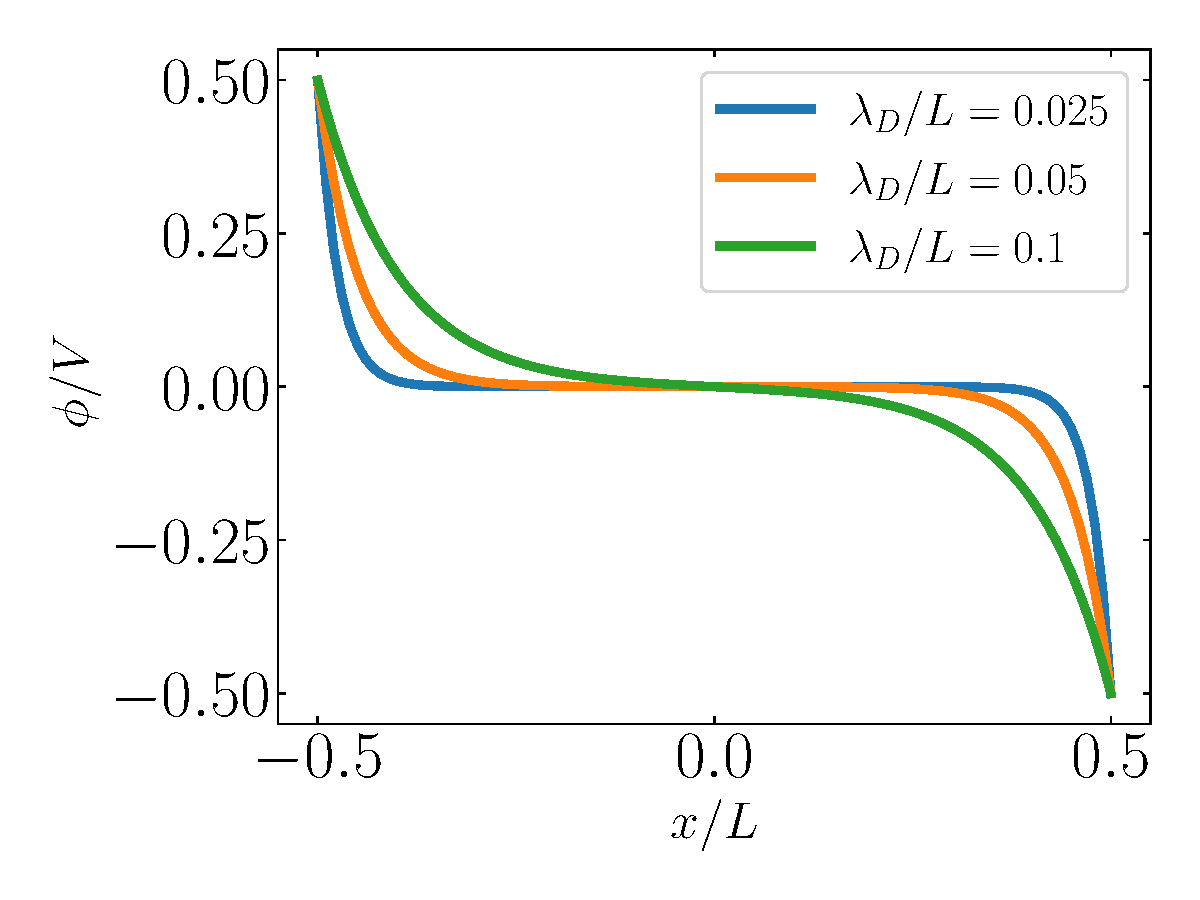
\includegraphics[width=\textwidth]{../../images/debye_phi.pdf}
        \caption{}
        \label{fig:debye_phi}
    \end{subfigure}
    \begin{subfigure}[b]{0.45\textwidth}
        \centering
        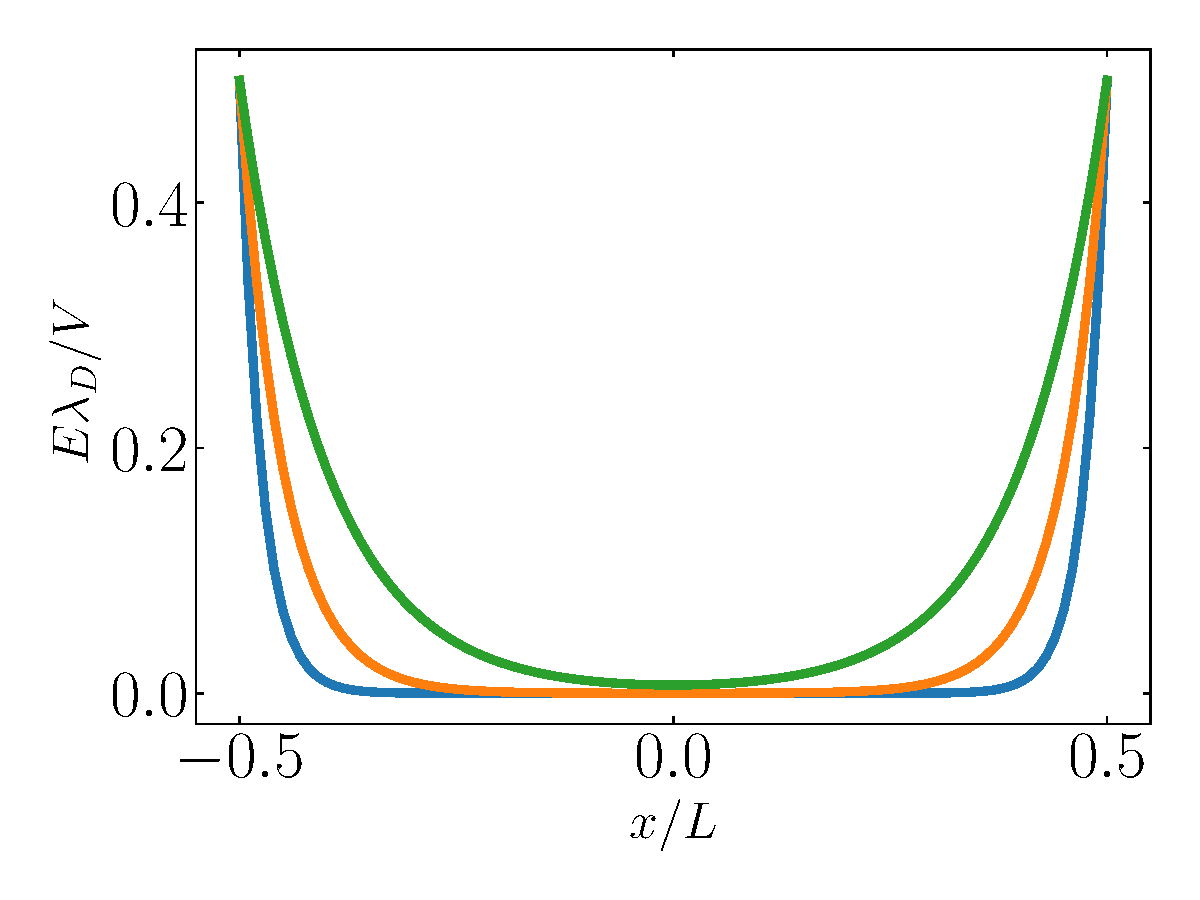
\includegraphics[width=\textwidth]{../../images/debye_elec.pdf}
        \caption{}
        \label{fig:debye_elec}
    \end{subfigure}
    \caption{Electric potential and field for various values of $\lambda_D/L$.}
    \label{fig:debye_phi_elec}
\end{figure}

We note that $\lambda_{De}$,  $w_{pe}$, and $v_{Te}$ are all related to each other as shown below
\begin{equation}
    \label{eq:debye_3vars}
    \lambda_{De} w_{pe} = \left ( \frac{\epsilon_0 k_B T_e}{n_{e0} e^2} \right )^{1/2} \left ( \frac{n_{e0} e^2}{m_e \epsilon_0} \right )^{1/2} = \left ( \frac{k_B T_e}{m_e} \right )^{1/2} = v_{Te}.
\end{equation}

%--------------------------------------------
\subsection{Plasma frequency}
%--------------------------------------------
We'll use the same setting as that for the derivation of the Debye length. The only difference is that the potential drop across the domain now oscillates with a frequency of $w$, that is $\phi_1(-L/2) - \phi_1(L/2) = V \exp (-iwt)$.

The starting point is \cref{eq:ep_waves_pre_dispersion}, that is, the equation for electron-plasma waves after assuming $n_{e1} = \tilde{n}_{e1} \exp (-i w t)$, where $\tilde{n}_{e1} = \tilde{n}_{e1}(\xvec)$. In one dimension this equation takes the form
\begin{equation*}
    \left ( w^2 - w_{pe}^2 \right ) n_{e1} + \gamma_e v_{Te}^2 \frac{d^2 n_{e1}}{dx^2} = 0.
\end{equation*}
Plugging in \cref{eq:ep_waves_efield_divergence} in the above and using the definition of the electric potential, we get
\begin{equation*}
    (w^2 - w_{pe}^2) \frac{d^2 \phi_1}{dx^2} + \gamma_e v_{Te}^2 \frac{d^4 \phi_1}{dx^4} = 0,
\end{equation*}
which we re-write as
\begin{equation*}
    \frac{d^4 \phi_1}{dx^4} + \frac{(w^2 - w_{pe}^2)}{\gamma_e v_{Te}^2} \frac{d^2 \phi_1}{dx^2} = 0.
\end{equation*}
Using \cref{eq:debye_3vars} the above becomes
\begin{equation*}
    \frac{d^4 \phi_1}{dx^4} + \frac{(w^2 - w_{pe}^2)}{\gamma_e (\lambda^2_{De} w^2_{pe}) } \frac{d^2 \phi_1}{dx^2} = 0,
\end{equation*}
or
\begin{equation*}
    \frac{d^4 \phi_1}{dx^4} + \frac{1}{\gamma_e \lambda^2_{De}} \left( \frac{w^2}{w^2_{pe}} - 1 \right) \frac{d^2 \phi_1}{dx^2} = 0.
\end{equation*}
Since we assumed electron number densities of the form $n_{e1} = \tilde{n}_{e1} \exp (-i w t)$, we choose $\phi_1 = \tilde{\phi}_1 \exp(-iwt)$, where $\tilde{\phi}_1 = \tilde{\phi}_1(x)$, so as to satisfy \cref{eq:ep_waves_efield_divergence}. Thus, we get
\begin{equation*}
    \frac{d^4 \tilde{\phi}_1}{dx^4} + \frac{1}{\gamma_e \lambda^2_{De}} \left( \frac{w^2}{w^2_{pe}} - 1 \right) \frac{d^2 \tilde{\phi_1}}{dx^2} = 0.
\end{equation*}
Integrating twice we get 
\begin{equation*}
    \frac{d^2 \tilde{\phi}_1}{dx^2} + \frac{1}{\gamma_e \lambda^2_{De}} \left( \frac{w^2}{w^2_{pe}} - 1 \right) \tilde{\phi_1} + C_1 x + C_2 = 0.
\end{equation*}
We only have one boundary condition, namely $\phi_1(-L/2) - \phi_1(L/2) = V \exp (-iwt)$, yet the equation for $\phi$ is originally of fourth order. Thus, we prescribe additional boundary conditions such that $C_1 = C_2 = 0$. The equation for $\tilde{\phi}$ then is simply
\begin{equation}
    \label{eq:params_pf_ode_general}
    \frac{d^2 \tilde{\phi}_1}{dx^2} + \frac{1}{\gamma_e \lambda^2_{De}} \left( \frac{w^2}{w^2_{pe}} - 1 \right) \tilde{\phi_1} = 0.
\end{equation}

\subsubsection{Case 1 $w_{pe} \le w$}
We introduce the variable $\alpha$ so that it satisfies
\begin{equation}
    \frac{1}{\alpha^2} = \frac{1}{\gamma_e \lambda^2_{De}} \left( \frac{w^2}{w^2_{pe}} - 1 \right).
\end{equation}
Note that $\alpha$ is always positive. \Cref{eq:params_pf_ode_general} becomes 
\begin{equation}
    \frac{d^2 \tilde{\phi}_1}{dx^2} + \frac{1}{\alpha^2} \tilde{\phi}_1 = 0,
\end{equation}
The general solution to the above is
\begin{equation*}
    \tilde{\phi}_1 = c_1 \exp (i x / \alpha) + c_2 \exp (-i x / \alpha).
\end{equation*}
We introduce a new boundary condition, namely $\tilde{\phi}_1(0) = 0$, which gives $c_2 = -c_1$. Thus, the solution takes the form
\begin{equation*}
    \tilde{\phi}_1 = c_1 \left[ \exp (i x / \alpha) - \exp (-i x / \alpha) \right] = c_1 2i \sin ( x / \alpha ).
\end{equation*}
Applying the other boundary condition for $\tilde{\phi}$, namely, $\tilde{\phi}_1(-L/2) - \tilde{\phi}_1(L/2) = V$, we get
\begin{equation*}
    c_1 2i \left[ -\sin \left( L / 2\alpha \right) - \sin \left( L / 2\alpha \right) \right] = V,
\end{equation*}
or
\begin{equation*}
    c_1 = - \frac{V}{4i \sin \left( L / 2\alpha \right)}.
\end{equation*}
Thus, the final solution for $\phi_1$ is
\begin{equation}
    \phi_1 = - \frac{V}{2} \frac{\sin (x / \alpha)}{\sin (L / 2\alpha)} \exp(-iwt).
\end{equation}

\subsubsection{Case 2 $w_{pe} \ge w$}
We introduce the variable $\beta$ so that it satisfies
\begin{equation}
    \frac{1}{\beta^2} = \frac{1}{\gamma_e \lambda^2_{De}} \left( 1 - \frac{w^2}{w^2_{pe}} \right).
\end{equation}
Note that $\beta$ is always positive. \Cref{eq:params_pf_ode_general} becomes 
\begin{equation}
    \frac{d^2 \tilde{\phi}_1}{dx^2} - \frac{1}{\beta^2} \tilde{\phi}_1 = 0,
\end{equation}
The general solution to the above is
\begin{equation*}
    \tilde{\phi}_1 = c_1 \exp (x / \beta) + c_2 \exp (-x / \beta).
\end{equation*}
As before, we use the boundary condition $\tilde{\phi}_1(0) = 0$, which gives $c_2 = -c_1$. Thus, the solution takes the form
\begin{equation*}
    \tilde{\phi}_1 = c_1 \left[ \exp (x / \beta) - \exp (-x / \beta) \right] = c_1 2 \sinh (x / \beta).
\end{equation*}
Applying the other boundary condition for $\tilde{\phi}$, namely, $\tilde{\phi}_1(-L/2) - \tilde{\phi}_1(L/2) = V$, we get
\begin{equation*}
    c_1 2 \left[ -\sinh \left( L / 2 \beta \right) - \sinh \left( L / 2 \beta \right) \right] = V,
\end{equation*}
or
\begin{equation*}
    c_1 = - \frac{V}{4 \sin \left( L / 2 \beta \right)}.
\end{equation*}
Thus, the final solution for $\phi_1$ is
\begin{equation}
    \phi_1 = - \frac{V}{2} \frac{\sinh (x / \beta)}{\sinh (L / 2 \beta)} \exp(-iwt).
\end{equation}
Note that the spatial functional form of the above is equivalent to \cref{eq:debye_phi_sol} if $\beta$ were to be equal to $\lambda_D$.

Add some plots to visualize cases 1 and 2.

It is often important to know the plasma density at which the electron plasma frequency $w_{pe}$ equals the external frequency $w$. This density is referred to as the critical density $n_{cr}$. Equating the electron plasma frequency with the external frequency we get
\begin{equation*}
    \frac{n_{cr} e^2}{m_e \epsilon_0} = w^2,
\end{equation*}
which leads to
\begin{equation}
    \label{eq:plas_freq_crit_den}
    n_{cr} = \frac{m_e \epsilon_0 w^2}{e^2}
\end{equation}
The above can be re-written as
\begin{equation*}
    n_{cr} = \frac{m_e \epsilon_0 (2 \pi \nu)^2}{e^2} = \frac{4 \pi^2 m_e \epsilon_0 c^2}{e^2} \frac{1}{\lambda^2} = 1.115 \times 10^{27} \frac{1}{\lambda_{\mu m}^2},
\end{equation*}
where $\lambda_{\mu m}$ is in units of microns and $n_{cr}$ in units of \#/m\textsuperscript{3}.

%--------------------------------------------
\subsection{The coupling parameter}
%--------------------------------------------

Coulomb interactions are those which occur when two charge particles head towards each other. We can define two types of Coulomb interactions: strong and weak. Strong Coulomb interactions are those for which the particle's Coulomb potential energy is larger than its kinetic energy, and vice versa for weak Coulomb interactions. Thus, we can also define two types of plasma regimes:
\begin{itemize}
    \item Strongly-coupled plasmas: plasmas where the Coulomb interactions are mostly strong and thus drive the dynamics of its evolution. Coulomb interactions tend to be strong when the inter-particle distances are small, and thus this regime would be dominated by \textit{short-range} interactions. These plasmas are also described as exhibiting \textit{collisional} behavior, since a strong Coulomb interaction essentially means a collision has occurred.
    \item Weakly-coupled plasmas: plasmas where the Coulomb interactions are mostly weak, and as a result do not drive the dynamics of its evolution. The plasma dynamics are instead driven by \textit{long-range} effects caused by smooth electromagnetic fields that result from integrating a large number of particles. These plasmas are also described as exhibiting \textit{collective} behavior, since the long-range electromagnetic fields follow from the collective integration of many particles.
\end{itemize}

We describe an approximate Coulomb potential energy for particles in a plasma as
\begin{equation}
    U =  \frac{q_s^2}{4 \pi \epsilon_0 a_s}.
\end{equation}
The impact parameter that has been used above is $a_s$, the sphere radius. This provides a decent measure on the average spacing between particles in a plasma. Since the volume of a single particle is $1/n_s$, and if we assume that this volume is given by $4/3 \pi a_s^3$, then equating these two gives the expression for the sphere radius
\begin{equation}
    a_s = \left ( \frac{3}{4 \pi n_s} \right )^{1/3}.
\end{equation}
The thermal velocity of a particle is given by
\begin{equation}
    v_{T_s} = \sqrt{\frac{k_B T_s}{m_s}}
\end{equation}
A measure of the kinetic energy of a particle is given in terms of the thermal velocity as shown below
\begin{equation}
    K = m_s v_{T_s}^2 = k_B T_s
\end{equation}
The ratio of the particle's Coulomb potential energy and its kinetic energy is referred to as the coupling parameter $\Gamma_s$. That is 
\begin{equation}
    \Gamma_s = \frac{q_s^2}{4 \pi \epsilon_0 a_s k_B T_s}.
\end{equation}
$\Gamma_s > 1$ denotes a strongly coupled plasma, and $\Gamma_s < 1$ denotes a weakly coupled plasma. 

%--------------------------------------------
\subsection{The plasma parameter}
%--------------------------------------------
The standard plasma parameter $\Lambda_s$ is defined as
\begin{equation}
    \Lambda_s = \frac{4}{3} \pi \lambda_{Ds}^3 n_s.
\end{equation}

There is a one to one relationship between the coupling parameter and the standard plasma parameter. Simple algebra shows that 
\begin{equation}
    \Gamma_s = (1/3) \Lambda_s^{-2/3}.
\end{equation}
Thus, the coupling and plasma parameters are inversely proportional to each other. $\Lambda_s < 1$ implies strongly-coupled plasmas, and $\Lambda_s > 1$ weakly-coupled plasmas. Since $\Lambda_s$ represents the number of particles per Debye sphere, it is interesting to see that a large number of particles within such a sphere is needed to be in the weakly-coupled-plasma regime. However, this does not correspond to a plasma with large density, in fact, it corresponds to the opposite. The explicit $n_s$ term in the definition $\Lambda_s = (4/3) \pi \lambda^3_{Ds} n_s$ is dominated by the $n_s$ in the denominator of $\lambda_{Ds}$. In other words, low plasma densities lead to large Debye spheres, which in turn leads to many particles per Debye sphere, and hence a weakly-coupled plasma.

%--------------------------------------------
\subsection{Electron degeneracy}
%--------------------------------------------

\begin{itemize}
    \item DeBroglie wavelength
    \begin{equation}
        \lambda_{Bs} = \dfrac{h}{\sqrt{2 \pi} m_s v_{Ts}}
    \end{equation}
    \item Quantum plasma parameter
    \begin{equation}
        \chi_s = \frac{4}{3} \pi \lambda_{Bs}^3 n_s
    \end{equation}
    
    \item Fermi energy:
    \begin{equation}
        E_{fs} = \frac{\hbar^2}{2m_s} \left ( 3 \pi^2 n_s \right)^{2/3}
    \end{equation}

    \item The Fermi energy can be used to define the Fermi temperature $T_{fs}$, Fermi velocity $v_{fs}$, Fermi momentum $p_{fs}$, and Fermi wave vector $k_{fs}$
    \begin{equation}
        E_{fs} = k_B T_{fs} = \frac{1}{2} m_s v_{fs}^2  = \frac{p_{fs}^2}{2m_s} = \frac{\left ( \hbar k_{fs} \right ) ^2}{2m_s}
    \end{equation}

    \item Degeneracy parameter:
    \begin{equation}
        \Theta_s = \frac{k_B T_s}{E_{fs}} = \left( \frac{2^{10} \pi}{3^4} \right)^{1/3} \chi_s^{-2/3}.
    \end{equation}
\end{itemize}

%########################################################################
\chapter{Collisions}
%########################################################################
%------------------------------------------------------------------------
\section{Cross section}
%------------------------------------------------------------------------
%--------------------------------------------
\subsection{General definition}
%--------------------------------------------
Two particles traveling towards each other can undergo an interaction. Types of interactions include Coulomb collisions between two charged particles, fusion reactions between ions, and photon-matter phenomena such as Compton scattering, the photoelectric effect, and pair production.

\begin{figure}[ht]
    \centering
    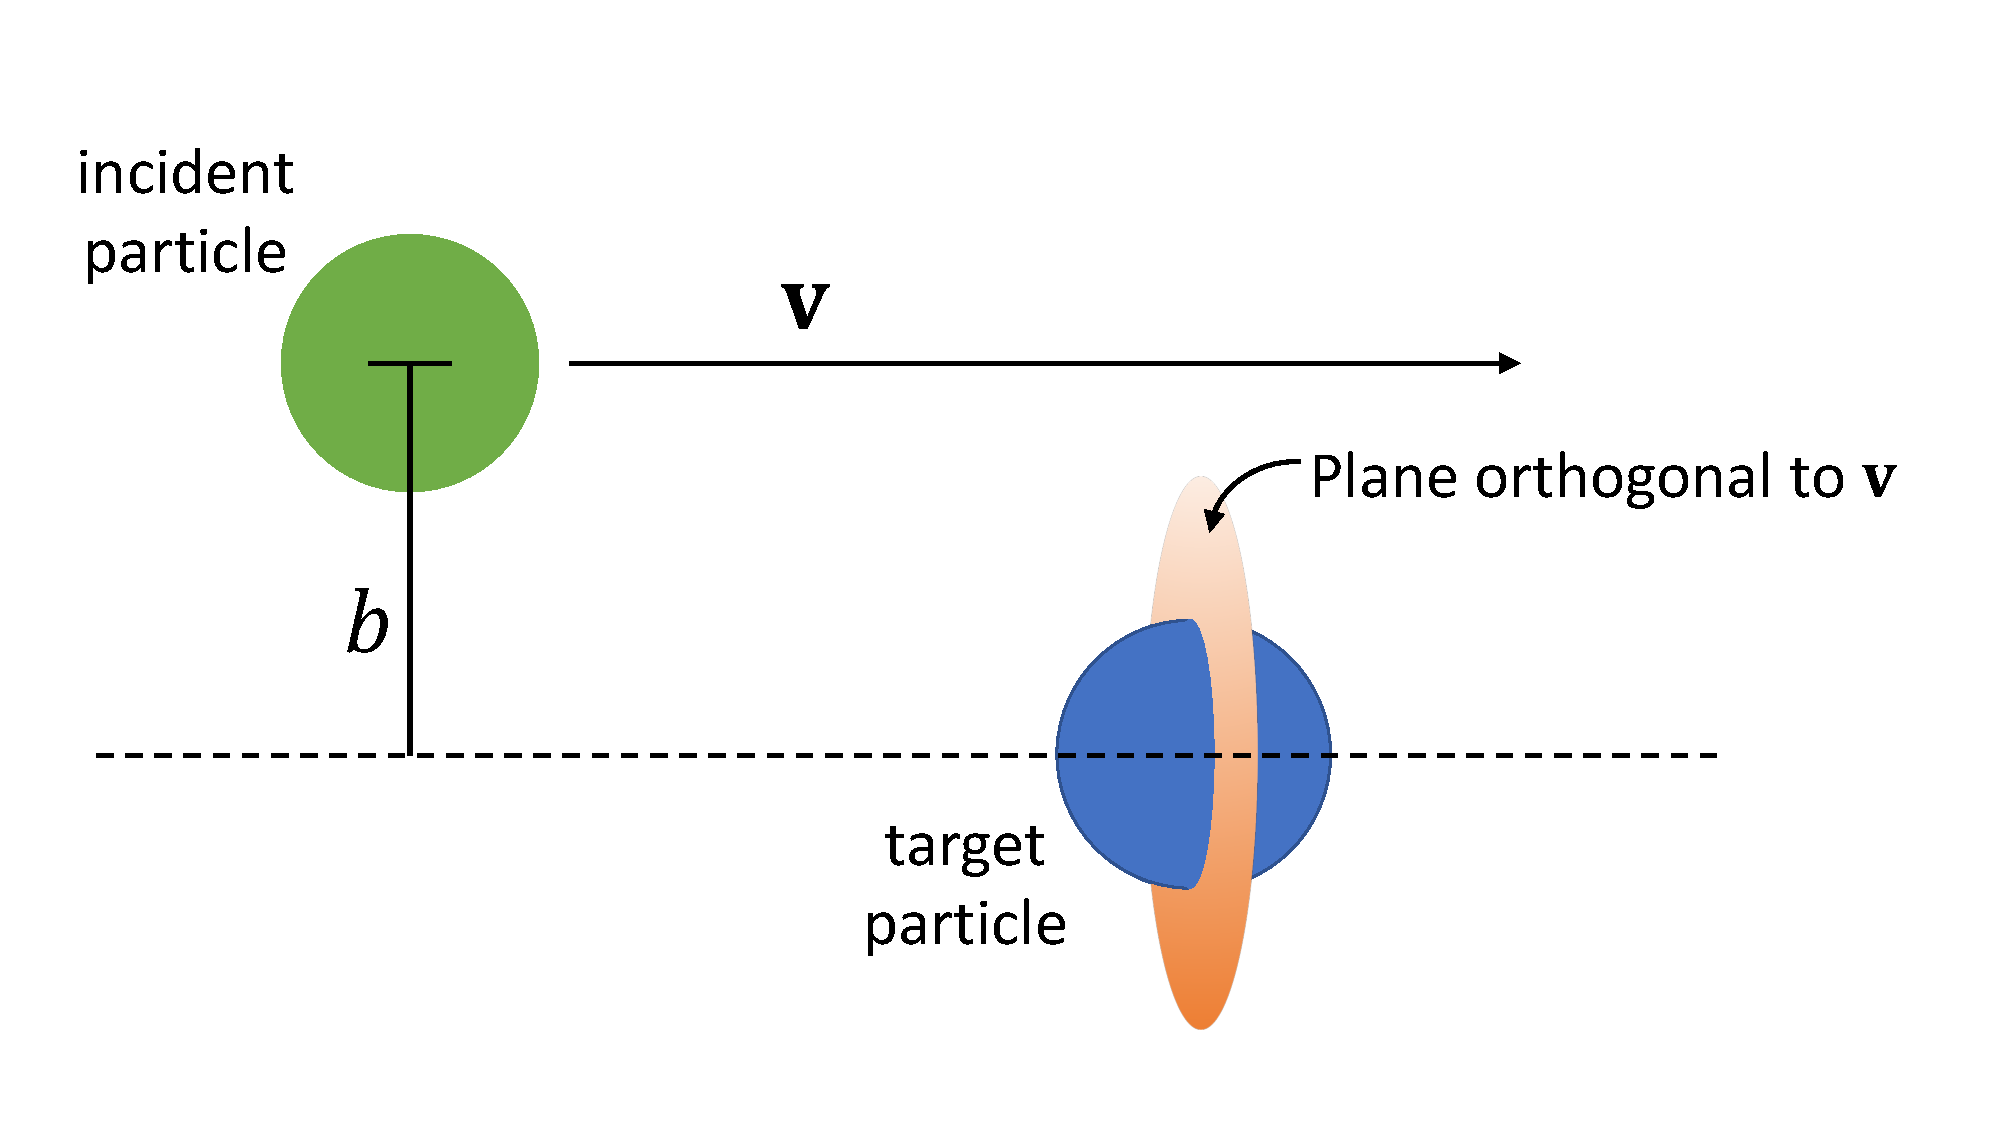
\includegraphics[width=10cm]{../../images/cross_section.pdf}
    \caption{Interaction of incident and target particles.}
    \label{fig:cross_many_particles}
\end{figure}
To define the cross section, we'll consider $I$ incident particles heading towards $J$ stationary target particles (see \cref{fig:cross_many_particles}). Not all of the incident particles will interact with the target particles, some will instead continue to travel in a uniform trajectory. The number of incident particles that do interact with the target particles is labeled as $N$. The cross section $\sigma$ is then a constant of proportionality defined by the following equation
\begin{equation}
    \label{eq:cross_def}
    N = \sigma I n_A.
\end{equation}
In the above, $n_A$ is the areal number density, that is, $n_A = J / A = n \Delta x$, where $n$ is the volume number density.

%--------------------------------------------
\subsection{Differential cross section}
%--------------------------------------------
\begin{figure}[ht]
    \centering
    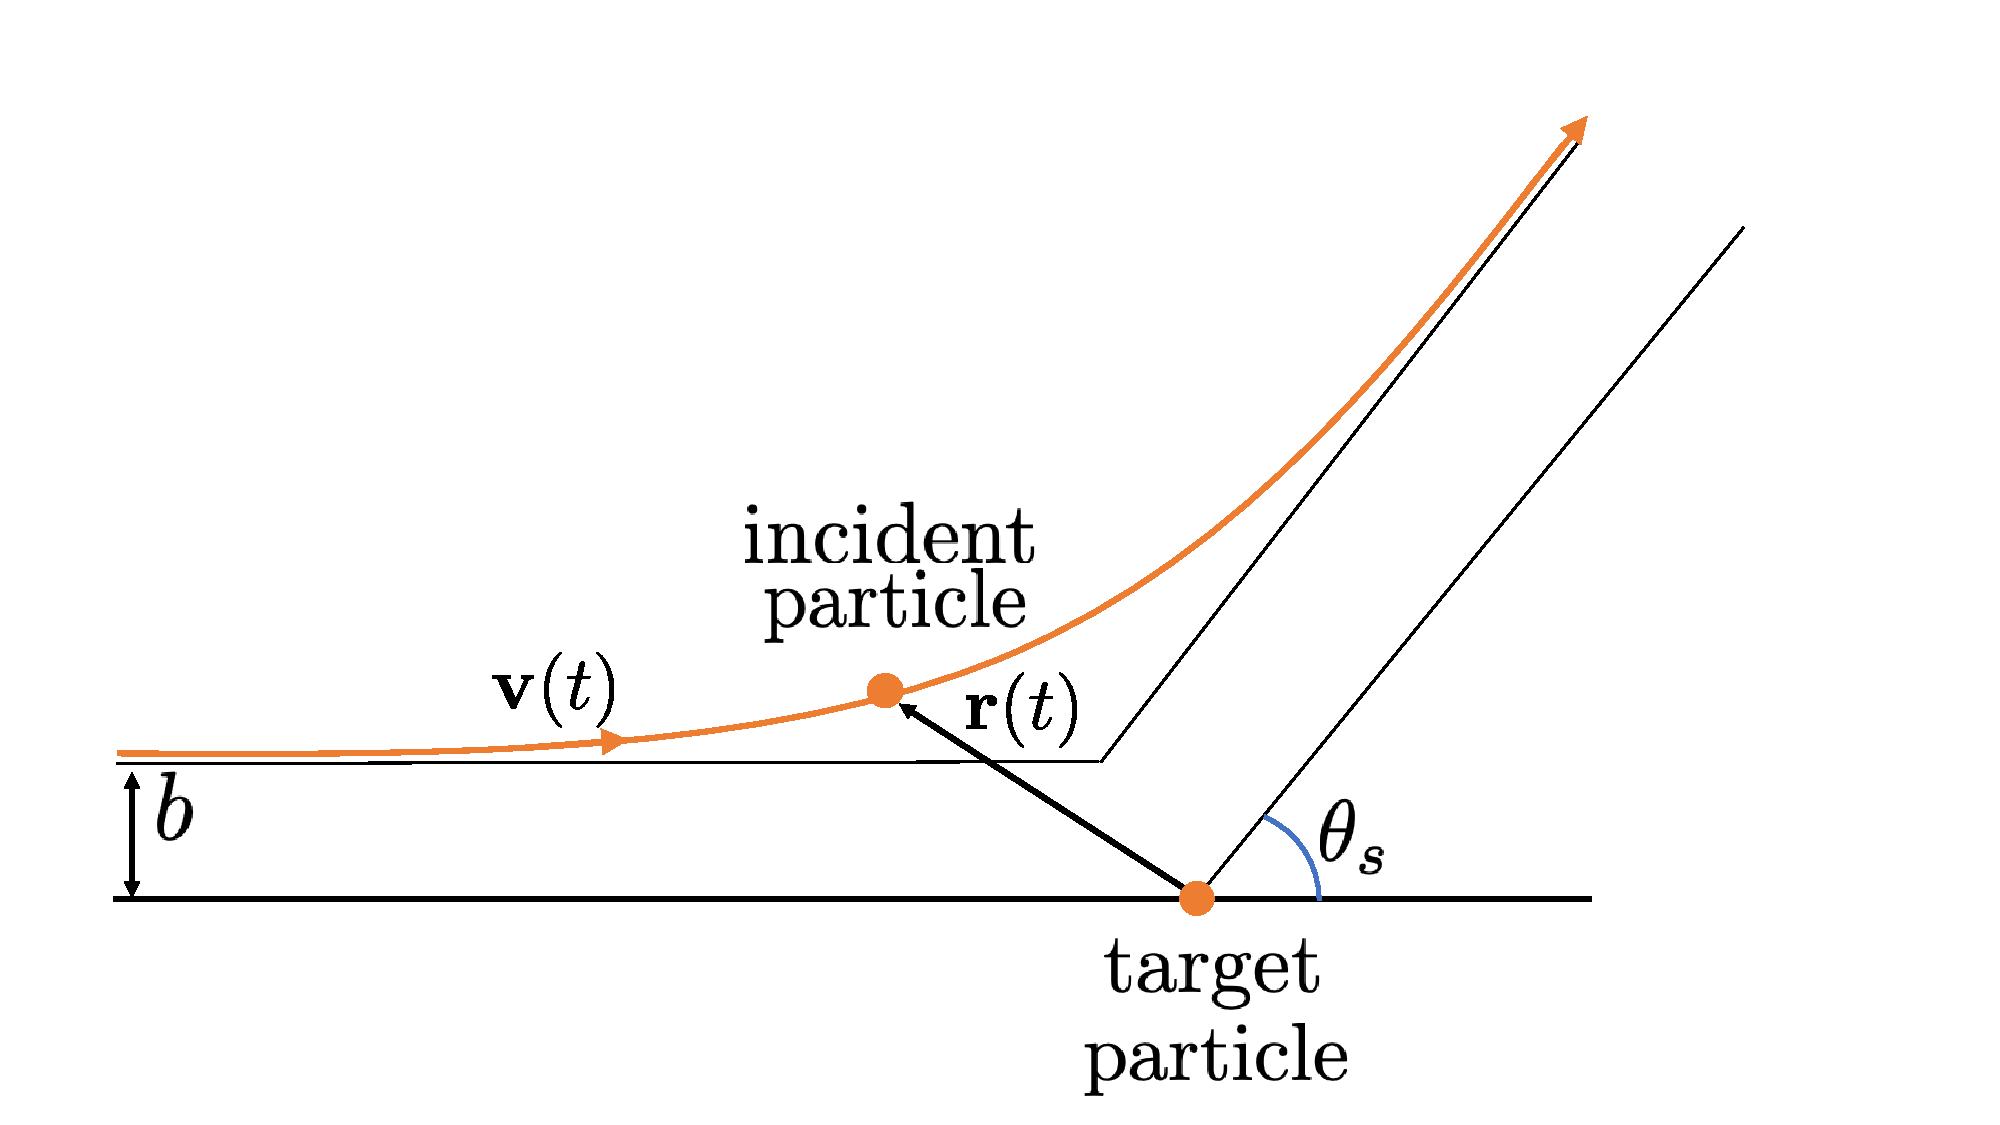
\includegraphics[width=10cm]{../../images/scattering.pdf}
    \caption{Depiction of particle scattering.}
    \label{fig:scattering}
\end{figure}

Consider the scattering of two particles: an incident and a target particle. If we fix the reference frame to follow the target particle, then the scattering can be depicted as shown in \cref{fig:scattering}. The displacement parameter is labelled as $b$, and the scattering angle as $\theta_s$. For three dimensional scattering, the encounter is as shown in \cref{fig:scattering_3d}. Not that in that figure the incident particle starts within the $x-z$ plane, and after scattering the particle is confined to a plane that is tilted an angle $\phi_s$ from the $x-z$ plane.

\begin{figure}[ht]
    \centering
    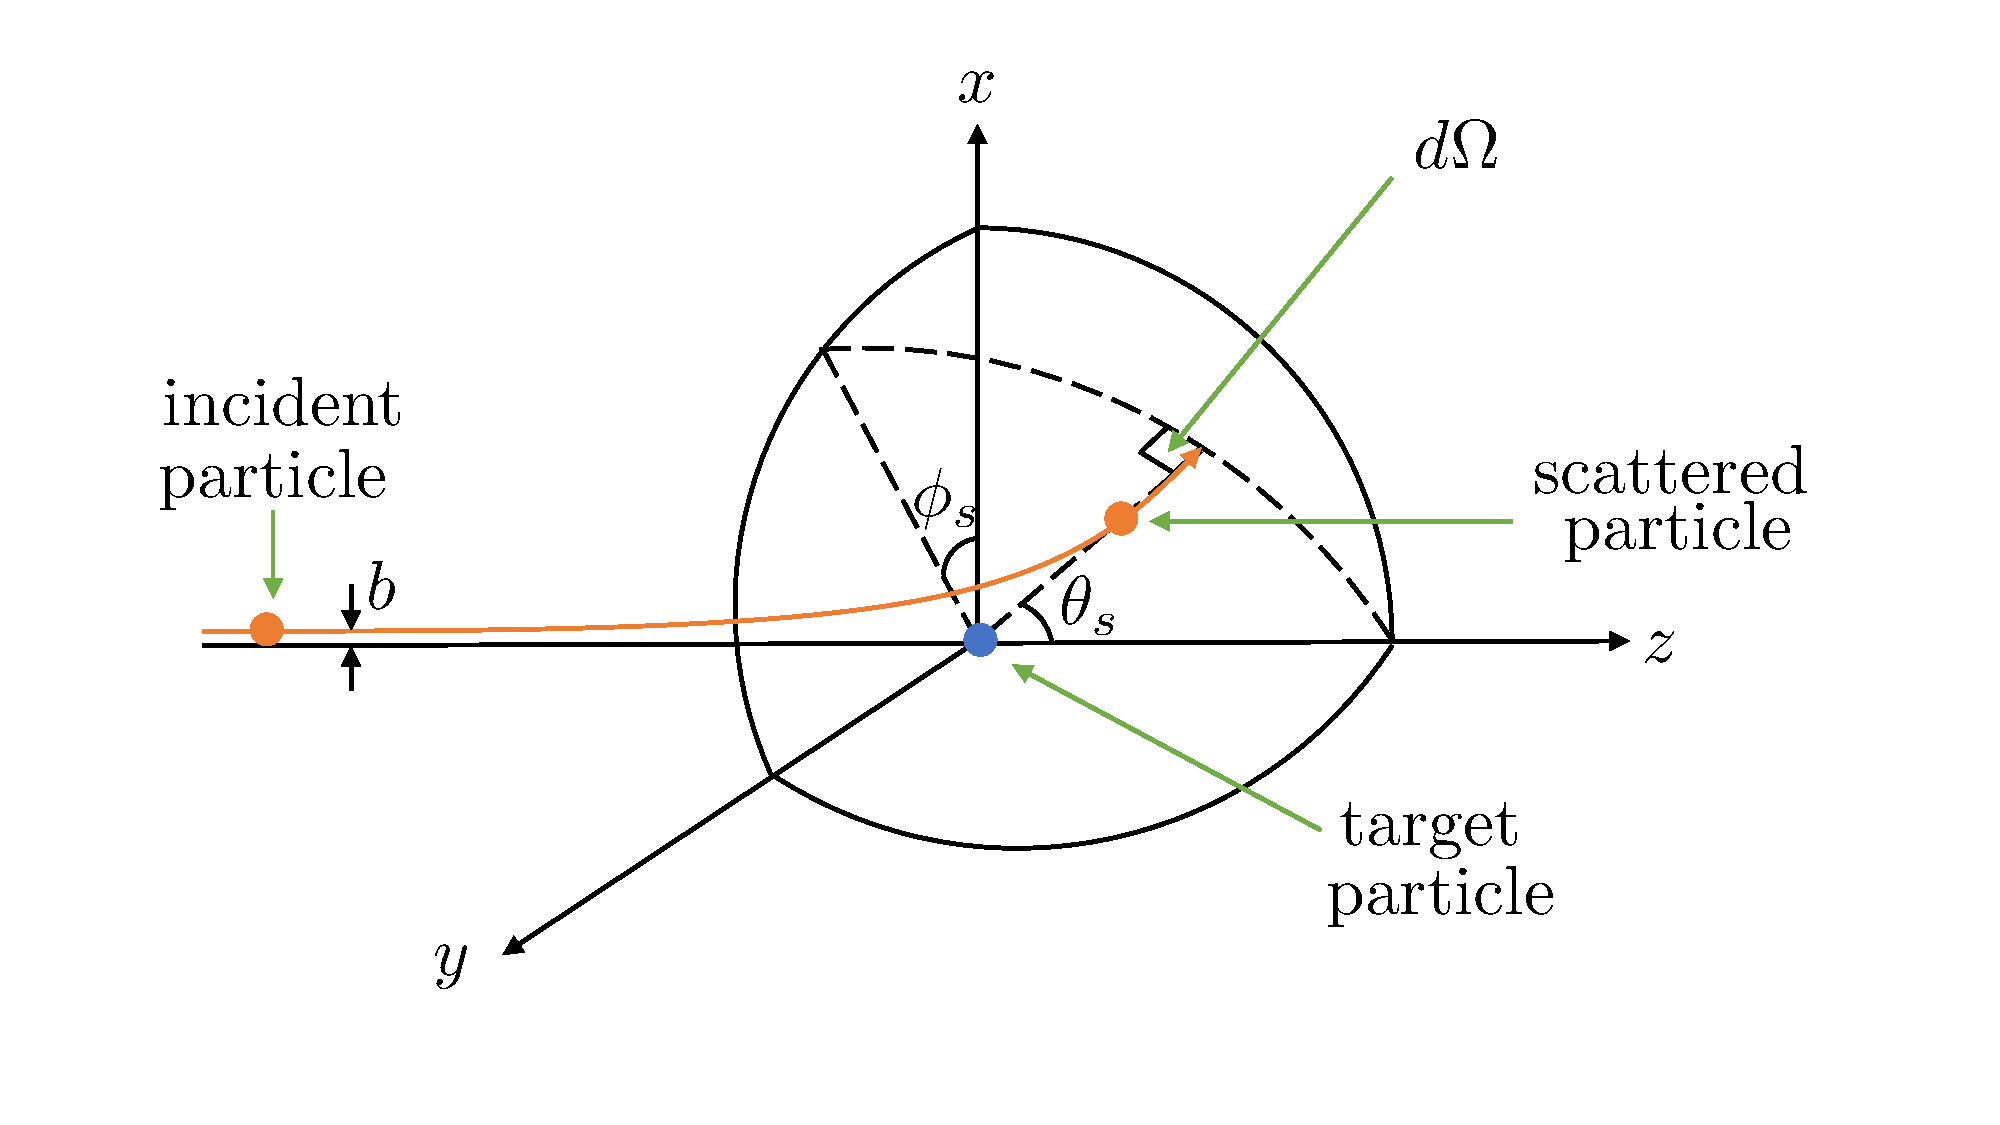
\includegraphics[width=10cm]{../../images/scattering_3d.pdf}
    \caption{Depiction of particle scattering in 3D.}
    \label{fig:scattering_3d}
\end{figure}

From the entire set of incident particles $N$ that interact with the target particles, one can define an infinitesimal subset $N_{\theta,\phi} d\Omega$ as the number of particles scattered into an infinitesimal solid angle $d\Omega = \sin \theta_s d\theta_s d\phi_s$, as shown in \cref{fig:scattering_3d}. We note that $N_{\theta,\phi} = N_{\theta,\phi} (\theta_s, \phi_s)$. We introduce the differential cross section
\begin{equation}
    \frac{d\sigma_{\theta,\phi}}{d\Omega} = \frac{d\sigma_{\theta,\phi}}{d\Omega}(\theta_s,\phi_s),
\end{equation}
which is defined by the following expression in an analogous manner to \cref{eq:cross_def},
\begin{equation}
    \label{eq:cross_def_diff}
    N_{\theta, \phi} d\Omega = \left ( \frac{d\sigma_{\theta,\phi}}{d\Omega} d\Omega \right ) I n_A.
\end{equation}
It is best to not think of it as a derivative (what does a derivative with respect to solid angle mean?) and instead to simply think of it as a function that depends on $\theta_s$ and $\phi_s$. Integrating over all $\theta_s$ and $\phi_s$, i.e.
\begin{equation*}
    \int_{\theta_s = 0}^\pi \int_{\phi_s = 0}^{2\pi} N_{\theta, \phi} d\Omega = \int_{\theta_s = 0}^\pi \int_{\phi_s = 0}^{2\pi} \frac{d\sigma_{\theta,\phi}}{d\Omega}  d\Omega I n_A
\end{equation*}
gives \cref{eq:cross_def}.

\begin{figure}[ht]
    \centering
    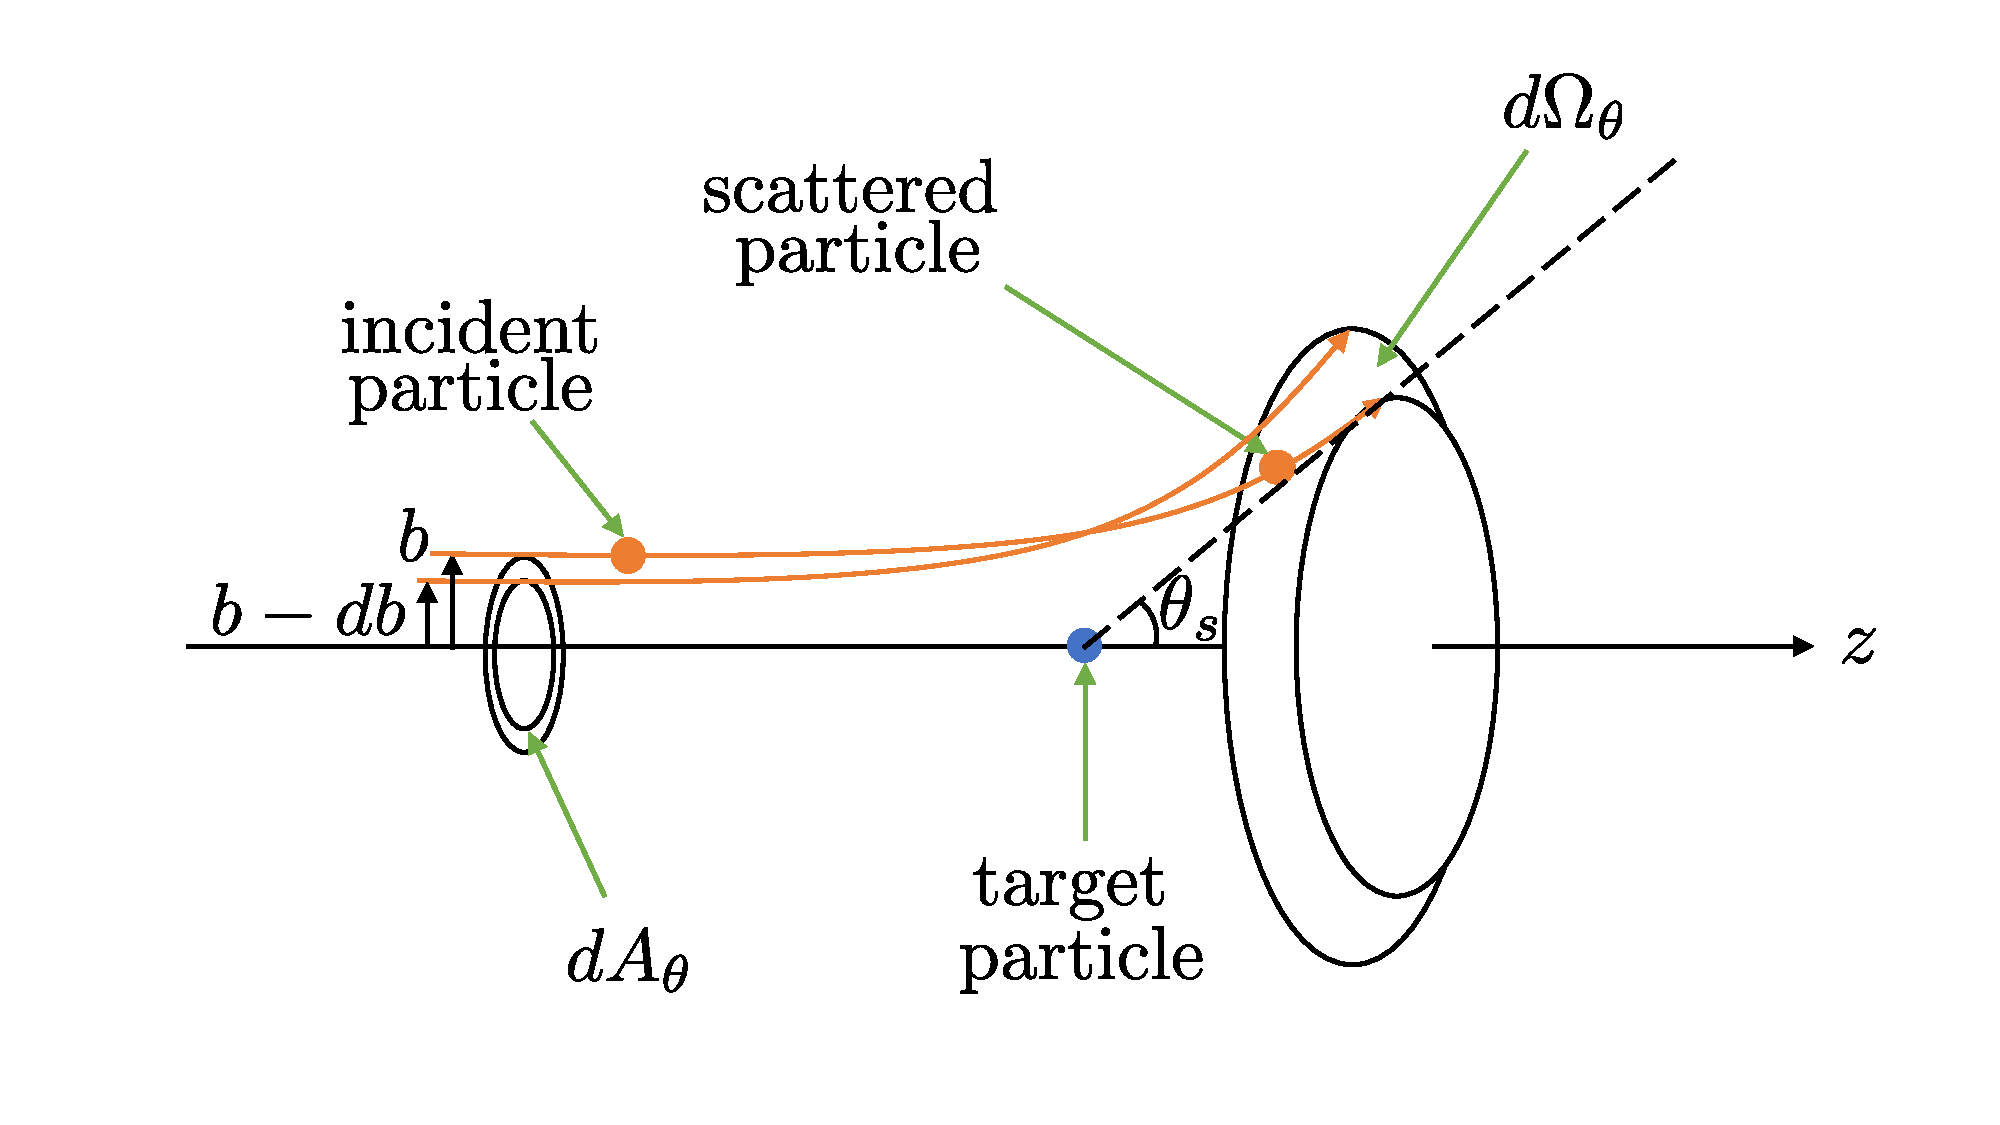
\includegraphics[width=10cm]{../../images/scattering_axi.pdf}
    \caption{Depiction of particle scattering in for axi-symmetric interactions.}
    \label{fig:scattering_axi}
\end{figure}
For various cases the scattering is axi-symmetric, that is, it is independent of $\phi_s$. Thus
\begin{equation*}
    N_{\theta, \phi} \to N_\theta \qquad \frac{d\sigma_{\theta,\phi}}{d\Omega} \to \frac{d\sigma_\theta}{d\Omega},
\end{equation*}
where 
\begin{equation*}
    N_\theta = N_\theta (\theta_s),
\end{equation*}
and
\begin{equation*}
    \frac{d\sigma_\theta}{d\Omega} = \frac{d\sigma_\theta}{d\Omega} (\theta_s).
\end{equation*}
Integrating \cref{eq:cross_def_diff} from $\phi_s = 0$ to $\phi_s = 2\pi$ gives
\begin{equation}
    \label{eq:cross_def_diff_axi}
    N_\theta d\Omega_\theta = \frac{d\sigma_\theta}{d\Omega} d\Omega_\theta I n_A,
\end{equation}
where $d \Omega_\theta = 2\pi \sin \theta_s d\theta_s$. $N_\theta d\Omega_\theta$ thus represents the number of particles that are scattered into the infinitesimal band $d\Omega_\theta$ on a sphere, where $d\Omega_\theta$ is defined by scattering angle $\theta_s$ (see \cref{fig:scattering_axi}). We will note that there is a one-to-one correspondence between the impact parameter $b$ and the scattering angle $\theta_s$, that is, $b = b(\theta_s)$. In other words, any incident particle scattered out through the infinitesimal band $d\Omega_\theta$ would have approached the target-particle through the infinitesimal ring $dA_\theta$ that corresponds to $d\Omega_\theta$. Since there are many target particles, there are many $dA_\theta$'s that correspond to the same $d\Omega_\theta$. Thus, the total number of particles scattered through $d\Omega_\theta$ is given by all the incident particles that cross through the $dA_\theta$'s of all the target particles.

The number of incident particles crossing all the infinitesimal rings $dA_\theta$ is equal to the total number of incident particles $I$ times the probability $P$ that any single incident particle will cross one of those rings. Thus, we can write
\begin{equation*}
    N_\theta d\Omega_\theta = I P.
\end{equation*}
The probability that an incident particle will cross one of those rings is simply the ratio of the surface area covered by all the rings in a section of the target material to the total area of that section. The surface area covered by all the rings in a section of area $S$ is given by $(n_A S) dA_\theta$. Thus, $P = n_A dA_\theta$ and 
\begin{equation*}
    N_\theta d\Omega_\theta = I n_A dA_\theta.
\end{equation*}
We now introduce the differential 
\begin{equation}
    \label{eq:cross_impact_differential}
    db = \frac{db}{d\theta_s} d\theta_s.
\end{equation}
We note that by definition $d\theta_s$ is positive but $db$ can be either positive or negative depending on the sign of $db/d\theta_s$. The infinitesimal area $dA_\theta$ is then given by 
\begin{equation}
    \label{eq:cross_impact_area}
    dA_\theta= 2\pi b |db| = 2 \pi b \left | \frac{db}{d\theta_s} \right | d \theta_s.
\end{equation}
Thus, 
\begin{equation*}
    N_\theta d\Omega_\theta = n_A I 2 \pi b \left | \frac{db}{d\theta_s} \right | d \theta_s.
\end{equation*}
Using \cref{eq:cross_def_diff_axi} in the above, we get
\begin{equation*}
    \frac{d\sigma_\theta}{d\Omega} d\Omega_\theta I n_A = I n_A 2 \pi b \left | \frac{db}{d\theta_s} \right | d \theta_s, 
\end{equation*}
or 
\begin{equation}
    \label{eq:cross_diff_impact_axi}
    \frac{d\sigma_\theta}{d\Omega} = \frac{b}{\sin \theta_s} \left | \frac{db}{d\theta_s} \right |.
\end{equation}

%--------------------------------------------
\subsection{Mean free path \& collision frequency}
%--------------------------------------------
The mean free path can be expressed in terms of the cross section as
\begin{equation}
    \lambda_m = \frac{1}{n_1 \sigma}.
\end{equation}
Given the particle's speed $v$, on can also define the collision time as follows
\begin{equation}
    \tau_m = \frac{\lambda_m}{v} = \frac{1}{n_1 \sigma v}.
\end{equation}
Finally, the collision frequency is simply the inverse of the collision time, that is
\begin{equation}
    \nu_{m} = \frac{1}{\tau_m} = n_1 \sigma v.
\end{equation}

%------------------------------------------------------------------------
\section{Coulomb collisions}
%------------------------------------------------------------------------

%--------------------------------------------
\subsection{Particle equations}
%--------------------------------------------
\label{sec:coulomb_particle_equations}
Consider two particles, with positions $\rvec_1=\rvec_1(t)$ and $\rvec_2=\rvec_2(t)$, velocities $\vvec_1=\vvec_1(t)$ and $\vvec_2=\vvec_2(t)$, charges $q_1$ and $q_2$, and masses $m_1$ and $m_2$, respectively. Their positions and velocities are governed by the following equations 
\begin{equation}
    \label{eq:coul_particle_1_pos}
    \frac{d \rvec_1}{dt} = \vvec_1,
\end{equation}
\begin{equation}
    \label{eq:coul_particle_2_pos}
    \frac{d \rvec_2}{dt} = \vvec_2,
\end{equation}
\begin{equation}
    \label{eq:coul_particle_1_vel}
    m_1 \frac{d\vvec_1}{dt} = -\frac{q_1 q_2}{4 \pi \epsilon} \frac{\rvec_2 - \rvec_1}{\left | \rvec_2 - \rvec_1 \right |^3},
\end{equation}
\begin{equation}
    \label{eq:coul_particle_2_vel}
    m_2 \frac{d\vvec_2}{dt} = -\frac{q_1 q_2}{4 \pi \epsilon} \frac{\rvec_1 - \rvec_2}{\left | \rvec_1 - \rvec_2 \right |^3}.
\end{equation}
We note that the above system consists of twelve equations for twelve unknowns. We now introduce the center-of-mass position $\Rvec = \Rvec(t)$, the center-of-mass velocity $\Vvec = \Vvec(t)$, the shifted position $\rvec = \rvec(t)$ and the shifted velocity $\vvec = \vvec(t)$ as follows
\begin{equation*}
    \Rvec = \frac{m_1 \rvec_1 + m_2 \rvec_2}{m_1 + m_2} \qquad \rvec = \rvec_1 - \rvec_2,
\end{equation*}
\begin{equation*}
    \Vvec = \frac{m_1 \vvec_1 + m_2 \vvec_2}{m_1 + m_2} \qquad \vvec = \vvec_1 - \vvec_2
\end{equation*}
Thus, in terms of these new four variables, the particle equations can be written as
\begin{equation}
    \frac{d \Rvec}{dt} = \Vvec,
\end{equation}
\begin{equation}
    \frac{d \Vvec}{dt} = 0 ,
\end{equation}
\begin{equation}
    \label{eq:particle_pos}
    \frac{d \rvec}{dt} = \vvec,
\end{equation}
\begin{equation}
    \label{eq:coul_particle_vel}
    \frac{d \vvec}{dt} = \frac{q_1 q_2}{4\pi \epsilon_0 m_r} \frac{\rvec}{r^3},
\end{equation}
where the reduced mass $m_r$ is given by
\begin{equation}
    \label{eq:coul_reduced_mass}
    \frac{1}{m_r} = \frac{1}{m_1} + \frac{1}{m_2}.
\end{equation}
The first two equations above give the trivial solution $\Vvec = $ constant and $\Rvec$ = $\Rvec(0) + \Vvec t$. Thus, we have reduced the problem from twelve unknowns to six unknowns, namely $\rvec$ and $\vvec$.

%--------------------------------------------
\subsection{Conservation of energy and momentum}
%--------------------------------------------
Dotting \cref{eq:coul_particle_vel} by $\vvec$ gives 
\begin{align*}
    \vvec \cdot \frac{d \vvec}{dt} &= \frac{q_1 q_2}{4 \pi \epsilon_0 m_r} \vvec \cdot \frac{\rvec}{r^3} \nonumber \\
    &= \frac{q_1 q_2}{4 \pi \epsilon_0 m_r} \frac{d\rvec}{dt} \cdot \frac{\rvec}{r^3} \nonumber \\
    &= \frac{q_1 q_2}{4 \pi \epsilon_0 m_r} \frac{1}{2} \frac{dr^2}{dt} \frac{1}{r^3} \nonumber \\
    &= \frac{q_1 q_2}{4 \pi \epsilon_0 m_r} \frac{1}{r^2} \frac{dr}{dt} \nonumber \\
    &= -\frac{q_1 q_2}{4 \pi \epsilon_0 m_r} \frac{d}{dt} \left ( \frac{1}{r} \right ).
\end{align*} 
For the left hand side above we have
\begin{equation*}
    \vvec \cdot \frac{d \vvec}{dt} = \frac{1}{2} \frac{d v^2}{dt},
\end{equation*}
and thus we obtain the following expression for conservation of energy
\begin{equation*}
    \frac{d}{dt} \left ( \frac{1}{2} m_r v^2 + \frac{q_1 q_2}{4 \pi \epsilon_0} \frac{1}{r} \right ) = 0.
\end{equation*}

Crossing \cref{eq:coul_particle_vel} by $\rvec$ gives
\begin{equation*}
    \rvec \times \frac{d \vvec}{dt} = \frac{q_1 q_2}{4 \pi \epsilon_0 m_r} \frac{\rvec \times \rvec}{r^3} = 0,
\end{equation*}
and thus
\begin{equation*}
    \frac{d}{dt} \left [ m_r \left ( \rvec \times \vvec \right ) \right ] = 0.
\end{equation*}
That is, angular momentum is conserved. A consequence of this is that the vector $\rvec \times \vvec$ is always pointing in the same direction. Thus, if $\rvec(0)$ and $\vvec(0)$ form a plane, then $\rvec(t)$ and $\vvec(t)$ need to reside within that same plane for all times $t$ so that $\rvec(t) \times \vvec(t)$ points in the same direction as $\rvec(0) \times \vvec(0)$. Therefore, the evolution of the position and velocity are confined to a plane and the problem can be reduced from six unknowns to four unknowns. This planar encounter is depicted in \cref{fig:coulomb_scattering}.
\begin{figure}[ht]
    \centering
    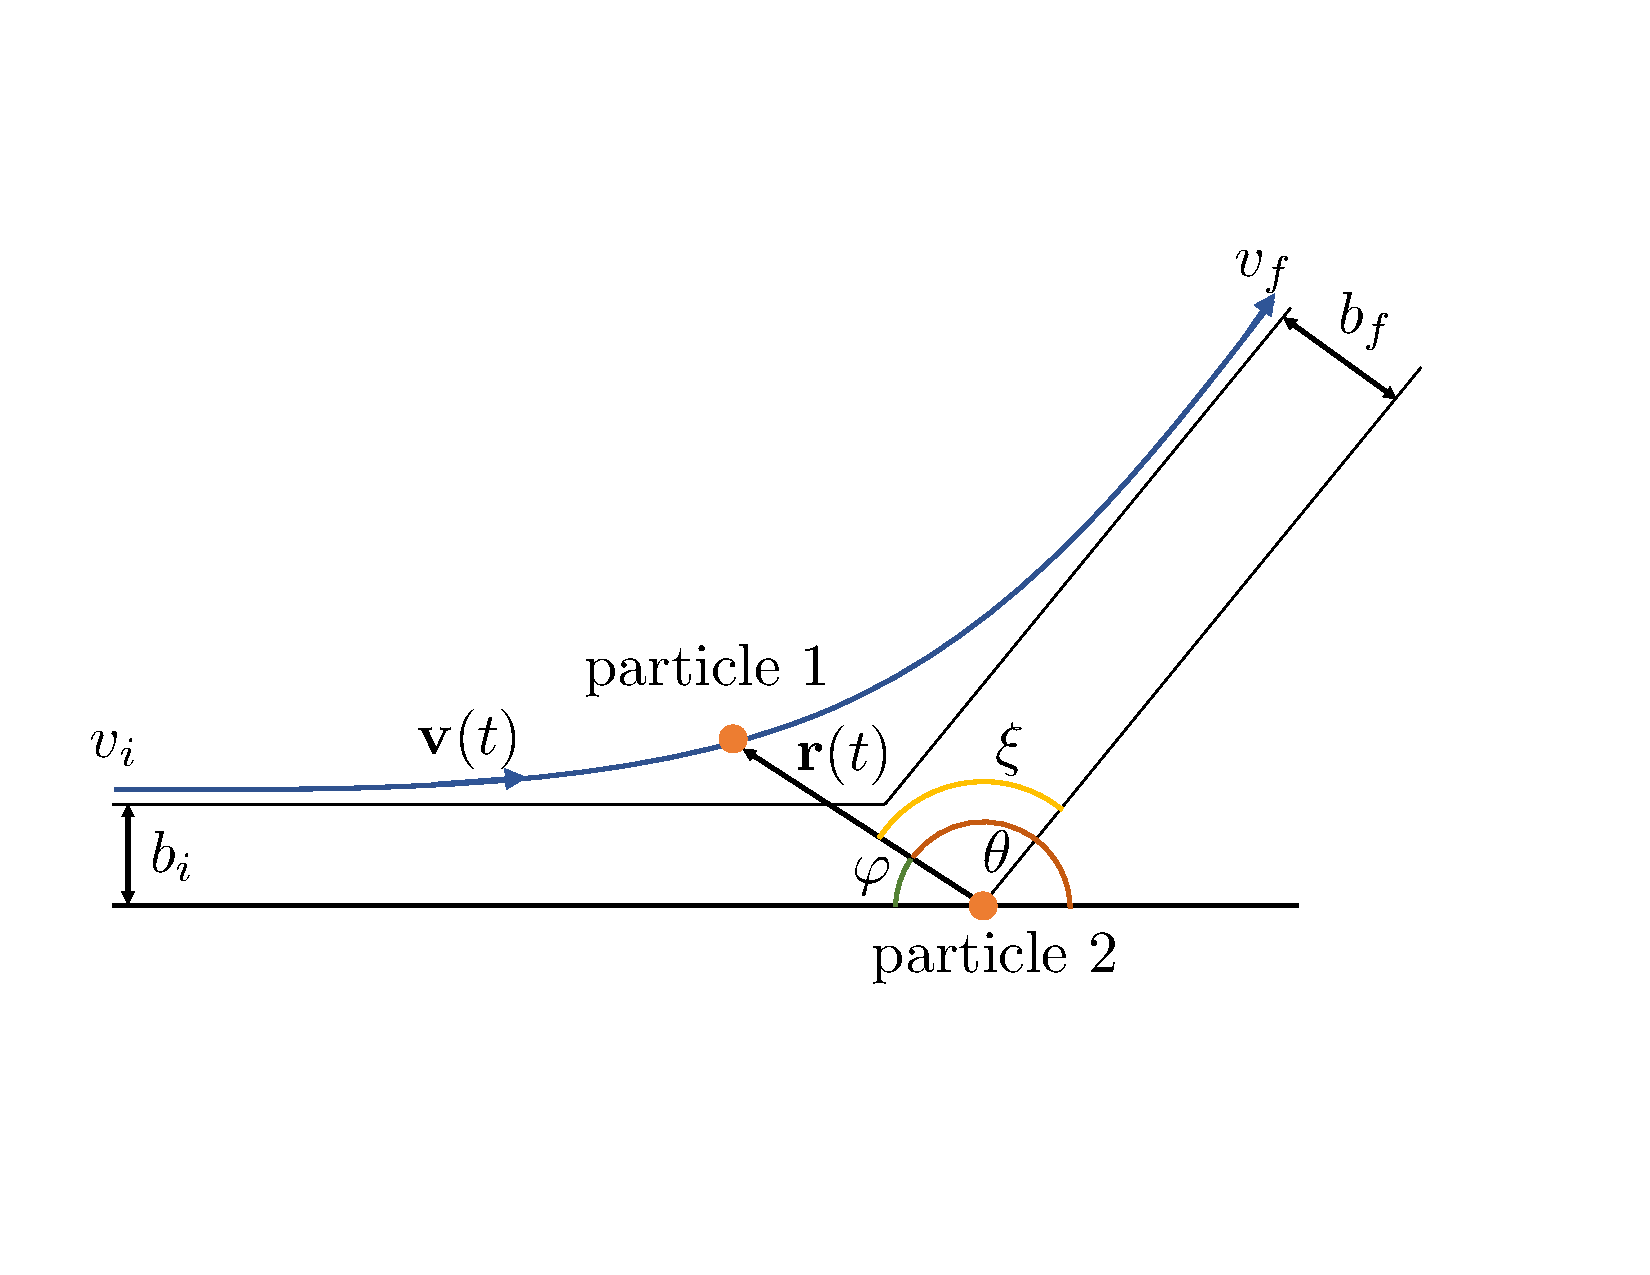
\includegraphics[width=10cm]{../../images/coulomb_scattering.pdf}
    \caption{Depiction of Coulomb scattering.}
    \label{fig:coulomb_scattering}
\end{figure}

If we refer to the plane shown in \cref{fig:coulomb_scattering} as the $x-y$ plane, then one can tell that the angular-momentum vector points in the negative $z$ direction. We will denote the magnitude of the conserved angular momentum by $L$, and thus we can write
\begin{equation}
    \label{eq:coul_cons_angular_momentum}
    m_r \left (\rvec \times \vvec \right ) = -L \hat{\zvec}.
\end{equation}

A consequence of both conservation of energy and momentum is as follows. Consider the two limiting states of particle 1---the initial state $v_i$, $b_i$ and the final state $v_f$, $b_f$. Assuming the potential energy is very low at sufficiently early and late times, conservation of energy gives
\begin{equation}
    \frac{1}{2} m_r v_i^2 = \frac{1}{2} m_r v_f^2,
\end{equation}
that is, $v_i=v_f$ (note that for other scattering processes, e.g.\@ Compton scattering, this is not necessarily the case). For the angular momentum of the initial state we have
\begin{multline}
    \label{eq:coul_cons_angular_momentum_derv1}
    m_r \left ( \rvec_i \times \vvec_i \right ) = m_r \sin(-\theta_i) r_i v_i \hat{\zvec} = - m_r \sin(\theta_i) r_i v_i \hat{\zvec} = - m_r \sin(\pi - \varphi_i) r_i v_i \hat{\zvec} \\
    = - m_r \sin(\varphi_i) r_i v_i \hat{\zvec} = -m_r b_i v_i \hat{\zvec}
\end{multline}
Similarly, for the angular momentum of the final state we have
\begin{equation}
    m_r \left ( \rvec_f \times \vvec_f \right ) = m_r \sin(-\xi_f) r_f v_f  \hat{\zvec} = - m_r \sin(\xi_f) r_f v_f \hat{\zvec} = - m_r b_f v_f \hat{\zvec}.
\end{equation}
Equating the last two relationships gives $m_r b_i v_i = m_r b_f v_f$. Since $v_i = v_f$, we finally have $b_i = b_f = b$. Using \cref{eq:coul_cons_angular_momentum} in \cref{eq:coul_cons_angular_momentum_derv1}, we can also write
\begin{equation}
    \label{eq:coul_cons_angular_momentum_mag}
    L = m_r b v_i.
\end{equation}

%--------------------------------------------
\subsection{Polar coordinates}
%--------------------------------------------
\begin{figure}[ht]
    \centering
    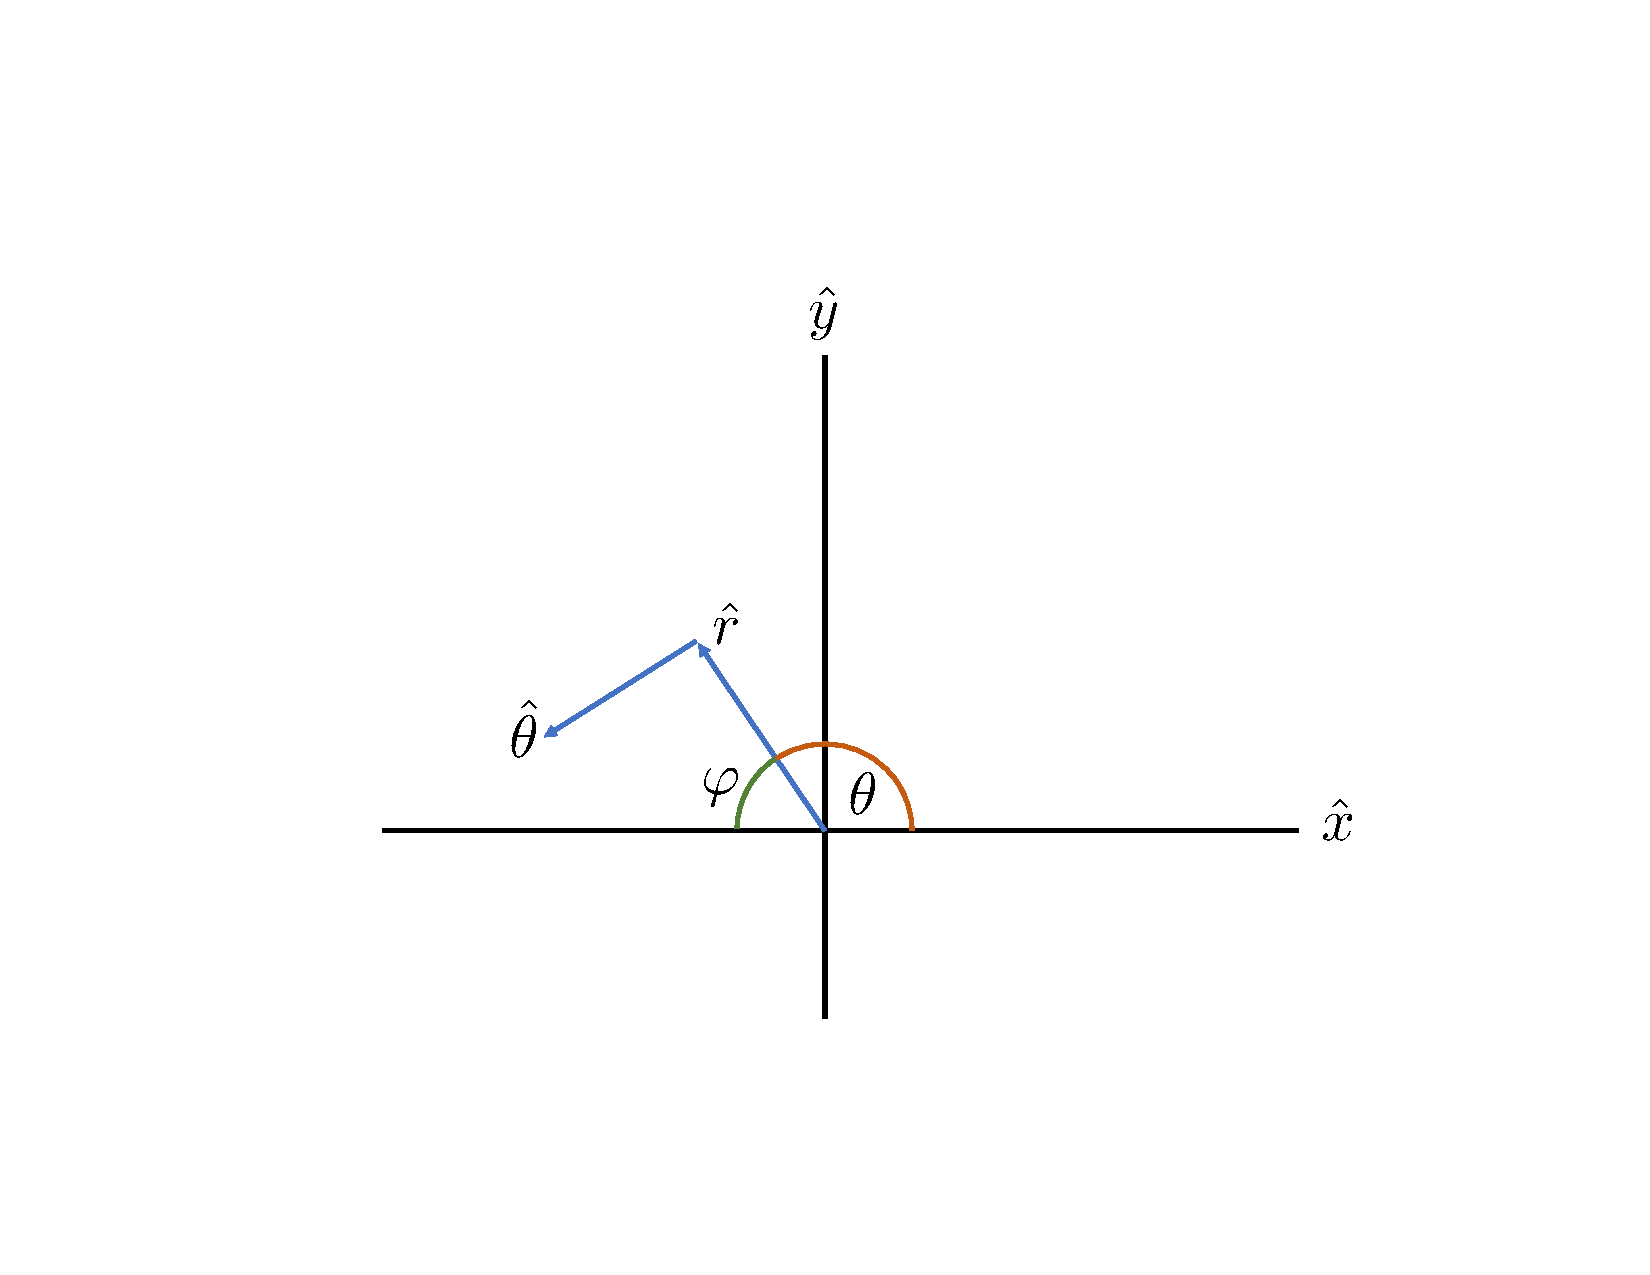
\includegraphics[width=10cm]{../../images/polar_coordinates.pdf}
    \caption{Polar coordinates in plane of interaction.}
    \label{fig:polar_coordinates}
\end{figure}

Using polar coordinates, as shown in \cref{fig:polar_coordinates}, we get
\begin{equation*}
    r_x = r \cos \theta = r \cos ( \pi - \varphi ) = -r \cos \varphi,
\end{equation*}
\begin{equation*}
    r_y = r \sin \theta = r \sin ( \pi - \varphi ) = r \sin \varphi.
\end{equation*}

Also, since $\rvec = r \hat{\rvec}$, we have
\begin{align*}
    \vvec = &\frac{d \rvec}{dt} = \frac{dr}{dt} \hat{\rvec} + r \frac{d\hat{\rvec}}{dt} \nonumber \\
    &= \frac{d r}{dt} \hat{\rvec} + r \frac{d\hat{\rvec}}{d\theta} \frac{d\theta}{dt} \nonumber \\
    &= \frac{dr}{dt} \hat{\rvec} + r \frac{d \theta}{dt} \hat{\bm{\theta}},
\end{align*}
and
\begin{align*}
    \frac{d \vvec}{dt} &= \frac{d^2r}{dt^2} \hat{\rvec} + \frac{dr}{dt} \frac{d\hat{\rvec}}{dt} + \frac{d}{dt} \left ( r \frac{d\theta}{dt} \right ) \hat{\bm{\theta}} + r \frac{d \theta}{dt} \frac{d \hat{\bm{\theta}}}{dt} \nonumber \\
    &= \frac{d^2 r}{dt^2} \hat{\rvec} + \frac{dr}{dt} \frac{d\hat{\rvec}}{d\theta} \frac{d\theta}{dt} + \frac{d}{dt} \left ( r \frac{d\theta}{dt} \right ) \hat{\bm{\theta}} + r \frac{d \theta}{dt} \frac{d \hat{\bm{\theta}}}{d\theta} \frac{d \theta}{dt} \nonumber \\
    &= \frac{d^2r}{dt^2} \hat{\rvec} + \frac{dr}{dt} \frac{d\theta}{dt} \hat{\bm{\theta}} + \frac{d}{dt} \left ( r \frac{d\theta}{dt} \right ) \hat{\bm{\theta}} - r \left ( \frac{d\theta}{dt} \right ) ^2 \hat{\rvec}.
\end{align*}

The radial component of \cref{eq:coul_particle_vel} thus becomes 
\begin{equation*}
    \frac{d^2 r}{dt^2} - r \left ( \frac{d\theta}{dt} \right )^2 = \frac{q_1 q_2}{4 \pi \epsilon_0 m_r} \frac{1}{r^2}.
\end{equation*}
Since $\theta = \pi - \varphi$, we have
\begin{equation}
    \label{eq:coul_particle_position_ode}
    \frac{d^2 r}{dt^2} - r \left ( \frac{d\varphi}{dt} \right )^2 = \frac{q_1 q_2}{4 \pi \epsilon_0 m_r} \frac{1}{r^2}.
\end{equation}

For the angular momentum we have
\begin{equation*}
    m_r \rvec \times \vvec = m_r r \hat{\rvec} \times \left ( \frac{dr}{dt} \hat{\rvec} + r \frac{d\theta}{dt} \hat{\bm{\theta}} \right ) = m_r r^2 \frac{d\theta}{dt} \hat{\zvec}
\end{equation*}
Using \cref{eq:coul_cons_angular_momentum}, we can write the above as
\begin{equation}
    \label{eq:coul_particle_cons_angular_polar}
    m_r r^2 \frac{d\varphi}{dt} = L.
\end{equation}

%--------------------------------------------
\subsection{Particle trajectory}
%--------------------------------------------
The goal is to find the radial position of the particle as a function of its angular orientation. That is, we want to find $\tilde{r} = \tilde{r}(\tilde{\varphi})$ such that
\begin{equation}
    \label{eq:coul_particle_position_angle}
    r(t) = \tilde{r}(\varphi(t)).
\end{equation}
To simplify the math, we introduce $\tilde{u} = \tilde{u}(\tilde{\varphi})$ such that $\tilde{u} = 1 / \tilde{r}$. Thus
\begin{equation*}
    \frac{d \tilde{u}}{d\tilde{\varphi}} = -\frac{1}{\tilde{r}^2} \frac{d \tilde{r}}{d\tilde{\varphi}},
\end{equation*}
or, after re-arranging
\begin{equation}
    \label{eq:coul_rgrad_vs_ugrad}
    \frac{d \tilde{r}}{d\tilde{\varphi}} = -\frac{1}{\tilde{u}^2} \frac{d \tilde{u}}{d\tilde{\varphi}}.
\end{equation}

We now proceed as follows. Taking the derivative of $r$, we get
\begin{align}
    \label{eq:coul_particle_derivation_1}
    \frac{dr}{dt} &= \left ( \frac{d \tilde{r}}{d\tilde{\varphi}} \right )_{\tilde{\varphi} = \varphi(t)} \frac{d \varphi}{dt} &&[\cref{eq:coul_particle_position_angle}] \nonumber \\
    &= \left ( -\frac{1}{\tilde{u}^2} \frac{d\tilde{u}}{d\tilde{\varphi}} \right )_{\tilde{\varphi} = \varphi(t)} \frac{d \varphi}{dt} &&[\cref{eq:coul_rgrad_vs_ugrad}]\nonumber \\ 
    &= \left ( -\frac{1}{\tilde{u}^2} \frac{d\tilde{u}}{d\tilde{\varphi}} \right )_{\tilde{\varphi} = \varphi(t)} \frac{L}{m_r r^2} &&[\cref{eq:coul_particle_cons_angular_polar}] \nonumber \\
    &= \left ( -\frac{1}{\tilde{u}^2} \frac{d\tilde{u}}{d\tilde{\varphi}} \frac{L}{m_r \tilde{r}^2} \right )_{\tilde{\varphi} = \varphi(t)} &&[\cref{eq:coul_particle_position_angle}] \nonumber \\
    &= \left ( - \frac{d\tilde{u}}{d\tilde{\varphi}} \frac{L}{m_r} \right )_{\tilde{\varphi} = \varphi(t)}
\end{align}
Taking the derivative of the above, we get
\begin{align}
    \frac{d}{dt} \frac{dr}{dt} &= \left [ \frac{d}{d\tilde{\varphi}} \left ( - \frac{d\tilde{u}}{d\tilde{\varphi}} \frac{L}{m_r} \right ) \right ]_{\tilde{\varphi} = \varphi(t)} \frac{d \varphi}{dt} \nonumber \\
    &= \left ( - \frac{d^2 \tilde{u}}{d\tilde{\varphi}^2} \frac{L}{m_r} \right )_{\tilde{\varphi} = \varphi(t)} \frac{L}{m_r r^2} && [\cref{eq:coul_particle_cons_angular_polar}] \nonumber \\
    &= \left ( - \frac{d^2 \tilde{u}}{d\tilde{\varphi}^2} \frac{L}{m_r} \frac{L}{m_r \tilde{r}^2} \right )_{\tilde{\varphi} = \varphi(t)} && [\cref{eq:coul_particle_position_angle}] \nonumber \\
    &= \left ( - \frac{d^2 \tilde{u}}{d\tilde{\varphi}^2} \frac{L^2 \tilde{u}^2}{m_r^2} \right )_{\tilde{\varphi} = \varphi(t)}
\end{align}
Plugging the last relation into \cref{eq:coul_particle_position_ode} gives
\begin{equation*}
    \left [ - \frac{d^2 \tilde{u}}{d\tilde{\varphi}^2} \frac{L^2 \tilde{u}^2}{m_r^2} - \frac{1}{\tilde{u}} \left ( \frac{L \tilde{u}^2}{m_r} \right )^2 \right ]_{\tilde{\varphi} = \varphi(t)} = \left ( \frac{q_1 q_2}{4 \pi \epsilon_0 m_r} \tilde{u}^2 \right )_{\tilde{\varphi} = \varphi(t)},
\end{equation*}
which, upon re-arranging and dropping the $\varphi(t)$ dependance, becomes
\begin{equation}
    \frac{d^2 \tilde{u}}{d \tilde{\varphi}^2} + \tilde{u} = -\frac{q_1 q_2 m_r}{4 \pi \epsilon_0 L^2}
\end{equation}

Using \cref{eq:coul_cons_angular_momentum_mag} we write the evolution equation for $\tilde{u}$ as
\begin{equation}
    \frac{d^2 \tilde{u}}{d \tilde{\varphi}^2} + \tilde{u} = -\frac{q_1 q_2}{4 \pi \epsilon_0 m_r b^2 v_i^2}.
\end{equation}
Introducing the notation
\begin{equation}
    \label{eq:coul_b90}
    b_{90} = \frac{q_1 q_2}{4 \pi \epsilon_0 m_r v_i^2},
\end{equation}
the evolution equation for $\tilde{u}$ can be simply expressed as
\begin{equation}
    \label{eq:coul_particle_u_equation}
    \frac{d^2 \tilde{u}}{d \tilde{\varphi}^2} + \tilde{u} = -\frac{b_{90}}{b^2}.
\end{equation}

The boundary conditions for \cref{eq:coul_particle_u_equation} are as follows
\begin{equation}
    \label{eq:coul_particle_bc_1}
    \text{as } \varphi(t) \to 0, \quad r(t) \to \infty
\end{equation}
\begin{equation}
    \label{eq:coul_particle_bc_2}
    \text{as } \varphi(t) \to 0, \quad \frac{dr(t)}{dt} \to -v_i
\end{equation}
Given \cref{eq:coul_particle_position_angle}, \cref{eq:coul_particle_bc_1} can only be satisfied if as $\tilde{\varphi} \to 0$, $\tilde{r} \to \infty$. Thus, we also have, as $\tilde{\varphi} \to 0$, $\tilde{u} \to 0$. Similarly, given \cref{eq:coul_particle_derivation_1}, \cref{eq:coul_particle_bc_2} can only be satisfied if as $\tilde{\varphi} \to 0$
\begin{equation*}
    \frac{d\tilde{u}}{d\tilde{\varphi}} \frac{L}{m_r} \to v_i.
\end{equation*}
Using \cref{eq:coul_cons_angular_momentum_mag} we rewrite the above as 
\begin{equation*}
    \frac{d\tilde{u}}{d\tilde{\varphi}} \to \frac{1}{b}.
\end{equation*}

The general solution to \cref{eq:coul_particle_u_equation} is 
\begin{equation*}
    \tilde{u} = A \cos \tilde{\varphi} + B \sin \tilde{\varphi} - \frac{b_{90}}{b^2}.
\end{equation*}
Applying the boundary conditions, we get
\begin{equation*}
    \tilde{u} = \frac{b_{90}}{b^2} \cos \tilde{\varphi} + \frac{1}{b} \sin \tilde{\varphi} - \frac{b_{90}}{b^2},
\end{equation*}
which we finally re-write as
\begin{equation}
    \label{eq:coul_trajectory_eq}
    \frac{1}{\tilde{r}} = \frac{1}{b} \sin \tilde{\varphi} + \frac{b_{90}}{b^2} \left ( \cos \tilde{\varphi} - 1 \right ).
\end{equation}

%--------------------------------------------
\subsection{The scattering angle}
%--------------------------------------------
We now drop the tilde notation for the sake of simplicity. That is, for the radial location of an incident particle, we have
\begin{equation}
    \label{eq:coul_trajectory_eq2}
    \frac{1}{r} = \frac{1}{b} \sin \varphi + \frac{b_{90}}{b^2} \left ( \cos \varphi - 1 \right ),
\end{equation}
where $\varphi$ is the independent variable and $r = r(\varphi)$. We want to know the value of $\varphi$ as $r$ goes to infinity. Using \cref{eq:coul_trajectory_eq2}, and labeling this angle as $\varphi_s$, we have
\begin{equation*}
    0 = \sin \varphi_s + \frac{b_{90}}{b} \left ( \cos \varphi_s - 1 \right ).
\end{equation*}
We express the above in terms of the scattering angle $\theta_s = \pi - \varphi_s$,
\begin{equation*}
    0 = \sin (\pi - \theta_s) + \frac{b_{90}}{b} \left [ \cos \left (\pi - \theta_s \right ) - 1 \right ].
\end{equation*}
or
\begin{equation*}
    0 = \sin \theta_s + \frac{b_{90}}{b} \left ( -\cos \theta_s - 1 \right ).
\end{equation*}
Re-writing the above as
\begin{equation*}
    \frac{\cos \theta_s + 1}{\sin \theta_s} = \frac{b}{b_{90}},
\end{equation*}
and using the trig identity $\cot (\theta/2) = (\cos \theta + 1) / \sin \theta$, we get 
\begin{equation}
    \label{eq:coul_scattering_angle}
    \cot \left ( \frac{ \theta_s }{2} \right ) = \frac{b}{b_{90}}.
\end{equation}

%--------------------------------------------
\subsection{The differential cross section}
%--------------------------------------------

The differential cross section for Coulomb scattering can be computed by making use of \cref{eq:cross_diff_impact_axi}, which is repeated below
\begin{equation}
    \tag{\ref{eq:cross_diff_impact_axi}}
    \frac{d\sigma_\theta}{d\Omega} = \frac{b}{\sin \theta_s} \left | \frac{db}{d\theta_s} \right |.
\end{equation}
From \cref{eq:coul_scattering_angle} we get,
\begin{equation}
    \frac{db}{d\theta} = -\frac{b_{90}}{2} \frac{1}{\sin^2 (\theta_s / 2)},
\end{equation}
which, plugging in \cref{eq:cross_diff_impact_axi}, gives
\begin{equation*}
    \frac{d\sigma_\theta}{d\Omega} = \left [ b_{90}\frac{\cot(\theta_s/2)}{\sin \theta_s} \right ] \left [ \frac{b_{90}}{2} \frac{1}{\sin^2 (\theta_s / 2)} \right ].
\end{equation*}
Using the trig identities $\cot(\theta) = \cos(\theta) / \sin(\theta)$ and $\sin(\theta) = 2 \sin(\theta/2) \cos(\theta/2)$ we get
\begin{equation}
    \frac{d\sigma_\theta}{d\Omega} = \frac{b_{90}^2}{4} \frac{1}{\sin^4 (\theta_s/2)}.
\end{equation}

%--------------------------------------------
\subsection{Collision integral}
%--------------------------------------------
\begin{equation}
    \Omega_{\alpha \beta}^{(lk)} = \sqrt{ \frac{k_B T}{2 \pi M_{\alpha \beta}} } \int_0^\infty e^{-g^2} g^{2k+3} \phi_{\alpha \beta}^{(l)} \, dg.
\end{equation}
In the above $M_{\alpha \beta}$ is the reduced mass, given by
\begin{equation}
    M_{\alpha \beta} = \frac{M_\alpha M_\beta}{M_\alpha + M_\beta},
\end{equation}
and $\phi^{(l)}_{\alpha \beta}$ is the collision cross section for a given velocity, and is computed as
\begin{equation}
    \phi_{\alpha \beta}^{(l)} = 2 \pi \int_0^\infty \left ( 1 - \cos^l \chi_{\alpha \beta} \right ) b \, db.
\end{equation}
The scattering angle $\chi_{\alpha \beta}$ is given by
\begin{equation}
    \chi_{\alpha \beta} = \pi - 2 \int_{r_{\alpha \beta}^{\text{min}}}^\infty \frac{b}{r^2 \left [ 1 - \frac{b^2}{r^2} - \frac{V_{\alpha \beta (r)}}{g^2 k_B T} \right ]^{1/2} } \, dr.
\end{equation}

For a Coulombic interaction between ions, we can define the natural scale fore the cross-sectional area as
\begin{equation}
    \phi^{(0)}_{\alpha \beta} = \frac{ \pi \left (Z_\alpha Z_\beta e^2 \right)^2}{ \left(2 k_B T\right)^2}.
\end{equation}
Given this definition, we express the collision integral as
\begin{equation}
    \Omega_{\alpha \beta} = \sqrt{ \frac{\pi }{M_{\alpha \beta}}} \frac{( Z_\alpha Z_\beta e^2)^2 }{(2 k_B T )^{3/2}} \mathcal{F}^{lk}_{\alpha \beta},
\end{equation}
where
\begin{equation}
    \mathcal{F}^{(lk)}_{\alpha \beta} = \frac{1}{2 \phi_0} \int_0^\infty e^{-g^2} g^{2k+3} \phi_{\alpha \beta}^{(l)} \, dg
\end{equation}
We note that $\mathcal{F}^{(lk)}_{\alpha \beta} = 4 \mathcal{K}_{lk}(g_{\alpha \beta})$, where $\mathcal{K}_{lk}(g_{\alpha \beta})$ is the notation from the Stanton-Murillo paper.

\end{document}
